\documentclass[11pt]{article}

\usepackage[paperwidth=8.5in, paperheight=13in, top=0.75in, bottom=0.75in, right=0.75in, left=1.25in]{geometry}

\usepackage[utf8]{inputenc}
\usepackage{amsmath, amssymb, amsfonts, mathtools, bm, mathrsfs, esvect, harpoon}

\usepackage{graphicx, xcolor, tikz, pgfplots}
\usepackage[siunitx, american]{circuitikz} % For Electrical Network problems

\usetikzlibrary{
    arrows.meta, 
    positioning, 
    decorations.pathmorphing, 
    decorations.markings, 
    patterns, 
    calc, 
    shapes.geometric
}

\pgfplotsset{compat=1.18}

\usepackage{fancybox, verbatim, xspace, setspace, multicol, ifthen, calc, fancyhdr, enumitem, textcomp, array}


% Styles
\tikzset{
    % BLOCK DIAGRAM ALGEBRA
    spring/.style={
        decoration={
          coil,
          aspect=0.6,
          segment length=2.3mm,
          amplitude=2.3mm,
          pre length=3mm,
          post length=3mm
        },
        decorate
    },
    block/.style={
        rectangle,
        draw,
        minimum height=10mm,
        minimum width=10mm,
        align=center
    },
    sumpoint/.style={
        circle, 
        draw, 
        minimum size=7mm, 
        thick,
        path picture={
            \draw[black, thick]
            (path picture bounding box.south west) -- (path picture bounding box.north east)
            (path picture bounding box.north west) -- (path picture bounding box.south east);
        }
    },
    tpoint/.style={
        circle,         
        fill=black,    
        inner sep=0pt, 
        minimum size=1.5mm 
    },
    wall/.style={
        pattern=north west lines,
        draw,
        minimum width=2mm,
        minimum height=30mm
    },
    tbody/.style={
        rectangle,
        draw,
        minimum height=27mm, 
        minimum width=20mm, 
        align=center
    },
    mid arrow/.style={
        postaction={
          decorate,
          decoration={
            markings,
            mark=at position 0.5 with {\arrow[scale=1.5]{>}}
          }
        }
    }
}

% Macros
    %summing point
    \newcommand{\summingpointwithsignsat}[6][]{%
        \node[sumpoint, #1] (#6) {};
        \node at ([yshift=2mm]#6.center) {$#2$};   % top
        \node at ([xshift=-2mm]#6.center)  {$#3$};  % left
        \node at ([yshift=-2mm]#6.center) {$#4$};  % bottom
        \node at ([xshift=2mm]#6.center)  {$#5$};   % right
    }

    % spring
    \newcommand{\hspring}[2]{%
      \draw[spring] (#1) -- ++(2,0) node[midway, above=0.25cm]{#2};
    }
    \newcommand{\blspring}[2]{%
      \draw[spring] (#1) -- ++(2,0) node[midway, below=0.25cm]{#2};
    }

    %damper
    \newcommand{\hdamper}[2]{%
      \begin{scope}[shift={#1}]
        % Damper body (shifted right by 0.5)
        \draw (0,0) -- (0.5,0);                  % Left line
        \draw (0.5,0) -- (0.5,0.3) -- (1.5,0.3);  % Top bar
        \draw (0.5,0) -- (0.5,-0.3) -- (1.5,-0.3);% Bottom bar
        
        % Dash lines / piston
        \draw (1.0,0) -- (1.0,0.15);
        \draw (1.0,0) -- (1.0,-0.15);
        
        % Output line
        \draw (1.0,0) -- (2.0,0);
    
        % Label above the damper
        \node[above] at (1,0.3) {#2};
      \end{scope}
    }
    \newcommand{\bldamper}[2]{%
      \begin{scope}[shift={#1}]
        % Damper body (shifted right by 0.5)
        \draw (0,0) -- (0.5,0);                  % Left line
        \draw (0.5,0) -- (0.5,0.3) -- (1.5,0.3);  % Top bar
        \draw (0.5,0) -- (0.5,-0.3) -- (1.5,-0.3);% Bottom bar
        
        % Dash lines / piston
        \draw (1.0,0) -- (1.0,0.15);
        \draw (1.0,0) -- (1.0,-0.15);
        
        % Output line
        \draw (1.0,0) -- (2.0,0);
    
        % Label below the damper
        \node[below] at (1,-0.3) {#2};
      \end{scope}
    }

    % mass
    \newcommand{\tbody}[4]{
    \node[tbody] (#4) at (#1) {#2};
    \node at ([yshift=20mm]#4.center) {#3};
    \draw ([yshift=11mm]#4.center) -- ([yshift=18mm]#4.center);
    \draw[->] ([yshift=16mm, xshift=-4mm]#4.center) -- ([yshift=16mm, xshift=5mm]#4.center);
    }
    \newcommand{\rbody}[3]{%
      \begin{scope}[shift={#1}]
        \draw (0,0) -- (1,0);
        \draw (1,0) ellipse (0.2 and 0.5);
    
        % Top and bottom walls
        \draw (1,0.5) -- (3.3,0.5);
        \draw (1,-0.5) -- (3.3,-0.5);
        \draw (3.5,0) ++(0,0) arc[start angle=0, end angle=90, x radius=0.2, y radius=0.5];
        \draw (3.5,0) ++(0,0) arc[start angle=0, end angle=-90, x radius=0.2, y radius=0.5];
        \draw (3.5,0) -- (4,0);
        \node at (2.2,0) {#2};
        % Theta
        \draw[->] (0.5,-0.7) arc[start angle=-90, end angle=-325, x radius=0.2, y radius=0.8];
        \node at (0.5,1.2) {#3};
      \end{scope}
    }
    \newcommand{\frbody}[1]{%
      \begin{scope}[shift={#1}]
        \draw (0,0) -- (1,0);
        \draw (1,0) ellipse (0.2 and 0.5);
    
        % Top and bottom walls
        \draw (1,0.5) -- (3.3,0.5);
        \draw (1,-0.5) -- (3.3,-0.5);
    
        \draw (3.5,0) ++(0,0) arc[start angle=0, end angle=90, x radius=0.2, y radius=0.5];
        \draw (3.5,0) ++(0,0) arc[start angle=0, end angle=-90, x radius=0.2, y radius=0.5];
    
        \draw (3.5,0) -- (4,0);
    
        \node at (2.2,0) {$J_1$};
    
        % Theta
        \draw[->] (0.4,-0.7) arc[start angle=-90, end angle=-325, x radius=0.2, y radius=0.8];
        \draw[->] (0.9,-0.7) arc[start angle=-90, end angle=-325, x radius=0.2, y radius=0.8];
    
        \node at (0.4,1.2) {$T(t)$};
        \node at (1.2,1.2) {$\theta_1(t)$};
      \end{scope}
    }
    \newcommand{\ccrbody}[3]{%
      \begin{scope}[shift={#1}]
       \draw (0,0) -- (1,0);
        \draw (1,0) ellipse (0.2 and 0.5);
        % Top and bottom walls
        \draw (1,0.5) -- (3.3,0.5);
        \draw (1,-0.5) -- (3.3,-0.5);
        \draw (3.5,0) ++(0,0) arc[start angle=0, end angle=90, x radius=0.2, y radius=0.5];
        \draw (3.5,0) ++(0,0) arc[start angle=0, end angle=-90, x radius=0.2, y radius=0.5];
        \draw (3.5,0) -- (4,0);
        \node at (2.2,0) {#2};
        % Theta
        \draw[->] (0.45,-0.7) arc[start angle=-100, end angle=145, x radius=0.2, y radius=0.8];
        \node at (0.5,1.2) {#3};
      \end{scope}
    }
    
    %gear
    \newcommand{\gearpair}[3]{
        \begin{scope}[shift={#1}]
            \draw (0,0.8) -- (0,-0.8);     
            \draw (0,-1.2) -- (0,-2.8); 
            \node at (0,1.1) {#2};         % top label
            \node at (0,-3.1) {#3};        % bottom label
        \end{scope}
    }
    
    %wall
    \newcommand{\rwall}[1]{%
      \node[wall] at ($(#1)+(0.12,0)$) {};
    }
    
    %dcmotor
    \newcommand{\dcmotor}[0]{%
        \draw (-1.5,-0.75) rectangle (0,0.75);
        \node at (-0.75,0) {Motor};
        
        \draw (-2.3,0.5) -- (-1.5,0.5);
        \node at (-2,0.3) {$+$};
        \node at (-2,0) {$e_a$};
        \node at (-2,-0.3) {$-$};
        \draw (-2.3,-0.5) -- (-1.5,-0.5);
    }
    
    %signal flow
    \newcommand{\uloop}[3]{%
      \draw[mid arrow] #2 to[bend right=60] #1;
      \node at ($#1 + (1.5,0.3)$) {#3};
    }
    
    \newcommand{\forw}[2]{%
        \draw[mid arrow] #1 -- #2;
        \fill #1 circle (3pt);
        \fill #2 circle (3pt);
    }

\begin{document}
  \thispagestyle{empty} 

  \begin{figure}
    \centering
    %change the file name of your pup logo similarly to {pup-logo.png} 
    
\includegraphics[width=0.2\textwidth]{pup-logo.png}
  \end{figure}

  \begin{center}
    {\Large
    Polytechnic University of the Philippines\\
    College of Engineering\\
    Computer Engineering Department\\
    }
  \end{center}

\vfill

  \begin{center}
    {\Large \textbf{Solved Problems in Feedback and Control Systems}} \\ 
    {\large (Electrical Network Transfer Functions,
Translational Mechanical System Transfer \\Functions,
Rotational Mechanical System Transfer Functions,
Transfer Function \\involving Gears, 
Electromechanical System Transfer Function,
Block Diagram \\Algebra, and Signal Flow Graphs)}
  \end{center}

\vfill

  \begin{center}
    {\large
    Completion requirement for the subject\\
    CMPE 309 - Feedback and Control Systems\\
    }
  \end{center}

\vfill

  \begin{center}
    {\large 
    YAMBOT, Cedric G. \\ % name
    2023-18849-MN-1\\ % student number
    Bachelor of Science in Computer Engineering\\
    }
  \end{center}

\vfill

  \begin{center}
    Engr. John R. Dela Cruz, MSECE, PECE, AAE, 1PHN\\
    Faculty-in-charge
  \end{center}

\vfill

  \begin{center}
    % month kung kailan mo ipapasa 'yung completion, remove square brackets 
    % ex: August 2025
    May 2026
  \end{center}

% Problem 1 - Electrical Network 
\newpage
  \setcounter{page}{1}  
\noindent\rule{\textwidth}{1pt}
\noindent\textbf{Problem 1} \hfill

\noindent Given the electrical network diagram below, determine the transfer function $G(s) = I_3(s)/V_i(s)$.

% problem 1 - figure

\begin{figure}[!htbp]
    \centering
    \resizebox{\textwidth}{!}{%
    \begin{circuitikz}

    \draw (0,0) to [V, invert, l=$v_i(t)$] (0,6)
        to [L, l=$L_1$] (2,6)
        to [R, l=$R_1$] (4,6)
        to [cC, l=$C_1$] (6,6)
        to [L, l=$L_4$] (8,6)
        to [R, l=$R_4$] (10,6)
        to [cC, l=$C_4$] (12,6)
        to [L, l=$L_7$] (14,6)
        to [R, l=$R_7$] (16,6)
        to [cC, l=$C_7$] (18,6)
        to [L, l=$L_9$] (18,4)
        to [R, l=$R_9$] (18,2)
        to [cC, l=$C_9$] (18,0)
        to [cC, l=$C_8$] (16,0)
        to [R, l=$R_8$] (14,0)
        to [L, l=$L_8$] (12,0)
        to [cC, l=$C_5$] (10,0)
        to [R, l=$R_5$] (8,0)
        to [L, l=$L_5$] (6,0)
        to [cC, l=$C_2$] (4,0)
        to [R, l=$R_2$] (2,0)
        to [L, l=$L_2$] (0,0);

    \draw (6,6) to [L, l=$L_3$] (6,4)
        to [R, l=$R_3$] (6,2)
        to [cC, l=$C_3$] (6,0);

    \draw (12,6) to [L, l=$L_6$] (12,4)
        to [R, l=$R_6$] (12,2)
        to [cC, l=$C_6$] (12,0);
     
    \draw[->, thick] (3,3) ++(-1,0) arc[start angle=180, end angle=-120, radius=1];
    \node at (3,3) {$i_1(t)$};

    \draw[->, thick] (9,3) ++(-1,0) arc[start angle=180, end angle=-120, radius=1];
    \node at (9,3) {$i_2(t)$};

    \draw[->, thick] (15,3) ++(-1,0) arc[start angle=180, end angle=-120, radius=1];
    \node at (15,3) {$i_3(t)$};
     
    \end{circuitikz}
    }
    
\end{figure}

% problem statement

\noindent\rule{\textwidth}{1pt}

\vspace{12pt}

\noindent\textbf{\textit{Given:}}
\[
\begin{aligned}
R_1 &= 1\, \Omega & L_1 &= 1\, \text{H} & C_1 &= 1\, \text{F} \\
R_2 &= 1\, \Omega & L_2 &= 1\, \text{H} & C_2 &= 1\, \text{F} \\
R_3 &= 1\, \Omega & L_3 &= 1\, \text{H} & C_3 &= 1\, \text{F} \\
R_4 &= 1\, \Omega & L_4 &= 1\, \text{H} & C_4 &= 1\, \text{F} \\
R_5 &= 1\, \Omega & L_5 &= 1\, \text{H} & C_5 &= 1\, \text{F} \\
R_6 &= 1\, \Omega & L_6 &= 1\, \text{H} & C_6 &= 1\, \text{F} \\
R_7 &= 1\, \Omega & L_7 &= 1\, \text{H} & C_7 &= 1\, \text{F} \\
R_8 &= 1\, \Omega & L_8 &= 1\, \text{H} & C_8 &= 1\, \text{F} \\
R_9 &= 1\, \Omega & L_9 &= 1\, \text{H} & C_9 &= 1\, \text{F}
\end{aligned}
\]

\vspace{12pt}

\noindent \textbf{\textit{Required:}}
\[
G(s) = \frac{I_3(s)}{V_i(s)}
\]

\vspace{12pt}

\noindent \textbf{\textit{Solution:}}

\bigskip

{System of Equations:}
\[
\begin{aligned}
(3K)I_1(s) - (K)I_2(s) &= V_i(s) \\
-(K)I_1(s) + (4K)I_2(s) - (K)I_3(s) &= 0 \\
-(K)I_2(s) + (4K)I_3(s) &= 0
\end{aligned}
\]

{where $K = \frac{s^2 + s + 1}{s}$.}

{Matrix Form:}
\[
\begin{bmatrix}
3K & -K & 0 \\
-K & 4K & -K \\
0 & -K & 4K
\end{bmatrix}
\begin{bmatrix}
I_1(s) \\ I_2(s) \\ I_3(s)
\end{bmatrix}
=
\begin{bmatrix}
V_i(s) \\ 0 \\ 0
\end{bmatrix}
\]

{Determinant \(\Delta\):}
\[
\Delta =
\begin{vmatrix}
3K & -K & 0 \\
-K & 4K & -K \\
0 & -K & 4K
\end{vmatrix}
= 41K^3
\]

{Using Cramer's Rule for \(I_3(s)\):}
\[
I_3(s) =
\frac{
\begin{vmatrix}
3K & -K & V_i(s) \\
-K & 4K & 0 \\
0 & -K & 0
\end{vmatrix}
}
{\Delta}
= \frac{K^2 V_i(s)}{41K^3} = \frac{V_i(s)}{41K}
\]\newline

{Transfer Function:}

\[
\boxed{
G(s) = \frac{I_3(s)}{V_i(s)} = \frac{s}{41s^2 + 41s + 41}
}
\]


% Problem 2 - electrical networks

\newpage
  \setcounter{page}{3}  
\noindent\rule{\textwidth}{1pt}
\noindent\textbf{Problem 2} \hfill 

\noindent Given the electrical network diagram below, determine the transfer function $G(s) = I_3(s)/V_i(s)$.

\begin{figure}[!htbp]
    \centering
    \resizebox{0.6\textwidth}{!}{ 
        \begin{circuitikz}

    \draw (0,0) to [V, invert, l=$v_i(t)$] (0,3)
        to [L, l=$L_1$] (0,6)
        to [L, l=$L_2$] (6,6)
        to [L, l=$L_3$] (6,3)
        to [R, l=$R_3$] (6,0)
        to [R, l=$R_2$] (3,0)
        to [cC, l=$C_2$] (0,0);

    \draw (0,3) to [cC, l=$C_1$] (3,3)
        to [R, l=$R_1$] (6,3);

    \draw (3,3) [cC, l=$C_3$] to (3,0);

    \draw[->, thick] (3, 4.5) ++(-0.8,0) arc[start angle=180, end angle=-120, radius=0.8];
    \node at (3,4.5) {$i_1(t)$};
     
    \draw[->, thick] (1.5,1.5) ++(-0.8,0) arc[start angle=180, end angle=-120, radius=0.8];
    \node at (1.5,1.5) {$i_2(t)$};

    \draw[->, thick] (4.5,1.5) ++(-0.4,0) arc[start angle=180, end angle=-120, radius=0.8];
    \node at (4.9,1.5) {$i_3(t)$};
     
    \end{circuitikz}
    }
\end{figure}

\noindent\rule{\textwidth}{1pt}

\vspace{12pt}

\noindent\textbf{\textit{Given:}}
\[
\begin{aligned}
R_1 &= 1\, \Omega & L_1 &= 1\, \text{H} & C_1 &= 1\, \text{F} \\
R_2 &= 1\, \Omega & L_2 &= 1\, \text{H} & C_2 &= 1\, \text{F} \\
R_3 &= 1\, \Omega & L_3 &= 1\, \text{H} & C_3 &= 1\, \text{F}
\end{aligned}
\]

\vspace{12pt}

\noindent \textbf{\textit{Required:}}
\[
G(s) = \frac{I_3(s)}{V_i(s)}
\]

\vspace{12pt}

\noindent \textbf{\textit{Solution:}}

\bigskip

{System of Equations:}
\[
\begin{aligned}
(3s^2 + s + 1)I_1(s) - I_2(s) - s I_3(s) &= 0 \\
-I_1(s) + 3I_2(s) - I_3(s) &= sV_i(s) \\
-s I_1(s) - I_2(s) + (2s + 1)I_3(s) &= 0
\end{aligned}
\]

{Matrix Form:}
\[
\begin{bmatrix}
3s^2 + s + 1 & -1 & -s \\
-1 & 3 & -1 \\
-s & -1 & 2s + 1
\end{bmatrix}
\begin{bmatrix}
I_1(s) \\ I_2(s) \\ I_3(s)
\end{bmatrix}
=
\begin{bmatrix}
0 \\ sV_i(s) \\ 0
\end{bmatrix}
\]

{Determinant \(\Delta\):}
\[
\Delta =
\begin{vmatrix}
3s^2 + s + 1 & -1 & -s \\
-1 & 3 & -1 \\
-s & -1 & 2s + 1
\end{vmatrix}
= 18s^3 + 9s^2 + 6s + 1
\]

{Using Cramer's Rule for \(I_3(s)\):}
\[
I_3(s) =
\frac{
\begin{vmatrix}
3s^2 + s + 1 & -1 & 0 \\
-1 & 3 & sV_i(s) \\
-s & -1 & 0
\end{vmatrix}
}
{\Delta}
= \frac{sV_i(s)(3s^2 + 2s + 1)}{18s^3 + 9s^2 + 6s + 1}
\]


{Transfer Function:}

\[
\boxed{
G(s) = \frac{I_3(s)}{V_i(s)} = \frac{3s^3 + 2s^2 + s}{18s^3 + 9s^2 + 6s + 1}
}
\]


% Problem 3

\newpage
  \setcounter{page}{5}
\noindent\rule{\textwidth}{1pt}
\noindent\textbf{Problem 3} \hfill 

\noindent Given the electrical network diagram below, determine the transfer function $G(s) = I_3(s)/V_i(s)$.

\begin{figure}[!htbp]
    \centering
    \resizebox{0.7\textwidth}{!}{
        \begin{circuitikz}
        \draw (0,0) to [V, invert, l=$v_i(t)$] (0,5)
            to [cC, l=$C_1$] (6,5)
            to [L, l=$L_1$] (12,5)
            to [short] (12,0)
            to [L, l=$L_2$] (6,0)
            to [cC, l=$C_2$] (0,0);
        
        \draw (4,1) to [R, l=$R_1$] (4,4)
            to [short] (8,4)
            to [R, l=$R_2$] (8,1)
            to [short] (4,1);

        \draw (6,5) to [short] (6,4);
        \draw (6,1) to [short] (6,0);
            
        \draw[->, thick] (2, 2.5) ++(-1,0) arc[start angle=180, end angle=-120, radius=1];
        \node at (2, 2.5) {$i_1(t)$};
        
        \draw[->, thick] (6,2.5) ++(-1,0) arc[start angle=180, end angle=-120, radius=1];
        \node at (6,2.5) {$i_2(t)$};
        
        \draw[->, thick] (10,2.5) ++(-1,0) arc[start angle=180, end angle=-120, radius=1];
        \node at (10,2.5) {$i_3(t)$};
         
    \end{circuitikz}
    }
\end{figure}

\noindent\rule{\textwidth}{1pt}

\vspace{12pt}

\noindent\textbf{\textit{Given:}}
\[
\begin{aligned}
R_1 &= 1\, \Omega & L_1 &= 1\, \text{H} & C_1 &= 1\, \text{F} \\
R_2 &= 1\, \Omega & L_2 &= 1\, \text{H} & C_2 &= 1\, \text{F}
\end{aligned}
\]

\vspace{12pt}

\noindent \textbf{\textit{Required:}}
\[
G(s) = \frac{I_3(s)}{V_i(s)}
\]

\vspace{12pt}

\noindent \textbf{\textit{Solution:}}

\bigskip

{System of Equations:}
\[
\begin{aligned}
(s + 2)I_1(s) - s I_2(s) &= sV_i(s) \\
-I_1(s) + 2I_2(s) - I_3(s) &= 0 \\
-I_2(s) + (2s + 1)I_3(s) &= 0
\end{aligned}
\]

{Matrix Form:}
\[
\begin{bmatrix}
s + 2 & -s & 0 \\
-1 & 2 & -1 \\
0 & -1 & 2s + 1
\end{bmatrix}
\begin{bmatrix}
I_1(s) \\ I_2(s) \\ I_3(s)
\end{bmatrix}
=
\begin{bmatrix}
sV_i(s) \\ 0 \\ 0
\end{bmatrix}
\]

{Determinant \(\Delta\):}
\[
\Delta =
\begin{vmatrix}
s + 2 & -s & 0 \\
-1 & 2 & -1 \\
0 & -1 & 2s + 1
\end{vmatrix}
= 2s^2 + 8s + 2
\]

{Using Cramer's Rule for \(I_3(s)\):}
\[
I_3(s) =
\frac{
\begin{vmatrix}
s + 2 & -s & sV_i(s) \\
-1 & 2 & 0 \\
0 & -1 & 0
\end{vmatrix}
}
{\Delta}
= \frac{sV_i(s)}{2s^2 + 8s + 2}
\]


{Transfer Function:}

\[
\boxed{
G(s) = \frac{I_3(s)}{V_i(s)} = \frac{s}{2s^2 + 8s + 2}
}
\]


\newpage
  \setcounter{page}{5}
\noindent\rule{\textwidth}{1pt}
\noindent\textbf{Problem 4} \hfill 

\noindent Given the electrical network diagram below, determine the transfer function $G(s) = I_3(s)/V_i(s)$.

\begin{figure}[!htbp]
    \centering
    \resizebox{0.6\textwidth}{!}{ 
        \begin{circuitikz}
            \draw (0,0) to [V, invert] (5,5)
                to [R] (10,0)
                to [R] (5,-5)
                to [R] (0,0);
        
            \draw (5,0) to [R, l=$R_3$] (5,-5);
        
            \draw (0,0) to [R, l=$R_1$] (5,0)
                to [R, l=$R_5$] (10,0);
                
            \node at (2, 3.2) {$v_i(t)$};
            \node at (7.7, 3.2) {$R_4$};
            \node at (2.1, -3.2) {$R_2$};
            \node at (7.7, -3.2) {$R_6$};
             
            \draw[->, thick] (5,1) ++(-0.8,0) arc[start angle=180, end angle=-120, radius=0.8];
            \node at (5 ,1) {$i_1(t)$};
        
            \draw[->, thick] (4,-1) ++(-0.8,0) arc[start angle=180, end angle=-120, radius=0.8];
            \node at (4,-1) {$i_2(t)$};
        
            \draw[->, thick] (6,-1) ++(-0.8,0) arc[start angle=180, end angle=-120, radius=0.8];
            \node at (6,-1) {$i_3(t)$};
        \end{circuitikz}
    }
\end{figure}

\noindent\rule{\textwidth}{1pt}

\vspace{12pt}

\noindent\textbf{\textit{Given:}}
\[
\begin{aligned}
R_1 &= 1\, \Omega \\
R_2 &= 1\, \Omega \\
R_3 &= 1\, \Omega \\
R_4 &= 1\, \Omega \\
R_5 &= 1\, \Omega \\
R_6 &= 1\, \Omega
\end{aligned}
\]

\vspace{12pt}

\noindent \textbf{\textit{Required:}}
\[
G(s) = \frac{I_3(s)}{V_i(s)}
\]

\vspace{12pt}

\noindent \textbf{\textit{Solution:}}

\bigskip

{System of Equations:}
\[
\begin{aligned}
3I_1(s) - I_2(s) - I_3(s) &= V_i(s) \\
-I_1(s) + 3I_2(s) - I_3(s) &= 0 \\
-I_1(s) - I_2(s) + 3I_3(s) &= 0
\end{aligned}
\]

{Matrix Form:}
\[
\begin{bmatrix}
3 & -1 & -1 \\
-1 & 3 & -1 \\
-1 & -1 & 3
\end{bmatrix}
\begin{bmatrix}
I_1(s) \\ I_2(s) \\ I_3(s)
\end{bmatrix}
=
\begin{bmatrix}
V_i(s) \\ 0 \\ 0
\end{bmatrix}
\]

{Determinant \(\Delta\):}
\[
\Delta =
\begin{vmatrix}
3 & -1 & -1 \\
-1 & 3 & -1 \\
-1 & -1 & 3
\end{vmatrix}
= 16
\]

{Using Cramer's Rule for \(I_3(s)\):}
\[
I_3(s) =
\frac{
\begin{vmatrix}
3 & -1 & V_i(s) \\
-1 & 3 & 0 \\
-1 & -1 & 0
\end{vmatrix}
}
{\Delta}
= \frac{4V_i(s)}{16} = \frac{V_i(s)}{4}
\]


{Transfer Function:}

\[
\boxed{
G(s) = \frac{I_3(s)}{V_i(s)} = \frac{1}{4}
}
\]
\newpage
  \setcounter{page}{7}
\noindent\rule{\textwidth}{1pt}
\noindent\textbf{Problem 5} \hfill 

\noindent Given the electrical network diagram below, determine the transfer function $G(s) = I_3(s)/V_i(s)$.

\begin{figure}[!htbp]
    \centering
    \resizebox{0.5\textwidth}{!}{
        \begin{circuitikz}

            \draw (0,0) to [V, invert, l=$v_i(t)$] (0,3)
                to [R, l=$R_1$] (6,3)
                to [L, l=$L_2$] (6,0)
                to [cC, l=$C_2$] (0,0);
        
            \draw (0,0) to [L, l=$L_3$] (0,-3)
                to [short] (6,-3)
                to [R, l=$R_2$] (6,0);
        
            \draw (0,3) to [L] (3, 6)
                to [cC] (6,3);
        
            \node at (1,5) {$L_1$};
            \node at (5,5) {$C_1$};
        
            \draw[->, thick] (3,4.5) ++(-0.7,0) arc[start angle=180, end angle=-120, radius=0.7];
            \node at (3,4.5) {$i_1(t)$};
             
            \draw[->, thick] (3,1.5) ++(-0.7,0) arc[start angle=180, end angle=-120, radius=0.7];
            \node at (3,1.5) {$i_2(t)$};
        
            \draw[->, thick] (3,-2) ++(-0.7,0) arc[start angle=180, end angle=-120, radius=0.7];
            \node at (3,-2) {$i_3(t)$};
    
        \end{circuitikz}
    }
\end{figure}

\noindent\rule{\textwidth}{1pt}

\vspace{12pt}

\noindent\textbf{\textit{Given:}}
\[
\begin{aligned}
R_1 &= 1\, \Omega & L_1 &= 1\, \text{H} & C_1 &= 1\, \text{F} \\
R_2 &= 1\, \Omega & L_2 &= 1\, \text{H} & C_2 &= 1\, \text{F} \\
& & L_3 &= 1\, \text{H} & &
\end{aligned}
\]

\vspace{12pt}

\noindent \textbf{\textit{Required:}}
\[
G(s) = \frac{I_3(s)}{V_i(s)}
\]

\vspace{12pt}

\noindent \textbf{\textit{Solution:}}

\bigskip

{System of Equations:}
\[
\begin{aligned}
(s^2 + s + 1)I_1(s) - sI_2(s) &= 0 \\
-sI_1(s) + (s^2 + s + 1)I_2(s) - I_3(s) &= sV_i(s) \\
-I_2(s) + (s^2 + s + 1)I_3(s) &= 0
\end{aligned}
\]

{Matrix Form:}
\[
\begin{bmatrix}
s^2 + s + 1 & -s & 0 \\
-s & s^2 + s + 1 & -1 \\
0 & -1 & s^2 + s + 1
\end{bmatrix}
\begin{bmatrix}
I_1(s) \\ I_2(s) \\ I_3(s)
\end{bmatrix}
=
\begin{bmatrix}
0 \\ sV_i(s) \\ 0
\end{bmatrix}
\]

{Determinant \(\Delta\):}
\[
\Delta =
\begin{vmatrix}
s^2 + s + 1 & -s & 0 \\
-s & s^2 + s + 1 & -1 \\
0 & -1 & s^2 + s + 1
\end{vmatrix}
= s^6 + 3s^5 + 5s^4 + 6s^3 + 4s^2 + 2s
\]

{Using Cramer's Rule for \(I_3(s)\):}
\[
I_3(s) =
\frac{
\begin{vmatrix}
s^2 + s + 1 & -s & 0 \\
-s & s^2 + s + 1 & sV_i(s) \\
0 & -1 & 0
\end{vmatrix}
}
{\Delta}
= \frac{sV_i(s)(s^2 + s + 1)}{s^6 + 3s^5 + 5s^4 + 6s^3 + 4s^2 + 2s}
\]


{Transfer Function:}

\[
\boxed{
G(s) = \frac{I_3(s)}{V_i(s)} = \frac{s^2 + s + 1}{s^5 + 3s^4 + 5s^3 + 6s^2 + 4s + 2}
}
\]

% Problem 6
\newpage
  \setcounter{page}{9}  
\noindent\rule{\textwidth}{1pt}
\noindent\textbf{Problem 6} \hfill
\\For the translational mechanical system diagram shown below, determine the transfer function $G(s)=X_1(s)/F(s)$.

%problem 6 - figure
\begin{center}
    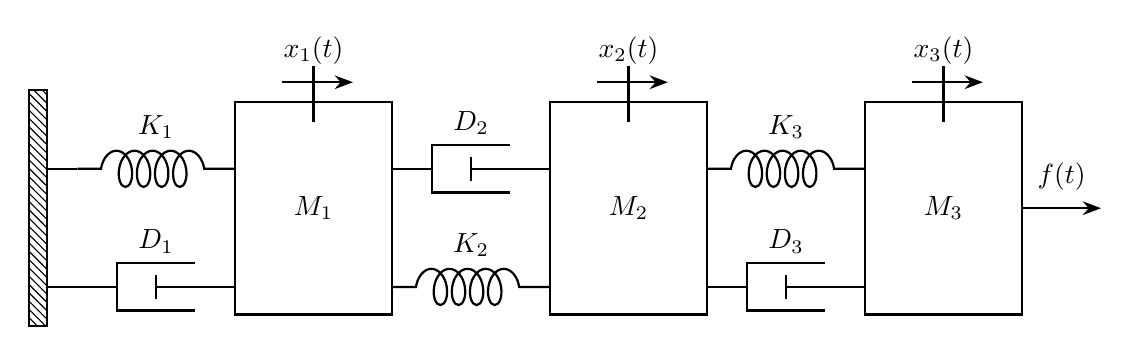
\begin{tikzpicture}[point/.style={coordinate}, >={Stealth}, thick]
        \node[wall] (W) at (-0.5,1) {};

        %damper
        \hdamper{(0,0)}{$D_1$}
        \hdamper{(4,1.5)}{$D_2$}
        \hdamper{(8,0)}{$D_3$}

        %spring
        \hspring{0,1.5}{$K_1$}
        \hspring{4,0}{$K_2$}
        \hspring{8,1.5}{$K_3$}
        
        %mass
        \tbody{3,1}{$M_1$}{$x_1(t)$}{M1};
        \tbody{7,1}{$M_2$}{$x_2(t)$}{M2};
        \tbody{11,1}{$M_3$}{$x_3(t)$}{M2};

    % f(t)
        \node at (12.5,1.4) {$f(t)$};
        \draw[->] (12,1) -- (13,1);

        
        \draw (-0.38,0) -- (0,0);
        \draw (-0.38,1.5) -- (0,1.5);
    \end{tikzpicture}
\end{center}

\noindent\rule{\textwidth}{1pt}

\vspace{12pt}

\noindent\textbf{\textit{Given:}}
\[
\begin{aligned}
M_1 &= 1\, \text{kg} & K_1 &= 6\, \text{N/m} & D_1 &= 3\, \text{N}\cdot\text{s/m} \\
M_2 &= 2\, \text{kg} & K_2 &= 4\, \text{N/m} & D_2 &= 2\, \text{N}\cdot\text{s/m} \\
M_3 &= 2\, \text{kg} & K_3 &= 4\, \text{N/m} & D_3 &= 2\, \text{N}\cdot\text{s/m}
\end{aligned}
\]

\vspace{12pt}

\noindent \textbf{\textit{Required:}}
\[
G(s) = \frac{X_1(s)}{F(s)}
\]

\vspace{12pt}

\noindent \textbf{\textit{Solution:}}

\vspace{12pt}

\noindent \textbf{Deriving the Equations of Motion}
\vspace{12pt}

\noindent We apply Newton's second law ($\sum F = ma$) to each mass, with the positive direction of motion to the right. 

\vspace{12pt}
{For Mass $M_1$:}
\begin{figure}[h!]
\centering
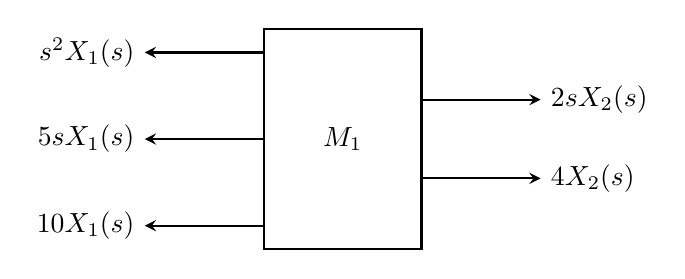
\begin{tikzpicture}[
    force/.style={->,>=stealth,thick}
]
    \node[draw, thick, minimum width=2cm, minimum height=2.8cm, label=center:$M_1$] (m1) {};

    \draw[force] ([yshift=1.1cm]m1.west) -- ++(-1.5,0) node[left] {$s^2X_1(s)$};
    \draw[force] ([yshift=0cm]m1.west) -- ++(-1.5,0) node[left] {$5sX_1(s)$};
    \draw[force] ([yshift=-1.1cm]m1.west) -- ++(-1.5,0) node[left] {$10X_1(s)$};

    \draw[force] ([yshift=0.5cm]m1.east) -- ++(1.5,0) node[right] {$2sX_2(s)$};
    \draw[force] ([yshift=-0.5cm]m1.east) -- ++(1.5,0) node[right] {$4X_2(s)$};
\end{tikzpicture}
\end{figure}

The resulting equation in the Laplace domain is:
\begin{equation}
(s^2 + 5s + 10)X_1(s) - (2s + 4)X_2(s) = 0 \tag{1}
\end{equation}

\vspace{12pt}
{For Mass $M_2$:}
\begin{figure}[h!]
\centering
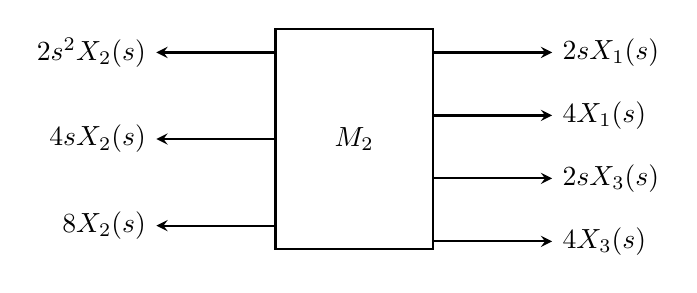
\begin{tikzpicture}[
    force/.style={->,>=stealth,thick}
]
    \node[draw, thick, minimum width=2cm, minimum height=2.8cm, label=center:$M_2$] (m2) {};

    \draw[force] ([yshift=1.1cm]m2.west) -- ++(-1.5,0) node[left] {$2s^2X_2(s)$};
    \draw[force] ([yshift=0cm]m2.west) -- ++(-1.5,0) node[left] {$4sX_2(s)$};
    \draw[force] ([yshift=-1.1cm]m2.west) -- ++(-1.5,0) node[left] {$8X_2(s)$};
    
    \draw[force] ([yshift=1.1cm]m2.east) -- ++(1.5,0) node[right] {$2sX_1(s)$};
    \draw[force] ([yshift=0.3cm]m2.east) -- ++(1.5,0) node[right] {$4X_1(s)$};
    \draw[force] ([yshift=-0.5cm]m2.east) -- ++(1.5,0) node[right] {$2sX_3(s)$};
    \draw[force] ([yshift=-1.3cm]m2.east) -- ++(1.5,0) node[right] {$4X_3(s)$};
\end{tikzpicture}
\end{figure}

The resulting equation in the Laplace domain is:
\begin{equation}
-(2s + 4)X_1(s) + (2s^2 + 4s + 8)X_2(s) - (2s + 4)X_3(s) = 0 \tag{2}
\end{equation}
\newpage

\vspace{12pt}
{For Mass $M_3$:}
\begin{figure}[h!]
\centering
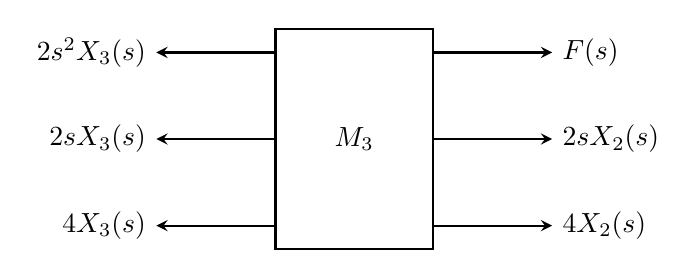
\begin{tikzpicture}[
    force/.style={->,>=stealth,thick}
]
    \node[draw, thick, minimum width=2cm, minimum height=2.8cm, label=center:$M_3$] (m3) {};

    \draw[force] ([yshift=1.1cm]m3.west) -- ++(-1.5,0) node[left] {$2s^2X_3(s)$};
    \draw[force] ([yshift=0cm]m3.west) -- ++(-1.5,0) node[left] {$2sX_3(s)$};
    \draw[force] ([yshift=-1.1cm]m3.west) -- ++(-1.5,0) node[left] {$4X_3(s)$};
    
    \draw[force] ([yshift=1.1cm]m3.east) -- ++(1.5,0) node[right] {$F(s)$};
    \draw[force] ([yshift=0cm]m3.east) -- ++(1.5,0) node[right] {$2sX_2(s)$};
    \draw[force] ([yshift=-1.1cm]m3.east) -- ++(1.5,0) node[right] {$4X_2(s)$};
\end{tikzpicture}
\end{figure}

The resulting equation in the Laplace domain is:
\begin{equation}
-(2s + 4)X_2(s) + (2s^2 + 2s + 4)X_3(s) = F(s) \tag{3}
\end{equation}

\noindent\textbf{Solving the System using Cramer's Rule}
\vspace{12pt}

The system can be expressed in matrix form $A\mathbf{x} = \mathbf{b}$:
$$
\begin{bmatrix}
s^2 + 5s + 10 & -(2s + 4) & 0 \\
-(2s + 4) & 2s^2 + 4s + 8 & -(2s + 4) \\
0 & -(2s + 4) & 2s^2 + 2s + 4
\end{bmatrix}
\begin{bmatrix}
X_1(s) \\
X_2(s) \\
X_3(s)
\end{bmatrix}
=
\begin{bmatrix}
0 \\
0 \\
F(s)
\end{bmatrix}
$$

The solution for $X_1(s)$ is $G(s) = \frac{X_1(s)}{F(s)} = \frac{\det(A_1)}{\det(A)} = \frac{\Delta_1}{\Delta}$.

\vspace{12pt}
\noindent\textbf{Calculating the Numerator Determinant, $\Delta_1$}:
$$ \Delta_1 = \det
\begin{bmatrix}
0 & -(2s + 4) & 0 \\
0 & 2s^2 + 4s + 8 & -(2s + 4) \\
F(s) & -(2s + 4) & 2s^2 + 2s + 4
\end{bmatrix}
= 4(s^2 + 4s + 4)F(s) $$

{Calculating the Denominator Determinant, $\Delta$}:
$$\Delta = \det(A) = 4(s^6 + 8s^5 + 30s^4 + 59s^3 + 74s^2 + 36s + 24)$$

{Constructing the Transfer Function}
$$G(s) = \frac{X_1(s)}{F(s)} = \frac{\Delta_1}{\Delta F(s)}$$

Expanding the denominator yields the simplified standard form:
\[
\boxed{
G(s) = \frac{s^2 + 4s + 4}{s^6 + 8s^5 + 30s^4 + 59s^3 + 74s^2 + 36s + 24}
}
\]

% Problem 7

\newpage
% command for new page 
  \setcounter{page}{2}  
\noindent\rule{\textwidth}{1pt}
\noindent\textbf{Problem 7} \hfill
\\For the translational mechanical system diagram shown below, determine the transfer function $G(s)=X_1(s)/F(s)$.

% P7 Figure
\begin{center}
    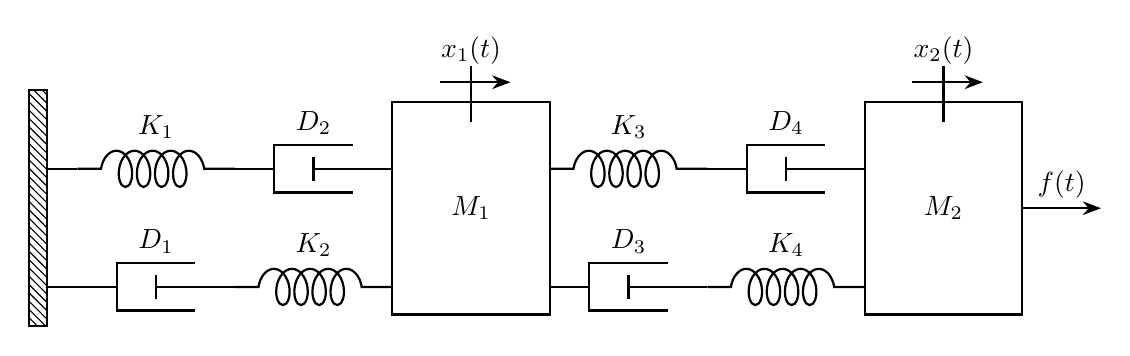
\begin{tikzpicture}[point/.style={coordinate}, >={Stealth}, thick]
        \node[wall] (W) at (-0.5,1) {};

        %damper
        \hdamper{(0,0)}{$D_1 $}
        \hdamper{(2,1.5)}{$D_2 $}
        \hdamper{(6,0)}{$D_3 $}
        \hdamper{(8,1.5)}{$D_4 $}

        %spring
        \hspring{0,1.5}{$K_1 $}
        \hspring{2,0}{$K_2 $}
        \hspring{6,1.5}{$K_3 $}
        \hspring{8,0}{$K_4 $}
        
        %mass
        \tbody{5,1}{$M_1$}{$x_1(t)$}{M1};
        \tbody{11,1}{$M_2$}{$x_2(t)$}{M2};

    % f(t)
        \node at (12.5,1.3) {$f(t)$};
        \draw[->] (12,1) -- (13,1);

        % \node at (x+.5,1.3) {\scriptsize $f(t)$};
        % \draw[->] (x,1) -- (x+1,1);
        
        \draw (-0.38,0) -- (0,0);
        \draw (-0.38,1.5) -- (0,1.5);
    \end{tikzpicture}
\end{center}

\noindent\rule{\textwidth}{1pt}

\vspace{12pt}

\noindent \textbf{\textit{Given:}}
\[
\begin{aligned}
M_1 &= 1\, \text{kg} & K_1 &= 2\, \text{N/m} & D_1 &= 2\, \text{N}\cdot\text{s/m} \\
M_2 &= 2\, \text{kg} & K_2 &= 3\, \text{N/m} & D_2 &= 1\, \text{N}\cdot\text{s/m} \\
& & K_3 &= 1\, \text{N/m} & D_3 &= 1\, \text{N}\cdot\text{s/m} \\
& & K_4 &= 1\, \text{N/m} & D_4 &= 1\, \text{N}\cdot\text{s/m}
\end{aligned}
\]

\vspace{12pt}

\noindent \textbf{\textit{Required:}}
\[
G(s) = \frac{X_1(s)}{F(s)}
\]

\vspace{12pt}

\noindent \textbf{\textit{Solution:}}

\vspace{12pt}

\noindent \textbf{Deriving the Equations of Motion}
\vspace{12pt}

\noindent We apply Newton's second law ($\sum F = ma$) to each mass, with the positive direction of motion to the right. 

\vspace{12pt}
{For Mass $M_1$:}
\begin{figure}[h!]
\centering
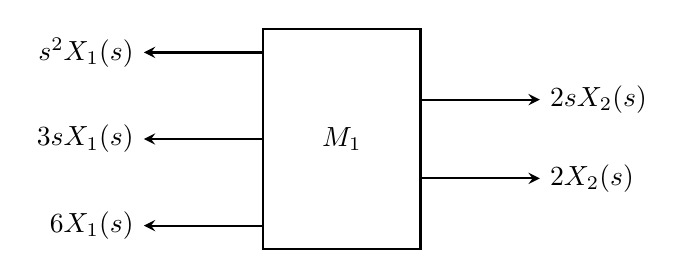
\begin{tikzpicture}[
    force/.style={->,>=stealth,thick}
]
    \node[draw, thick, minimum width=2cm, minimum height=2.8cm, label=center:$M_1$] (m1) {};

    \draw[force] ([yshift=1.1cm]m1.west) -- ++(-1.5,0) node[left] {$s^2X_1(s)$};
    \draw[force] ([yshift=0cm]m1.west) -- ++(-1.5,0) node[left] {$3sX_1(s)$};
    \draw[force] ([yshift=-1.1cm]m1.west) -- ++(-1.5,0) node[left] {$6X_1(s)$};

    \draw[force] ([yshift=0.5cm]m1.east) -- ++(1.5,0) node[right] {$2sX_2(s)$};
    \draw[force] ([yshift=-0.5cm]m1.east) -- ++(1.5,0) node[right] {$2X_2(s)$};
\end{tikzpicture}
\end{figure}

The resulting equation in the Laplace domain is:
\begin{equation}
(s^2 + 3s + 6)X_1(s) - (2s + 2)X_2(s) = 0 \tag{1}
\end{equation}

\vspace{12pt}
{For Mass $M_2$:}
\begin{figure}[h!]
\centering
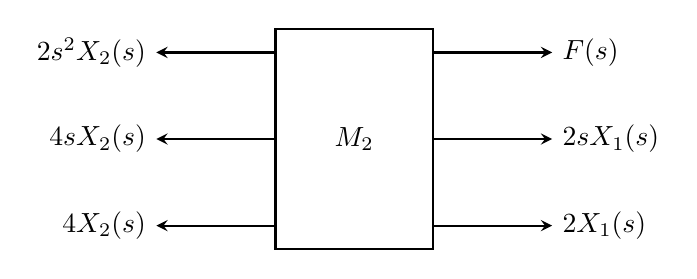
\begin{tikzpicture}[
    force/.style={->,>=stealth,thick}
]
    \node[draw, thick, minimum width=2cm, minimum height=2.8cm, label=center:$M_2$] (m2) {};

    \draw[force] ([yshift=1.1cm]m2.west) -- ++(-1.5,0) node[left] {$2s^2X_2(s)$};
    \draw[force] ([yshift=0cm]m2.west) -- ++(-1.5,0) node[left] {$4sX_2(s)$};
    \draw[force] ([yshift=-1.1cm]m2.west) -- ++(-1.5,0) node[left] {$4X_2(s)$};
    
    \draw[force] ([yshift=1.1cm]m2.east) -- ++(1.5,0) node[right] {$F(s)$};
    \draw[force] ([yshift=0cm]m2.east) -- ++(1.5,0) node[right] {$2sX_1(s)$};
    \draw[force] ([yshift=-1.1cm]m2.east) -- ++(1.5,0) node[right] {$2X_1(s)$};
\end{tikzpicture}
\end{figure}

The resulting equation in the Laplace domain is:
\begin{equation}
-(2s + 2)X_1(s) + (2s^2 + 4s + 4)X_2(s) = F(s) \tag{2}
\end{equation}

\newpage
\noindent\textbf{Solving the System using Cramer's Rule}
\vspace{12pt}

The system can be expressed in matrix form $A\mathbf{x} = \mathbf{b}$:
$$
\begin{bmatrix}
s^2 + 3s + 6 & -(2s + 2) \\
-(2s + 2) & 2s^2 + 4s + 4
\end{bmatrix}
\begin{bmatrix}
X_1(s) \\
X_2(s)
\end{bmatrix}
=
\begin{bmatrix}
0 \\
F(s)
\end{bmatrix}
$$

The solution for $X_1(s)$ is $G(s) = \frac{X_1(s)}{F(s)} = \frac{\det(A_1)}{\det(A)} = \frac{\Delta_1}{\Delta}$.

\vspace{12pt}
\noindent\textbf{Calculating the Numerator Determinant, $\Delta_1$}:
$$ \Delta_1 = \det
\begin{bmatrix}
0 & -(2s + 2) \\
F(s) & 2s^2 + 4s + 4
\end{bmatrix}
= (2s + 2)F(s) $$

{Calculating the Denominator Determinant, $\Delta$}:
$$\Delta = \det(A) = 2s^4 + 10s^3 + 26s^2 + 36s + 20$$

{Constructing the Transfer Function}
$$G(s) = \frac{X_1(s)}{F(s)} = \frac{\Delta_1}{\Delta F(s)}$$

Expanding the denominator yields the simplified standard form:
\[
\boxed{
G(s) = \frac{2s + 2}{2s^4 + 10s^3 + 26s^2 + 36s + 20}
}
\]

% Problem 8 - Translational Mechanical Transfer Function

\newpage
  \setcounter{page}{12}  
\noindent\rule{\textwidth}{1pt}
\noindent\textbf{Problem 8} \hfill
\\For the translational mechanical system diagram shown below, determine the transfer function $G(s)=X_1(s)/F(s)$.
% P8 Figure
\begin{center}
\resizebox{\textwidth}{!}{%
    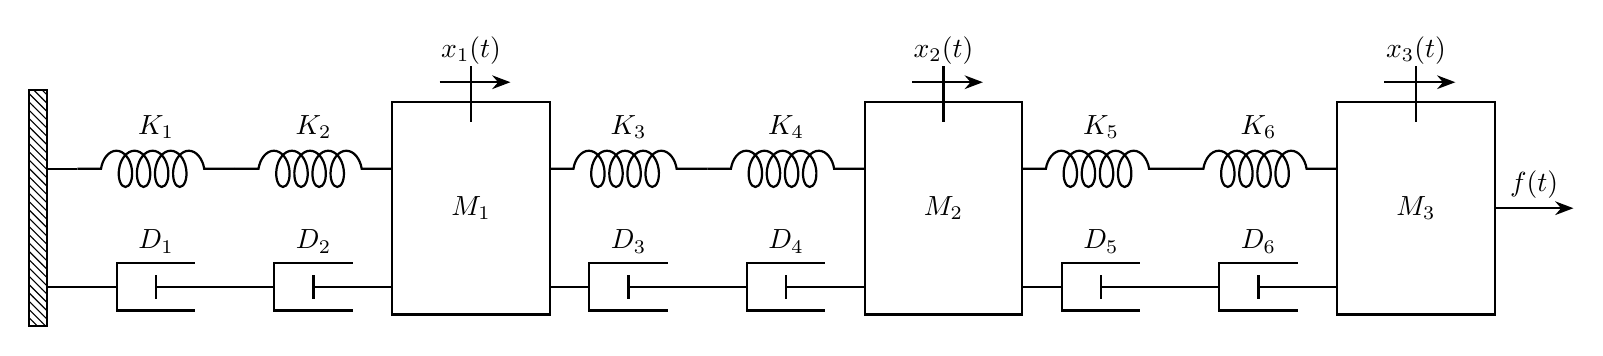
\begin{tikzpicture}[point/.style={coordinate}, >={Stealth}, thick]
        \node[wall] (W) at (-0.5,1) {};

        %damper
        \hdamper{(0,0)}{$D_1 $}
        \hdamper{(2,0)}{$D_2 $}
        \hdamper{(6,0)}{$D_3 $}
        \hdamper{(8,0)}{$D_4 $}
        \hdamper{(12,0)}{$D_5 $}
        \hdamper{(14,0)}{$D_6 $}

        %spring
        \hspring{0,1.5}{$K_1 $}
        \hspring{2,1.5}{$K_2 $}
        \hspring{6,1.5}{$K_3 $}
        \hspring{8,1.5}{$K_4 $}
        \hspring{12,1.5}{$K_5 $}
        \hspring{14,1.5}{$K_6 $}
        
        %mass
        \tbody{5,1}{$M_1$}{$x_1(t)$}{M1};
        \tbody{11,1}{$M_2$}{$x_2(t)$}{M2};
        \tbody{17,1}{$M_3$}{$x_3(t)$}{M2};

    % f(t)
        \node at (18.5,1.3) { $f(t)$};
        \draw[->] (18,1) -- (19,1);

        % \node at (x+.5,1.3) {\scriptsize $f(t)$};
        % \draw[->] (x,1) -- (x+1,1);
        
        \draw (-0.38,0) -- (0,0);
        \draw (-0.38,1.5) -- (0,1.5);
    \end{tikzpicture}
}
\end{center}
\noindent\rule{\textwidth}{1pt}

\vspace{12pt}

\noindent\textbf{\textit{Given:}}
\[
\begin{aligned}
M_1 &= 1\, \text{kg} & K_1 &= 2\, \text{N/m} & D_1 &= 1\, \text{N}\cdot\text{s/m} \\
M_2 &= 2\, \text{kg} & K_2 &= 2\, \text{N/m} & D_2 &= 1\, \text{N}\cdot\text{s/m} \\
M_3 &= 1\, \text{kg} & K_3 &= 1\, \text{N/m} & D_3 &= 1\, \text{N}\cdot\text{s/m} \\
& & K_4 &= 1\, \text{N/m} & D_4 &= 1\, \text{N}\cdot\text{s/m} \\
& & K_5 &= 1\, \text{N/m} & D_5 &= 1\, \text{N}\cdot\text{s/m} \\
& & K_6 &= 1\, \text{N/m} & D_6 &= 1\, \text{N}\cdot\text{s/m} \\
\end{aligned}
\]

\vspace{12pt}

\noindent \textbf{\textit{Required:}}
\[
G(s) = \frac{X_1(s)}{F(s)}
\]

\vspace{12pt}

\noindent \textbf{\textit{Solution:}}

\vspace{12pt}

\noindent \textbf{Deriving the Equations of Motion}
\vspace{12pt}

\noindent We apply Newton's second law ($\sum F = ma$) to each mass, with the positive direction of motion to the right. 

\vspace{12pt}
{For Mass $M_1$:}
\begin{figure}[h!]
\centering
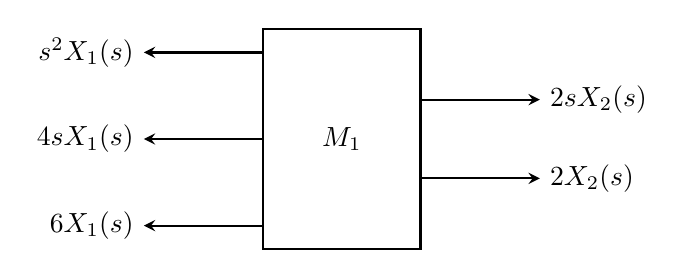
\begin{tikzpicture}[
    force/.style={->,>=stealth,thick}
]
    \node[draw, thick, minimum width=2cm, minimum height=2.8cm, label=center:$M_1$] (m1) {};

    \draw[force] ([yshift=1.1cm]m1.west) -- ++(-1.5,0) node[left] {$s^2X_1(s)$};
    \draw[force] ([yshift=0cm]m1.west) -- ++(-1.5,0) node[left] {$4sX_1(s)$};
    \draw[force] ([yshift=-1.1cm]m1.west) -- ++(-1.5,0) node[left] {$6X_1(s)$};

    \draw[force] ([yshift=0.5cm]m1.east) -- ++(1.5,0) node[right] {$2sX_2(s)$};
    \draw[force] ([yshift=-0.5cm]m1.east) -- ++(1.5,0) node[right] {$2X_2(s)$};
\end{tikzpicture}
\end{figure}

The resulting equation in the Laplace domain is:
\begin{equation}
(s^2 + 4s + 6)X_1(s) - (2s + 2)X_2(s) = 0 \tag{1}
\end{equation}

\vspace{12pt}
{For Mass $M_2$:}
\begin{figure}[h!]
\centering
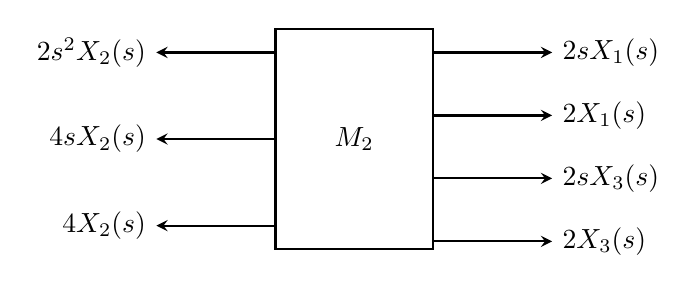
\begin{tikzpicture}[
    force/.style={->,>=stealth,thick}
]
    \node[draw, thick, minimum width=2cm, minimum height=2.8cm, label=center:$M_2$] (m2) {};

    \draw[force] ([yshift=1.1cm]m2.west) -- ++(-1.5,0) node[left] {$2s^2X_2(s)$};
    \draw[force] ([yshift=0cm]m2.west) -- ++(-1.5,0) node[left] {$4sX_2(s)$};
    \draw[force] ([yshift=-1.1cm]m2.west) -- ++(-1.5,0) node[left] {$4X_2(s)$};
    
    \draw[force] ([yshift=1.1cm]m2.east) -- ++(1.5,0) node[right] {$2sX_1(s)$};
    \draw[force] ([yshift=0.3cm]m2.east) -- ++(1.5,0) node[right] {$2X_1(s)$};
    \draw[force] ([yshift=-0.5cm]m2.east) -- ++(1.5,0) node[right] {$2sX_3(s)$};
    \draw[force] ([yshift=-1.3cm]m2.east) -- ++(1.5,0) node[right] {$2X_3(s)$};
\end{tikzpicture}
\end{figure}

The resulting equation in the Laplace domain is:
\begin{equation}
-(2s + 2)X_1(s) + (2s^2 + 4s + 4)X_2(s) - (2s + 2)X_3(s) = 0 \tag{2}
\end{equation}

\newpage

\vspace{12pt}
{For Mass $M_3$:}
\begin{figure}[h!]
\centering
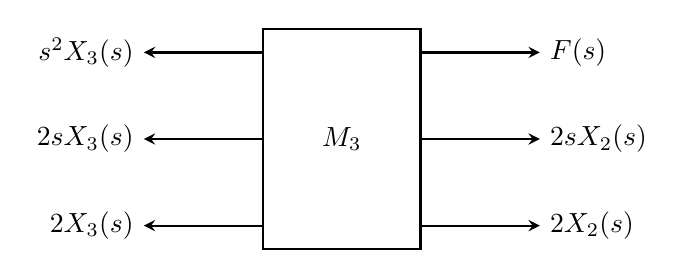
\begin{tikzpicture}[
    force/.style={->,>=stealth,thick}
]
    \node[draw, thick, minimum width=2cm, minimum height=2.8cm, label=center:$M_3$] (m3) {};

    \draw[force] ([yshift=1.1cm]m3.west) -- ++(-1.5,0) node[left] {$s^2X_3(s)$};
    \draw[force] ([yshift=0cm]m3.west) -- ++(-1.5,0) node[left] {$2sX_3(s)$};
    \draw[force] ([yshift=-1.1cm]m3.west) -- ++(-1.5,0) node[left] {$2X_3(s)$};
    
    \draw[force] ([yshift=1.1cm]m3.east) -- ++(1.5,0) node[right] {$F(s)$};
    \draw[force] ([yshift=0cm]m3.east) -- ++(1.5,0) node[right] {$2sX_2(s)$};
    \draw[force] ([yshift=-1.1cm]m3.east) -- ++(1.5,0) node[right] {$2X_2(s)$};
\end{tikzpicture}
\end{figure}

The resulting equation in the Laplace domain is:
\begin{equation}
-(2s + 2)X_2(s) + (s^2 + 2s + 2)X_3(s) = F(s) \tag{3}
\end{equation}

\noindent\textbf{Solving the System using Cramer's Rule}
\vspace{12pt}

The system can be expressed in matrix form $A\mathbf{x} = \mathbf{b}$:
$$
\begin{bmatrix}
s^2 + 4s + 6 & -(2s + 2) & 0 \\
-(2s + 2) & 2s^2 + 4s + 4 & -(2s + 2) \\
0 & -(2s + 2) & s^2 + 2s + 2
\end{bmatrix}
\begin{bmatrix}
X_1(s) \\
X_2(s) \\
X_3(s)
\end{bmatrix}
=
\begin{bmatrix}
0 \\
0 \\
F(s)
\end{bmatrix}
$$

The solution for $X_1(s)$ is $G(s) = \frac{X_1(s)}{F(s)} = \frac{\det(A_1)}{\det(A)} = \frac{\Delta_1}{\Delta}$.

\vspace{12pt}
\noindent\textbf{Calculating the Numerator Determinant, $\Delta_1$}:
$$ \Delta_1 = \det
\begin{bmatrix}
0 & -(2s + 2) & 0 \\
0 & 2s^2 + 4s + 4 & -(2s + 2) \\
F(s) & -(2s + 2) & s^2 + 2s + 2
\end{bmatrix}
= (s^2 + 4s + 4)F(s) $$

{Calculating the Denominator Determinant, $\Delta$}:
$$\Delta = \det(A) = s^6 + 8s^5 + 28s^4 + 52s^3 + 52s^2 + 24s + 8$$

{Constructing the Transfer Function}
$$G(s) = \frac{X_1(s)}{F(s)} = \frac{\Delta_1}{\Delta F(s)}$$

Expanding the denominator yields the simplified standard form:
\[
\boxed{
G(s) = \frac{s^2 + 4s + 4}{s^6 + 8s^5 + 28s^4 + 52s^3 + 52s^2 + 24s + 8}
}
\]


% Problem 9 - Translational Mechanical Transfer Function

\newpage
  \setcounter{page}{13}  
\noindent\rule{\textwidth}{1pt}
\noindent\textbf{Problem 9} \hfill
\\For the translational mechanical system diagram shown below, determine the transfer function $G(s)=X_1(s)/F(s)$.
% P6 Figure
% #1
% #4
\begin{center}
\resizebox{\textwidth}{!}{%
    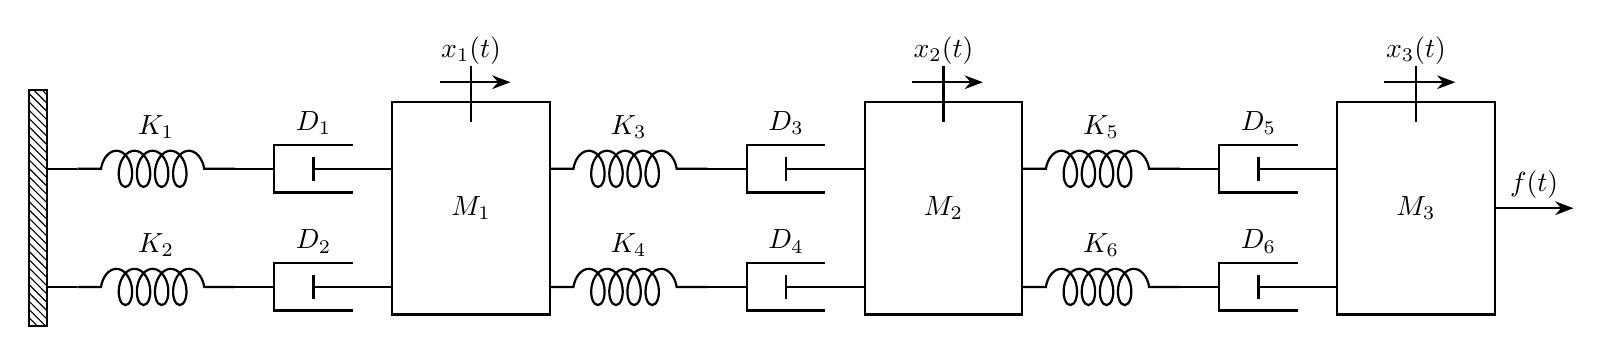
\begin{tikzpicture}[point/.style={coordinate}, >={Stealth}, thick]
        \node[wall] (W) at (-0.5,1) {};

        %damper
        \hdamper{(2,0)}{$D_2 $ }
        \hdamper{(2,1.5)}{$D_1 $ }
        \hdamper{(8,0)}{$D_4 $ }
        \hdamper{(8,1.5)}{$D_3 $ }
        \hdamper{(14,0)}{$D_6 $ }
        \hdamper{(14,1.5)}{$D_5 $ }

        %spring
        \hspring{0,0}{$K_2 $}
        \hspring{0,1.5}{$K_1 $}
        \hspring{6,0}{$K_4 $}
        \hspring{6,1.5}{$K_3 $}
        \hspring{12,0}{$K_6 $}
        \hspring{12,1.5}{$K_5 $}
        
        %mass
        \tbody{5,1}{$M_1$}{$x_1(t)$}{M1};
        \tbody{11,1}{$M_2$}{$x_2(t)$}{M2};
        \tbody{17,1}{$M_3$}{$x_3(t)$}{M3};

    % f(t)
        \node at (18.5,1.3) {$f(t)$};
        \draw[->] (18,1) -- (19,1);

        % \node at (x+.5,1.3) {$f(t)$};
        % \draw[->] (x,1) -- (x+1,1);
        
        \draw (-0.38,0) -- (0,0);
        \draw (-0.38,1.5) -- (0,1.5);
    \end{tikzpicture}
}
\end{center}
\noindent\rule{\textwidth}{1pt}

\vspace{12pt}

\noindent\textbf{\textit{Given:}}
\[
\begin{aligned}
M_1 &= 1\, \text{kg} & K_1 &= 1\, \text{N/m} & D_1 &= 1\, \text{N}\cdot\text{s/m} \\
M_2 &= 2\, \text{kg} & K_2 &= 1\, \text{N/m} & D_2 &= 1\, \text{N}\cdot\text{s/m} \\
M_3 &= 1\, \text{kg} & K_3 &= 1\, \text{N/m} & D_3 &= 1\, \text{N}\cdot\text{s/m} \\
& & K_4 &= 2\, \text{N/m} & D_4 &= 1\, \text{N}\cdot\text{s/m} \\
& & K_5 &= 1\, \text{N/m} & D_5 &= 1\, \text{N}\cdot\text{s/m} \\
& & K_6 &= 2\, \text{N/m} & D_6 &= 1\, \text{N}\cdot\text{s/m}
\end{aligned}
\]

\vspace{12pt}

\noindent \textbf{\textit{Required:}}
\[
G(s) = \frac{X_1(s)}{F(s)}
\]

\vspace{12pt}

\noindent \textbf{\textit{Solution:}}

\vspace{12pt}

\noindent \textbf{Deriving the Equations of Motion}
\vspace{12pt}

\noindent We apply Newton's second law ($\sum F = ma$) to each mass, with the positive direction of motion to the right. 

\vspace{12pt}
{For Mass $M_1$:}
\begin{figure}[h!]
\centering
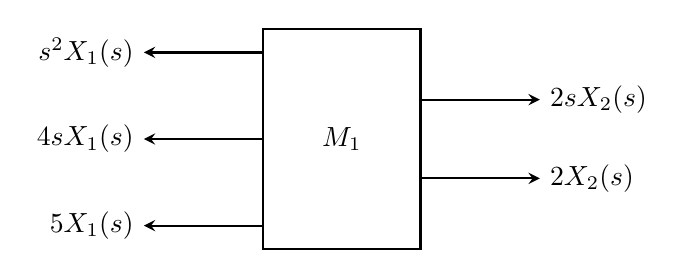
\begin{tikzpicture}[
    force/.style={->,>=stealth,thick}
]
    \node[draw, thick, minimum width=2cm, minimum height=2.8cm, label=center:$M_1$] (m1) {};

    \draw[force] ([yshift=1.1cm]m1.west) -- ++(-1.5,0) node[left] {$s^2X_1(s)$};
    \draw[force] ([yshift=0cm]m1.west) -- ++(-1.5,0) node[left] {$4sX_1(s)$};
    \draw[force] ([yshift=-1.1cm]m1.west) -- ++(-1.5,0) node[left] {$5X_1(s)$};

    \draw[force] ([yshift=0.5cm]m1.east) -- ++(1.5,0) node[right] {$2sX_2(s)$};
    \draw[force] ([yshift=-0.5cm]m1.east) -- ++(1.5,0) node[right] {$2X_2(s)$};
\end{tikzpicture}
\end{figure}

The resulting equation in the Laplace domain is:
\begin{equation}
(s^2 + 4s + 5)X_1(s) - (2s + 2)X_2(s) = 0 \tag{1}
\end{equation}

\vspace{12pt}
{For Mass $M_2$:}
\begin{figure}[h!]
\centering
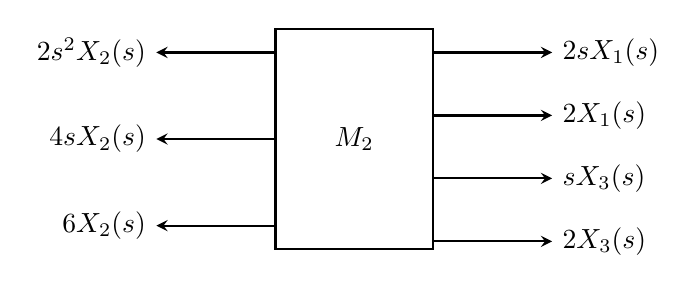
\begin{tikzpicture}[
    force/.style={->,>=stealth,thick}
]
    \node[draw, thick, minimum width=2cm, minimum height=2.8cm, label=center:$M_2$] (m2) {};

    \draw[force] ([yshift=1.1cm]m2.west) -- ++(-1.5,0) node[left] {$2s^2X_2(s)$};
    \draw[force] ([yshift=0cm]m2.west) -- ++(-1.5,0) node[left] {$4sX_2(s)$};
    \draw[force] ([yshift=-1.1cm]m2.west) -- ++(-1.5,0) node[left] {$6X_2(s)$};
    
    \draw[force] ([yshift=1.1cm]m2.east) -- ++(1.5,0) node[right] {$2sX_1(s)$};
    \draw[force] ([yshift=0.3cm]m2.east) -- ++(1.5,0) node[right] {$2X_1(s)$};
    \draw[force] ([yshift=-0.5cm]m2.east) -- ++(1.5,0) node[right] {$sX_3(s)$};
    \draw[force] ([yshift=-1.3cm]m2.east) -- ++(1.5,0) node[right] {$2X_3(s)$};
\end{tikzpicture}
\end{figure}

The resulting equation in the Laplace domain is:
\begin{equation}
-(2s + 2)X_1(s) + (2s^2 + 4s + 6)X_2(s) - (s + 2)X_3(s) = 0 \tag{2}
\end{equation}

\newpage

\vspace{12pt}
{For Mass $M_3$:}
\begin{figure}[h!]
\centering
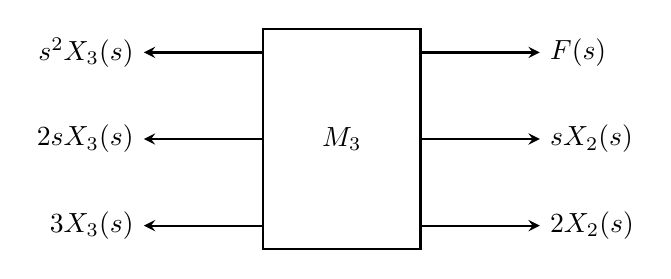
\begin{tikzpicture}[
    force/.style={->,>=stealth,thick}
]
    \node[draw, thick, minimum width=2cm, minimum height=2.8cm, label=center:$M_3$] (m3) {};

    \draw[force] ([yshift=1.1cm]m3.west) -- ++(-1.5,0) node[left] {$s^2X_3(s)$};
    \draw[force] ([yshift=0cm]m3.west) -- ++(-1.5,0) node[left] {$2sX_3(s)$};
    \draw[force] ([yshift=-1.1cm]m3.west) -- ++(-1.5,0) node[left] {$3X_3(s)$};
    
    \draw[force] ([yshift=1.1cm]m3.east) -- ++(1.5,0) node[right] {$F(s)$};
    \draw[force] ([yshift=0cm]m3.east) -- ++(1.5,0) node[right] {$sX_2(s)$};
    \draw[force] ([yshift=-1.1cm]m3.east) -- ++(1.5,0) node[right] {$2X_2(s)$};
\end{tikzpicture}
\end{figure}

The resulting equation in the Laplace domain is:
\begin{equation}
-(s + 2)X_2(s) + (s^2 + 2s + 3)X_3(s) = F(s) \tag{3}
\end{equation}

\noindent\textbf{Solving the System using Cramer's Rule}
\vspace{12pt}

The system can be expressed in matrix form $A\mathbf{x} = \mathbf{b}$:
$$
\begin{bmatrix}
s^2 + 4s + 5 & -(2s + 2) & 0 \\
-(2s + 2) & 2s^2 + 4s + 6 & -(s + 2) \\
0 & -(s + 2) & s^2 + 2s + 3
\end{bmatrix}
\begin{bmatrix}
X_1(s) \\
X_2(s) \\
X_3(s)
\end{bmatrix}
=
\begin{bmatrix}
0 \\
0 \\
F(s)
\end{bmatrix}
$$

The solution for $X_1(s)$ is $G(s) = \frac{X_1(s)}{F(s)} = \frac{\det(A_1)}{\det(A)} = \frac{\Delta_1}{\Delta}$.

\vspace{12pt}
\noindent\textbf{Calculating the Numerator Determinant, $\Delta_1$}:
$$ \Delta_1 = \det
\begin{bmatrix}
0 & -(2s + 2) & 0 \\
0 & 2s^2 + 4s + 6 & -(s + 2) \\
F(s) & -(s + 2) & s^2 + 2s + 3
\end{bmatrix}
= (s + 2)F(s) $$

{Calculating the Denominator Determinant, $\Delta$}:
$$\Delta = \det(A) = s^6 + 8s^5 + 25s^4 + 46s^3 + 49s^2 + 26s + 10$$

{Constructing the Transfer Function}
$$G(s) = \frac{X_1(s)}{F(s)} = \frac{\Delta_1}{\Delta F(s)}$$

Expanding the denominator yields the simplified standard form:
\[
\boxed{
G(s) = \frac{s + 2}{s^6 + 8s^5 + 25s^4 + 46s^3 + 49s^2 + 26s + 10}
}
\]
% Problem 10 - Translational Mechanical Transfer Function

\newpage
  \setcounter{page}{14}  
\noindent\rule{\textwidth}{1pt}
\noindent\textbf{Problem 10} \hfill
\\For the translational mechanical system diagram shown below, determine the transfer function $G(s)=X_1(s)/F(s)$.
% P6 Figure
% #1
% #5/6
\begin{center}
\resizebox{\textwidth}{!}{%
    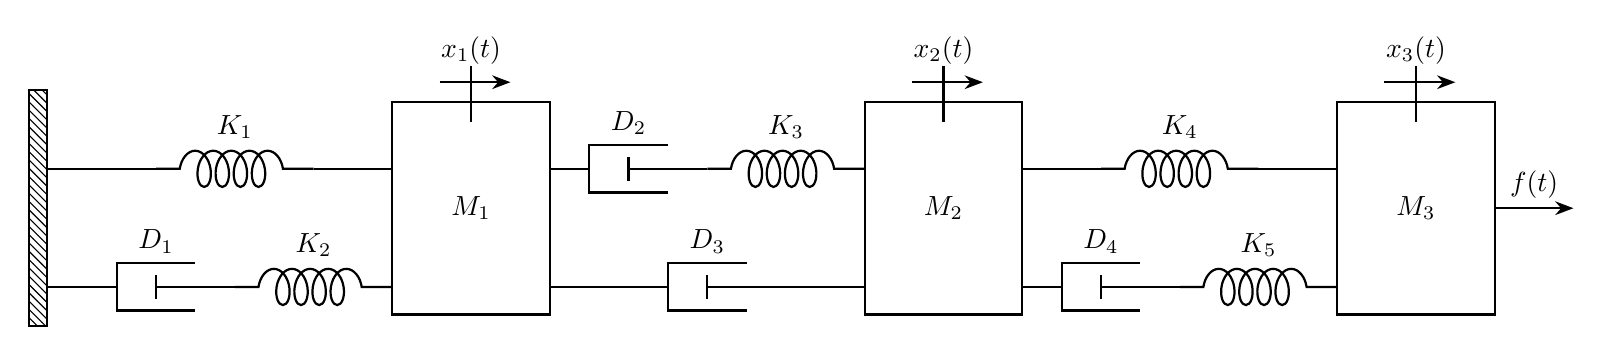
\begin{tikzpicture}[point/.style={coordinate}, >={Stealth}, thick]
        \node[wall] (W) at (-0.5,1) {};

        %damper
        \hdamper{(0,0)}{$D_1$}
        \hdamper{(7,0)}{$D_3$}
        \hdamper{(6,1.5)}{$D_2$}
        \hdamper{(12,0)}{$D_4$}

        %spring
        \hspring{1,1.5}{$K_1$}
        \hspring{2,0}{$K_2$}
        \hspring{8,1.5}{$K_3$}
        \hspring{13,1.5}{$K_4$}
        \hspring{14,0}{$K_5$}
        
        %mass
        \tbody{5,1}{$M_1$}{$x_1(t)$}{M1};
        \tbody{11,1}{$M_2$}{$x_2(t)$}{M2};
        \tbody{17,1}{$M_3$}{$x_3(t)$}{M2};

    % f(t)
        \node at (18.5,1.3) {$f(t)$};
        \draw[->] (18,1) -- (19,1);

        % \node at (x+.5,1.3) {$f(t)$};
        % \draw[->] (x,1) -- (x+1,1);
        
        \draw (-0.38,0) -- (0,0);
        \draw (-0.38,1.5) -- (1,1.5);
        \draw (3,1.5) -- (4,1.5);
        \draw (6,0) -- (7,0);
        \draw (9,0) -- (10,0);
        \draw (12,1.5) -- (13,1.5);
        \draw (15,1.5) -- (16,1.5);
        
    \end{tikzpicture}
}
\end{center}

\noindent\rule{\textwidth}{1pt}

\vspace{12pt}

\noindent\textbf{\textit{Given:}}
\[
\begin{aligned}
M_1 &= 2\, \text{kg} & K_1 &= 4\, \text{N/m} & D_1 &= 6\, \text{N}\cdot\text{s/m} \\
M_2 &= 1\, \text{kg} & K_2 &= 5\, \text{N/m} & D_2 &= 2\, \text{N}\cdot\text{s/m} \\
M_3 &= 1\, \text{kg} & K_3 &= 3\, \text{N/m} & D_3 &= 1\, \text{N}\cdot\text{s/m} \\
& & K_4 &= 2\, \text{N/m} & D_4 &= 4\, \text{N}\cdot\text{s/m} \\
& & K_5 &= 1\, \text{N/m} & & 
\end{aligned}
\]

\vspace{12pt}

\noindent \textbf{\textit{Required:}}
\[
G(s) = \frac{X_1(s)}{F(s)}
\]

\vspace{12pt}

\noindent \textbf{\textit{Solution:}}

\vspace{12pt}

\noindent \textbf{Deriving the Equations of Motion}
\vspace{12pt}

\noindent We apply Newton's second law ($\sum F = ma$) to each mass, with the positive direction of motion to the right. 

\vspace{12pt}
{For Mass $M_1$:}
\begin{figure}[h!]
\centering
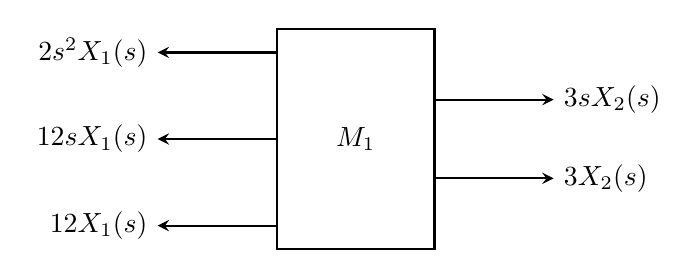
\begin{tikzpicture}[
    force/.style={->,>=stealth,thick}
]
    \node[draw, thick, minimum width=2cm, minimum height=2.8cm, label=center:$M_1$] (m1) {};

    \draw[force] ([yshift=1.1cm]m1.west) -- ++(-1.5,0) node[left] {$2s^2X_1(s)$};
    \draw[force] ([yshift=0cm]m1.west) -- ++(-1.5,0) node[left] {$12sX_1(s)$};
    \draw[force] ([yshift=-1.1cm]m1.west) -- ++(-1.5,0) node[left] {$12X_1(s)$};

    \draw[force] ([yshift=0.5cm]m1.east) -- ++(1.5,0) node[right] {$3sX_2(s)$};
    \draw[force] ([yshift=-0.5cm]m1.east) -- ++(1.5,0) node[right] {$3X_2(s)$};
\end{tikzpicture}
\end{figure}

The resulting equation in the Laplace domain is:
\begin{equation}
(2s^2 + 12s + 12)X_1(s) - (3s + 3)X_2(s) = 0 \tag{1}
\end{equation}

\vspace{12pt}
{For Mass $M_2$:}
\begin{figure}[h!]
\centering
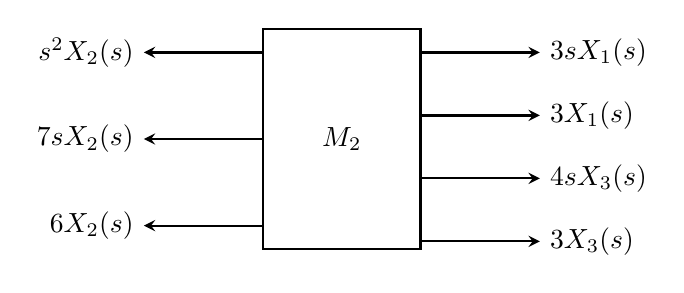
\begin{tikzpicture}[
    force/.style={->,>=stealth,thick}
]
    \node[draw, thick, minimum width=2cm, minimum height=2.8cm, label=center:$M_2$] (m2) {};

    \draw[force] ([yshift=1.1cm]m2.west) -- ++(-1.5,0) node[left] {$s^2X_2(s)$};
    \draw[force] ([yshift=0cm]m2.west) -- ++(-1.5,0) node[left] {$7sX_2(s)$};
    \draw[force] ([yshift=-1.1cm]m2.west) -- ++(-1.5,0) node[left] {$6X_2(s)$};
    
    \draw[force] ([yshift=1.1cm]m2.east) -- ++(1.5,0) node[right] {$3sX_1(s)$};
    \draw[force] ([yshift=0.3cm]m2.east) -- ++(1.5,0) node[right] {$3X_1(s)$};
    \draw[force] ([yshift=-0.5cm]m2.east) -- ++(1.5,0) node[right] {$4sX_3(s)$};
    \draw[force] ([yshift=-1.3cm]m2.east) -- ++(1.5,0) node[right] {$3X_3(s)$};
\end{tikzpicture}
\end{figure}

The resulting equation in the Laplace domain is:
\begin{equation}
-(3s + 3)X_1(s) + (s^2 + 7s + 6)X_2(s) - (4s + 3)X_3(s) = 0 \tag{2}
\end{equation}

\newpage

\vspace{12pt}
{For Mass $M_3$:}
\begin{figure}[h!]
\centering
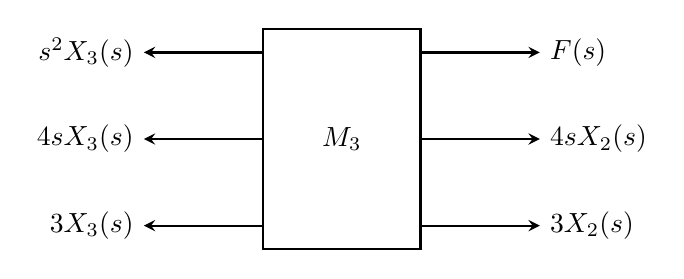
\begin{tikzpicture}[
    force/.style={->,>=stealth,thick}
]
    \node[draw, thick, minimum width=2cm, minimum height=2.8cm, label=center:$M_3$] (m3) {};

    \draw[force] ([yshift=1.1cm]m3.west) -- ++(-1.5,0) node[left] {$s^2X_3(s)$};
    \draw[force] ([yshift=0cm]m3.west) -- ++(-1.5,0) node[left] {$4sX_3(s)$};
    \draw[force] ([yshift=-1.1cm]m3.west) -- ++(-1.5,0) node[left] {$3X_3(s)$};
    
    \draw[force] ([yshift=1.1cm]m3.east) -- ++(1.5,0) node[right] {$F(s)$};
    \draw[force] ([yshift=0cm]m3.east) -- ++(1.5,0) node[right] {$4sX_2(s)$};
    \draw[force] ([yshift=-1.1cm]m3.east) -- ++(1.5,0) node[right] {$3X_2(s)$};
\end{tikzpicture}
\end{figure}

The resulting equation in the Laplace domain is:
\begin{equation}
-(4s + 3)X_2(s) + (s^2 + 4s + 3)X_3(s) = F(s) \tag{3}
\end{equation}

\noindent\textbf{Solving the System using Cramer's Rule}
\vspace{12pt}

The system can be expressed in matrix form $A\mathbf{x} = \mathbf{b}$:
$$
\begin{bmatrix}
2s^2 + 12s + 12 & -(3s + 3) & 0 \\
-(3s + 3) & s^2 + 7s + 6 & -(4s + 3) \\
0 & -(4s + 3) & s^2 + 4s + 3
\end{bmatrix}
\begin{bmatrix}
X_1(s) \\
X_2(s) \\
X_3(s)
\end{bmatrix}
=
\begin{bmatrix}
0 \\
0 \\
F(s)
\end{bmatrix}
$$

The solution for $X_1(s)$ is $G(s) = \frac{X_1(s)}{F(s)} = \frac{\det(A_1)}{\det(A)} = \frac{\Delta_1}{\Delta}$.

\vspace{12pt}
\noindent\textbf{Calculating the Numerator Determinant, $\Delta_1$}:
$$ \Delta_1 = \det
\begin{bmatrix}
0 & -(3s + 3) & 0 \\
0 & s^2 + 7s + 6 & -(4s + 3) \\
F(s) & -(4s + 3) & s^2 + 4s + 3
\end{bmatrix}
= (3s + 3)(4s + 3)F(s) $$

{Calculating the Denominator Determinant, $\Delta$}:
$$\Delta = \det(A) = (2s^2 + 12s + 12)\left[(s^2 + 7s + 6)(s^2 + 4s + 3) + (3 + 4s)(3 + 3s)\right]$$

{Constructing the Transfer Function}
$$G(s) = \frac{X_1(s)}{F(s)} = \frac{\Delta_1}{\Delta F(s)}$$

Expanding the denominator yields the simplified standard form:
\[
\boxed{
G(s) = \frac{(3s + 3)(4s + 3)}{(2s^2 + 12s + 12)\left[(s^2 + 7s + 6)(s^2 + 4s + 3) + (3 + 4s)(3 + 3s)\right]}
}
\]

% Problem 11 - Translational Mechanical Transfer Function

\newpage
  \setcounter{page}{16}  
\noindent\rule{\textwidth}{1pt}
\noindent\textbf{Problem 11} \hfill
\\For the translational mechanical system diagram shown below, determine the transfer function $G(s)=X_1(s)/F(s)$.
% P6 Figure
% #1
% #7
\begin{center}
\resizebox{\textwidth}{!}{%
    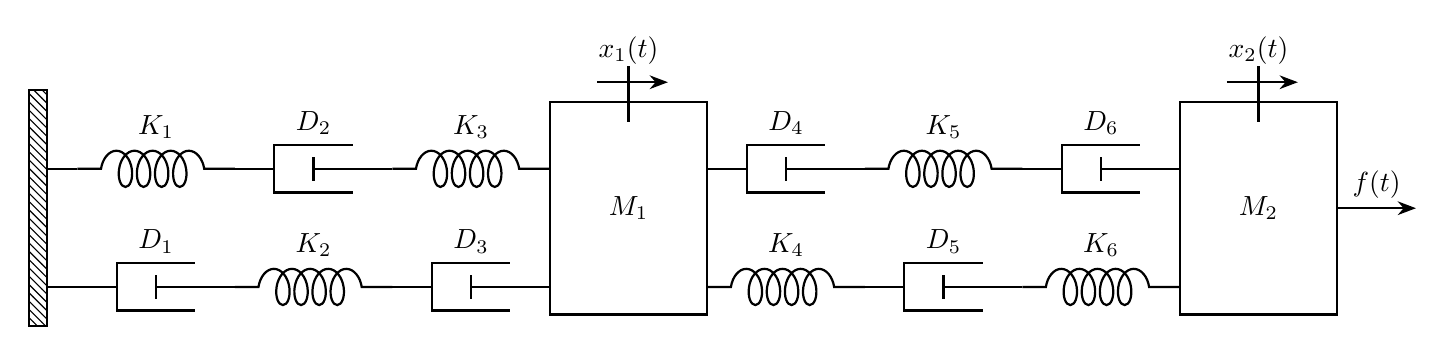
\begin{tikzpicture}[point/.style={coordinate}, >={Stealth}, thick]
        \node[wall] (W) at (-0.5,1) {};

        %damper
        \hdamper{(0,0)}{$D_1$}
        \hdamper{(2,1.5)}{$D_2$}
        \hdamper{(4,0)}{$D_3$}
        \hdamper{(8,1.5)}{$D_4$}
        \hdamper{(10,0)}{$D_5$}
        \hdamper{(12,1.5)}{$D_6$}

        %spring
        \hspring{0,1.5}{$K_1$}
        \hspring{2,0}{$K_2$}
        \hspring{4,1.5}{$K_3$}
        \hspring{8,0}{$K_4$}
        \hspring{10,1.5}{$K_5$}
        \hspring{12,0}{$K_6$}
        
        %mass
        \tbody{7,1}{$M_1 $}{$x_1(t)$}{M1};
        \tbody{15,1}{$M_2 $}{$x_2(t)$}{M2};

    % f(t)
        \node at (16.5,1.3) { $f(t)$};
        \draw[->] (16,1) -- (17,1);

        % \node at (x+.5,1.3) { $f(t)$};
        % \draw[->] (x,1) -- (x+1,1);
        
        \draw (-0.38,0) -- (0,0);
        \draw (-0.38,1.5) -- (0,1.5);
        
    \end{tikzpicture}
}
\end{center}
\noindent\rule{\textwidth}{1pt}

\vspace{12pt}

\noindent\textbf{\textit{Given:}}
\[
\begin{aligned}
M_1 &= 1\, \text{kg} & K_1 &= 1\, \text{N/m} & D_1 &= 1\, \text{N}\cdot\text{s/m} \\
M_2 &= 1\, \text{kg} & K_2 &= 1\, \text{N/m} & D_2 &= 1\, \text{N}\cdot\text{s/m} \\
& & K_3 &= 1\, \text{N/m} & D_3 &= 1\, \text{N}\cdot\text{s/m} \\
& & K_4 &= 1\, \text{N/m} & D_4 &= 1\, \text{N}\cdot\text{s/m} \\
& & K_5 &= 1\, \text{N/m} & D_5 &= 1\, \text{N}\cdot\text{s/m} \\
& & K_6 &= 1\, \text{N/m} & D_6 &= 1\, \text{N}\cdot\text{s/m}
\end{aligned}
\]

\vspace{12pt}

\noindent \textbf{\textit{Required:}}
\[
G(s) = \frac{X_1(s)}{F(s)}
\]

\vspace{12pt}

\noindent \textbf{\textit{Solution:}}

\vspace{12pt}

\noindent \textbf{Deriving the Equations of Motion}
\vspace{12pt}

\noindent We apply Newton's second law ($\sum F = ma$) to each mass, with the positive direction of motion to the right. 

\vspace{12pt}
{For Mass $M_1$:}
\begin{figure}[h!]
\centering
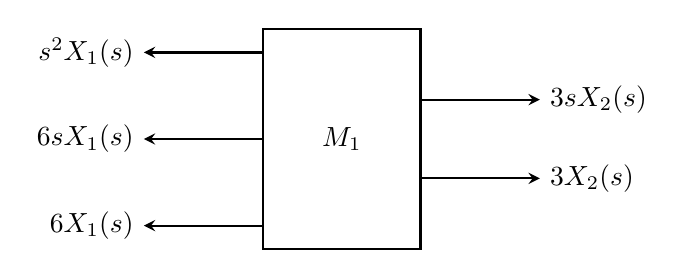
\begin{tikzpicture}[
    force/.style={->,>=stealth,thick}
]
    \node[draw, thick, minimum width=2cm, minimum height=2.8cm, label=center:$M_1$] (m1) {};

    \draw[force] ([yshift=1.1cm]m1.west) -- ++(-1.5,0) node[left] {$s^2X_1(s)$};
    \draw[force] ([yshift=0cm]m1.west) -- ++(-1.5,0) node[left] {$6sX_1(s)$};
    \draw[force] ([yshift=-1.1cm]m1.west) -- ++(-1.5,0) node[left] {$6X_1(s)$};

    \draw[force] ([yshift=0.5cm]m1.east) -- ++(1.5,0) node[right] {$3sX_2(s)$};
    \draw[force] ([yshift=-0.5cm]m1.east) -- ++(1.5,0) node[right] {$3X_2(s)$};
\end{tikzpicture}
\end{figure}

The resulting equation in the Laplace domain is:
\begin{equation}
(s^2 + 6s + 6)X_1(s) - (3s + 3)X_2(s) = 0 \tag{1}
\end{equation}

\vspace{12pt}
{For Mass $M_2$:}
\begin{figure}[h!]
\centering
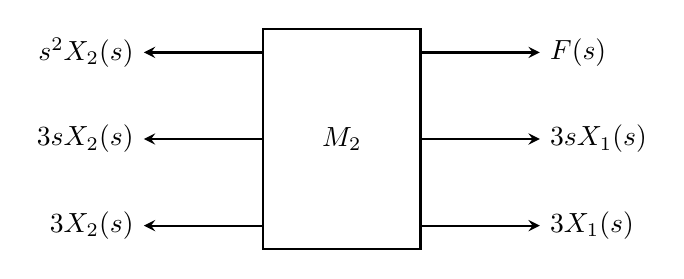
\begin{tikzpicture}[
    force/.style={->,>=stealth,thick}
]
    \node[draw, thick, minimum width=2cm, minimum height=2.8cm, label=center:$M_2$] (m2) {};

    \draw[force] ([yshift=1.1cm]m2.west) -- ++(-1.5,0) node[left] {$s^2X_2(s)$};
    \draw[force] ([yshift=0cm]m2.west) -- ++(-1.5,0) node[left] {$3sX_2(s)$};
    \draw[force] ([yshift=-1.1cm]m2.west) -- ++(-1.5,0) node[left] {$3X_2(s)$};
    
    \draw[force] ([yshift=1.1cm]m2.east) -- ++(1.5,0) node[right] {$F(s)$};
    \draw[force] ([yshift=0cm]m2.east) -- ++(1.5,0) node[right] {$3sX_1(s)$};
    \draw[force] ([yshift=-1.1cm]m2.east) -- ++(1.5,0) node[right] {$3X_1(s)$};
\end{tikzpicture}
\end{figure}

The resulting equation in the Laplace domain is:
\begin{equation}
-(3s + 3)X_1(s) + (s^2 + 3s + 3)X_2(s) = F(s) \tag{2}
\end{equation}

\newpage
\noindent\textbf{Solving the System using Cramer's Rule}
\vspace{12pt}

The system can be expressed in matrix form $A\mathbf{x} = \mathbf{b}$:
$$
\begin{bmatrix}
s^2 + 6s + 6 & -(3s + 3) \\
-(3s + 3) & s^2 + 3s + 3
\end{bmatrix}
\begin{bmatrix}
X_1(s) \\
X_2(s)
\end{bmatrix}
=
\begin{bmatrix}
0 \\
F(s)
\end{bmatrix}
$$

The solution for $X_1(s)$ is $G(s) = \frac{X_1(s)}{F(s)} = \frac{\det(A_1)}{\det(A)} = \frac{\Delta_1}{\Delta}$.

\vspace{12pt}
\noindent\textbf{Calculating the Numerator Determinant, $\Delta_1$}:
$$ \Delta_1 = \det
\begin{bmatrix}
0 & -(3s + 3) \\
F(s) & s^2 + 3s + 3
\end{bmatrix}
= (3s + 3)F(s) $$

{Calculating the Denominator Determinant, $\Delta$}:
$$\Delta = \det(A) = s^4 + 9s^3 + 18s^2 + 18s + 9$$

{Constructing the Transfer Function}
$$G(s) = \frac{X_1(s)}{F(s)} = \frac{\Delta_1}{\Delta F(s)}$$

Expanding the denominator yields the simplified standard form:
\[
\boxed{
G(s) = \frac{3s + 3}{s^4 + 9s^3 + 18s^2 + 18s + 9}
}
\]

% Problem 12 - Translational Mechanical Transfer Function

\newpage
  \setcounter{page}{18}  
\noindent\rule{\textwidth}{1pt}
\noindent\textbf{Problem 12} \hfill
\\For the translational mechanical system diagram shown below, determine the transfer function $G(s)=X_1(s)/F(s)$.
% P6 Figure
% #1
% #8
\begin{center}
\resizebox{\textwidth}{!}{%
    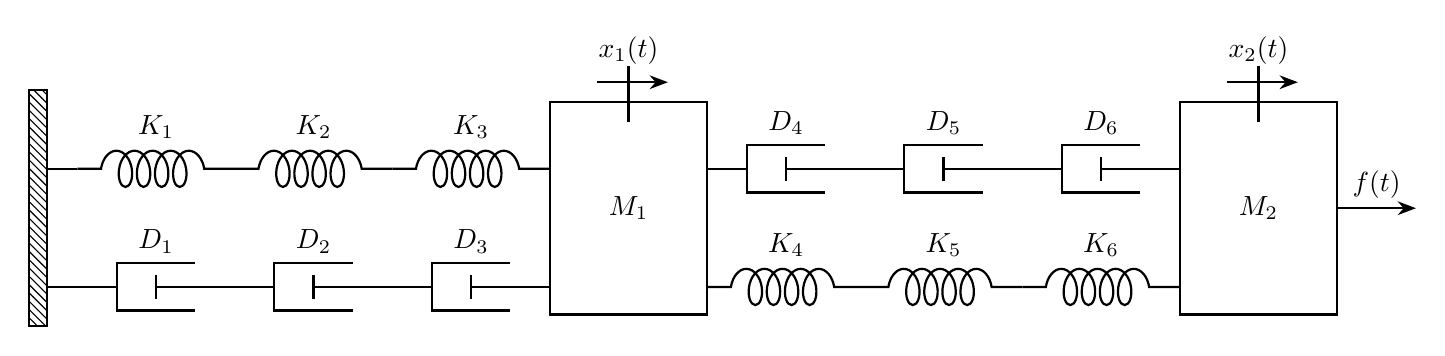
\begin{tikzpicture}[point/.style={coordinate}, >={Stealth}, thick]
        \node[wall] (W) at (-0.5,1) {};

        %damper
        \hdamper{(0,0)}{$D_1 $}
        \hdamper{(2,0)}{$D_2 $}
        \hdamper{(4,0)}{$D_3 $}
        \hdamper{(8,1.5)}{$D_4 $}
        \hdamper{(10,1.5)}{$D_5 $}
        \hdamper{(12,1.5)}{$D_6 $}

        %spring
        \hspring{0,1.5}{$K_1 $}
        \hspring{2,1.5}{$K_2 $}
        \hspring{4,1.5}{$K_3 $}
        \hspring{8,0}{$K_4 $}
        \hspring{10,0}{$K_5 $}
        \hspring{12,0}{$K_6 $}
        
        %mass
        \tbody{7,1}{$M_1$}{$x_1(t)$}{M1};
        \tbody{15,1}{$M_2$}{$x_2(t)$}{M2};

    % f(t)
        \node at (16.5,1.3) { $f(t)$};
        \draw[->] (16,1) -- (17,1);

        % \node at (x+.5,1.3) { $f(t)$};
        % \draw[->] (x,1) -- (x+1,1);
        
        \draw (-0.38,0) -- (0,0);
        \draw (-0.38,1.5) -- (0,1.5);
        
    \end{tikzpicture}
}
\end{center}

\noindent\rule{\textwidth}{1pt}

\vspace{12pt}

\noindent\textbf{\textit{Given:}}
\[
\begin{aligned}
M_1 &= 2\, \text{kg} & K_1 &= 1\, \text{N/m} & D_1 &= 1\, \text{N}\cdot\text{s/m} \\
M_2 &= 1\, \text{kg} & K_2 &= 1\, \text{N/m} & D_2 &= 1\, \text{N}\cdot\text{s/m} \\
& & K_3 &= 1\, \text{N/m} & D_3 &= 1\, \text{N}\cdot\text{s/m} \\
& & K_4 &= 1\, \text{N/m} & D_4 &= 1\, \text{N}\cdot\text{s/m} \\
& & K_5 &= 1\, \text{N/m} & D_5 &= 1\, \text{N}\cdot\text{s/m} \\
& & K_6 &= 1\, \text{N/m} & D_6 &= 1\, \text{N}\cdot\text{s/m}
\end{aligned}
\]

\vspace{12pt}

\noindent \textbf{\textit{Required:}}
\[
G(s) = \frac{X_1(s)}{F(s)}
\]

\vspace{12pt}

\noindent \textbf{\textit{Solution:}}

\vspace{12pt}

\noindent \textbf{Deriving the Equations of Motion}
\vspace{12pt}

\noindent We apply Newton's second law ($\sum F = ma$) to each mass, with the positive direction of motion to the right. 

\vspace{12pt}
{For Mass $M_1$:}
\begin{figure}[h!]
\centering
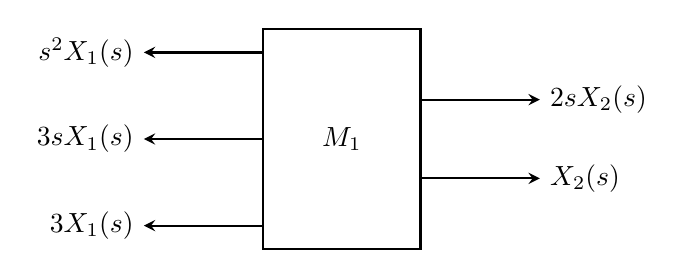
\begin{tikzpicture}[
    force/.style={->,>=stealth,thick}
]
    \node[draw, thick, minimum width=2cm, minimum height=2.8cm, label=center:$M_1$] (m1) {};

    \draw[force] ([yshift=1.1cm]m1.west) -- ++(-1.5,0) node[left] {$s^2X_1(s)$};
    \draw[force] ([yshift=0cm]m1.west) -- ++(-1.5,0) node[left] {$3sX_1(s)$};
    \draw[force] ([yshift=-1.1cm]m1.west) -- ++(-1.5,0) node[left] {$3X_1(s)$};

    \draw[force] ([yshift=0.5cm]m1.east) -- ++(1.5,0) node[right] {$2sX_2(s)$};
    \draw[force] ([yshift=-0.5cm]m1.east) -- ++(1.5,0) node[right] {$X_2(s)$};
\end{tikzpicture}
\end{figure}

The resulting equation in the Laplace domain is:
\begin{equation}
(s^2 + 3s + 3)X_1(s) - (2s + 1)X_2(s) = 0 \tag{1}
\end{equation}

\vspace{12pt}
{For Mass $M_2$:}
\begin{figure}[h!]
\centering
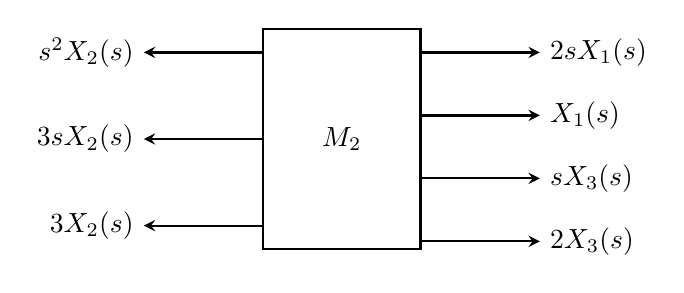
\begin{tikzpicture}[
    force/.style={->,>=stealth,thick}
]
    \node[draw, thick, minimum width=2cm, minimum height=2.8cm, label=center:$M_2$] (m2) {};

    \draw[force] ([yshift=1.1cm]m2.west) -- ++(-1.5,0) node[left] {$s^2X_2(s)$};
    \draw[force] ([yshift=0cm]m2.west) -- ++(-1.5,0) node[left] {$3sX_2(s)$};
    \draw[force] ([yshift=-1.1cm]m2.west) -- ++(-1.5,0) node[left] {$3X_2(s)$};
    
    \draw[force] ([yshift=1.1cm]m2.east) -- ++(1.5,0) node[right] {$2sX_1(s)$};
    \draw[force] ([yshift=0.3cm]m2.east) -- ++(1.5,0) node[right] {$X_1(s)$};
    \draw[force] ([yshift=-0.5cm]m2.east) -- ++(1.5,0) node[right] {$sX_3(s)$};
    \draw[force] ([yshift=-1.3cm]m2.east) -- ++(1.5,0) node[right] {$2X_3(s)$};
\end{tikzpicture}
\end{figure}

The resulting equation in the Laplace domain is:
\begin{equation}
-(2s + 1)X_1(s) + (s^2 + 3s + 3)X_2(s) - (s + 2)X_3(s) = 0 \tag{2}
\end{equation}

\newpage

\vspace{12pt}
{For Mass $M_3$:}
\begin{figure}[h!]
\centering
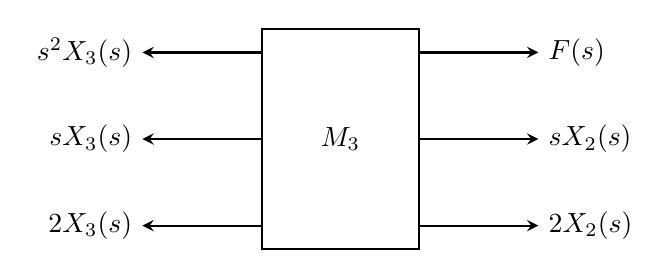
\begin{tikzpicture}[
    force/.style={->,>=stealth,thick}
]
    \node[draw, thick, minimum width=2cm, minimum height=2.8cm, label=center:$M_3$] (m3) {};

    \draw[force] ([yshift=1.1cm]m3.west) -- ++(-1.5,0) node[left] {$s^2X_3(s)$};
    \draw[force] ([yshift=0cm]m3.west) -- ++(-1.5,0) node[left] {$sX_3(s)$};
    \draw[force] ([yshift=-1.1cm]m3.west) -- ++(-1.5,0) node[left] {$2X_3(s)$};
    
    \draw[force] ([yshift=1.1cm]m3.east) -- ++(1.5,0) node[right] {$F(s)$};
    \draw[force] ([yshift=0cm]m3.east) -- ++(1.5,0) node[right] {$sX_2(s)$};
    \draw[force] ([yshift=-1.1cm]m3.east) -- ++(1.5,0) node[right] {$2X_2(s)$};
\end{tikzpicture}
\end{figure}

The resulting equation in the Laplace domain is:
\begin{equation}
-(s + 2)X_2(s) + (s^2 + s + 2)X_3(s) = F(s) \tag{3}
\end{equation}

\noindent\textbf{Solving the System using Cramer's Rule}
\vspace{12pt}

The system can be expressed in matrix form $A\mathbf{x} = \mathbf{b}$:
$$
\begin{bmatrix}
s^2 + 3s + 3 & -(2s + 1) & 0 \\
-(2s + 1) & s^2 + 3s + 3 & -(s + 2) \\
0 & -(s + 2) & s^2 + s + 2
\end{bmatrix}
\begin{bmatrix}
X_1(s) \\
X_2(s) \\
X_3(s)
\end{bmatrix}
=
\begin{bmatrix}
0 \\
0 \\
F(s)
\end{bmatrix}
$$

The solution for $X_1(s)$ is $G(s) = \frac{X_1(s)}{F(s)} = \frac{\det(A_1)}{\det(A)} = \frac{\Delta_1}{\Delta}$.

\vspace{12pt}
\noindent\textbf{Calculating the Numerator Determinant, $\Delta_1$}:
$$ \Delta_1 = \det
\begin{bmatrix}
0 & -(2s + 1) & 0 \\
0 & s^2 + 3s + 3 & -(s + 2) \\
F(s) & -(s + 2) & s^2 + s + 2
\end{bmatrix}
= (2s^2 + 5s + 2)F(s) $$

{Calculating the Denominator Determinant, $\Delta$}:
$$\Delta = \det(A) = s^6 + 7s^5 + 18s^4 + 30s^3 + 25s^2 + 12s + 4$$

{Constructing the Transfer Function}
$$G(s) = \frac{X_1(s)}{F(s)} = \frac{\Delta_1}{\Delta F(s)}$$

Expanding the denominator yields the simplified standard form:
\[
\boxed{
G(s) = \frac{2s^2 + 5s + 2}{s^6 + 7s^5 + 18s^4 + 30s^3 + 25s^2 + 12s + 4}
}
\]

% Problem 13 - Translational Mechanical Transfer Function

\newpage
  \setcounter{page}{20}  
\noindent\rule{\textwidth}{1pt}
\noindent\textbf{Problem 13} \hfill
\\For the translational mechanical system diagram shown below, determine the transfer function $G(s)=X_1(s)/F(s)$.
% P6 Figure
% #1
% #9.1
\begin{center}
\resizebox{\textwidth}{!}{%
    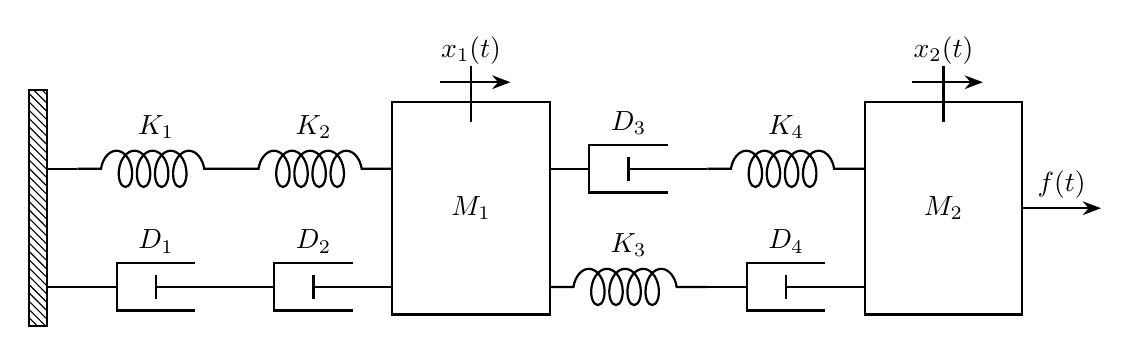
\begin{tikzpicture}[point/.style={coordinate}, >={Stealth}, thick]
        \node[wall] (W) at (-0.5,1) {};

        %damper
        \hdamper{(0,0)}{$D_1 $}
        \hdamper{(2,0)}{$D_2 $}
        \hdamper{(6,1.5)}{$D_3 $}
        \hdamper{(8,0)}{$D_4 $}

        %spring
        \hspring{0,1.5}{$K_1 $ }
        \hspring{2,1.5}{$K_2 $ }
        \hspring{6,0}{$K_3 $ }
        \hspring{8,1.5}{$K_4 $ }
        
        %mass
        \tbody{5,1}{$M_1$}{$x_1(t)$}{M1};
        \tbody{11,1}{$M_2$}{$x_2(t)$}{M2};

    % f(t)
        \node at (12.5,1.3) { $f(t)$};
        \draw[->] (12,1) -- (13,1);

        % \node at (x+.5,1.3) { $f(t)$};
        % \draw[->] (x,1) -- (x+1,1);
        
        \draw (-0.38,0) -- (0,0);
        \draw (-0.38,1.5) -- (0,1.5);
        
    \end{tikzpicture}
}
\end{center}
\noindent\rule{\textwidth}{1pt}

\vspace{12pt}

\noindent\textbf{\textit{Given:}}
\[
\begin{aligned}
M_1 &= 1\, \text{kg} & K_1 &= 1\, \text{N/m} & D_1 &= 1\, \text{N}\cdot\text{s/m} \\
M_2 &= 1\, \text{kg} & K_2 &= 1\, \text{N/m} & D_2 &= 1\, \text{N}\cdot\text{s/m} \\
& & K_3 &= 1\, \text{N/m} & D_3 &= 1\, \text{N}\cdot\text{s/m} \\
& & K_4 &= 1\, \text{N/m} & D_4 &= 1\, \text{N}\cdot\text{s/m}
\end{aligned}
\]

\vspace{12pt}

\noindent \textbf{\textit{Required:}}
\[
G(s) = \frac{X_1(s)}{F(s)}
\]

\vspace{12pt}

\noindent \textbf{\textit{Solution:}}

\vspace{12pt}

\noindent \textbf{Deriving the Equations of Motion}
\vspace{12pt}

\noindent We apply Newton's second law ($\sum F = ma$) to each mass, with the positive direction of motion to the right. 

\vspace{12pt}
{For Mass $M_1$:}
\begin{figure}[h!]
\centering
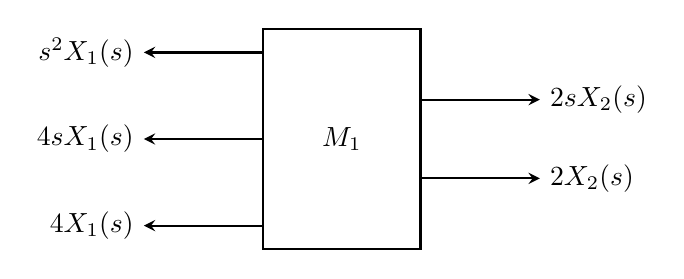
\begin{tikzpicture}[
    force/.style={->,>=stealth,thick}
]
    \node[draw, thick, minimum width=2cm, minimum height=2.8cm, label=center:$M_1$] (m1) {};

    \draw[force] ([yshift=1.1cm]m1.west) -- ++(-1.5,0) node[left] {$s^2X_1(s)$};
    \draw[force] ([yshift=0cm]m1.west) -- ++(-1.5,0) node[left] {$4sX_1(s)$};
    \draw[force] ([yshift=-1.1cm]m1.west) -- ++(-1.5,0) node[left] {$4X_1(s)$};

    \draw[force] ([yshift=0.5cm]m1.east) -- ++(1.5,0) node[right] {$2sX_2(s)$};
    \draw[force] ([yshift=-0.5cm]m1.east) -- ++(1.5,0) node[right] {$2X_2(s)$};
\end{tikzpicture}
\end{figure}

The resulting equation in the Laplace domain is:
\begin{equation}
(s^2 + 4s + 4)X_1(s) - (2s + 2)X_2(s) = 0 \tag{1}
\end{equation}

\vspace{12pt}
{For Mass $M_2$:}
\begin{figure}[h!]
\centering
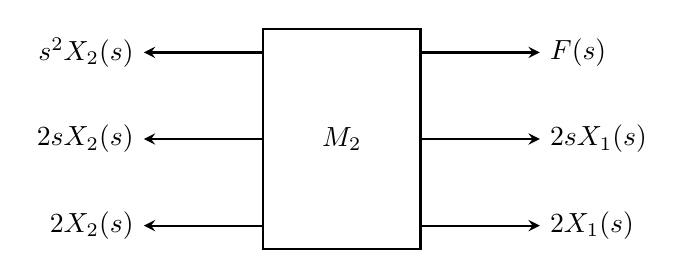
\begin{tikzpicture}[
    force/.style={->,>=stealth,thick}
]
    \node[draw, thick, minimum width=2cm, minimum height=2.8cm, label=center:$M_2$] (m2) {};

    \draw[force] ([yshift=1.1cm]m2.west) -- ++(-1.5,0) node[left] {$s^2X_2(s)$};
    \draw[force] ([yshift=0cm]m2.west) -- ++(-1.5,0) node[left] {$2sX_2(s)$};
    \draw[force] ([yshift=-1.1cm]m2.west) -- ++(-1.5,0) node[left] {$2X_2(s)$};
    
    \draw[force] ([yshift=1.1cm]m2.east) -- ++(1.5,0) node[right] {$F(s)$};
    \draw[force] ([yshift=0cm]m2.east) -- ++(1.5,0) node[right] {$2sX_1(s)$};
    \draw[force] ([yshift=-1.1cm]m2.east) -- ++(1.5,0) node[right] {$2X_1(s)$};
\end{tikzpicture}
\end{figure}

The resulting equation in the Laplace domain is:
\begin{equation}
-(2s + 2)X_1(s) + (s^2 + 2s + 2)X_2(s) = F(s) \tag{2}
\end{equation}

\newpage
\noindent\textbf{Solving the System using Cramer's Rule}
\vspace{12pt}

The system can be expressed in matrix form $A\mathbf{x} = \mathbf{b}$:
$$
\begin{bmatrix}
s^2 + 4s + 4 & -(2s + 2) \\
-(2s + 2) & s^2 + 2s + 2
\end{bmatrix}
\begin{bmatrix}
X_1(s) \\
X_2(s)
\end{bmatrix}
=
\begin{bmatrix}
0 \\
F(s)
\end{bmatrix}
$$

The solution for $X_1(s)$ is $G(s) = \frac{X_1(s)}{F(s)} = \frac{\det(A_1)}{\det(A)} = \frac{\Delta_1}{\Delta}$.

\vspace{12pt}
\noindent\textbf{Calculating the Numerator Determinant, $\Delta_1$}:
$$ \Delta_1 = \det
\begin{bmatrix}
0 & -(2s + 2) \\
F(s) & s^2 + 2s + 2
\end{bmatrix}
= (2s + 2)F(s) $$

{Calculating the Denominator Determinant, $\Delta$}:
$$\Delta = \det(A) = s^4 + 6s^3 + 10s^2 + 8s + 4$$

{Constructing the Transfer Function}
$$G(s) = \frac{X_1(s)}{F(s)} = \frac{\Delta_1}{\Delta F(s)}$$

Expanding the denominator yields the simplified standard form:
\[
\boxed{
G(s) = \frac{2s + 2}{s^4 + 6s^3 + 10s^2 + 8s + 4}
}
\]

% Problem 14 - Translational Mechanical Transfer Function

\newpage
  \setcounter{page}{22}  
\noindent\rule{\textwidth}{1pt}
\noindent\textbf{Problem 14} \hfill
\\For the translational mechanical system diagram shown below, determine the transfer function $G(s)=X_1(s)/F(s)$.
% P6 Figure
% #1
% #9
\begin{center}
\resizebox{\textwidth}{!}{%
    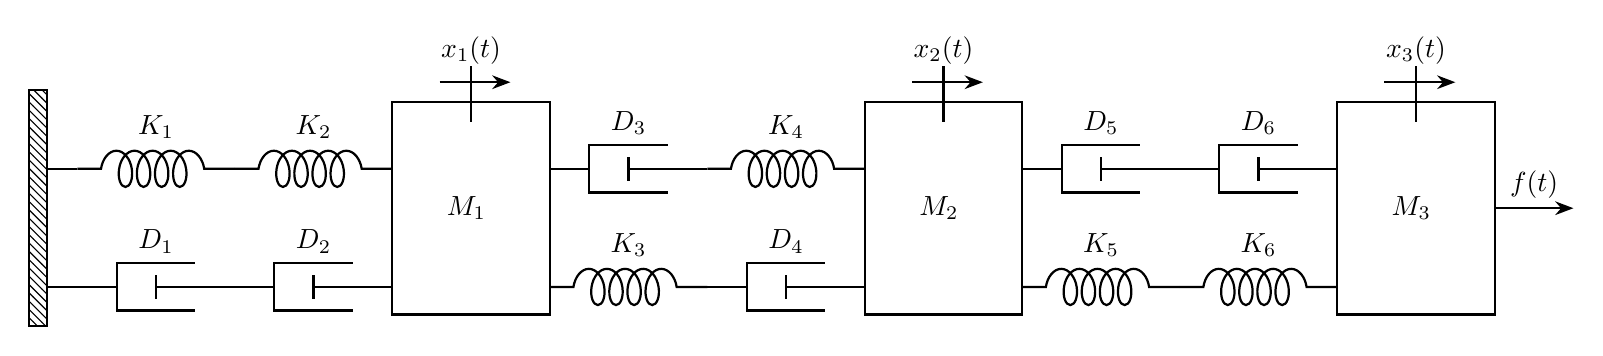
\begin{tikzpicture}[point/.style={coordinate}, >={Stealth}, thick]
        \node[wall] (W) at (-0.5,1) {};

        %damper
        \hdamper{(0,0)}{$D_1 $}
        \hdamper{(2,0)}{$D_2 $}
        \hdamper{(6,1.5)}{$D_3 $}
        \hdamper{(8,0)}{$D_4 $}
        \hdamper{(12,1.5)}{$D_5 $}
        \hdamper{(14,1.5)}{$D_6 $}

        %spring
        \hspring{0,1.5}{$K_1 $}
        \hspring{2,1.5}{$K_2 $}
        \hspring{6,0}{$K_3 $}
        \hspring{8,1.5}{$K_4 $}
        \hspring{12,0}{$K_5 $}
        \hspring{14,0}{$K_6 $}
        
        %mass
        \tbody{5,1}{$M_1$ }{$x_1(t)$}{M1};
        \tbody{11,1}{$M_2$ }{$x_2(t)$}{M2};
        \tbody{17,1}{$M_3$ }{$x_3(t)$}{M3};

    % f(t)
        \node at (18.5,1.3) { $f(t)$};
        \draw[->] (18,1) -- (19,1);

        % \node at (x+.5,1.3) { $f(t)$};
        % \draw[->] (x,1) -- (x+1,1);
        
        \draw (-0.38,0) -- (0,0);
        \draw (-0.38,1.5) -- (0,1.5);
        
    \end{tikzpicture}
}
\end{center}
\noindent\rule{\textwidth}{1pt}

\vspace{12pt}

\noindent\textbf{\textit{Given:}}
\[
\begin{aligned}
M_1 &= 1\, \text{kg} & K_1 &= 1\, \text{N/m} & D_1 &= 1\, \text{N}\cdot\text{s/m} \\
M_2 &= 1\, \text{kg} & K_2 &= 1\, \text{N/m} & D_2 &= 1\, \text{N}\cdot\text{s/m} \\
M_3 &= 1\, \text{kg} & K_3 &= 1\, \text{N/m} & D_3 &= 1\, \text{N}\cdot\text{s/m} \\
& & K_4 &= 1\, \text{N/m} & D_4 &= 1\, \text{N}\cdot\text{s/m} \\
& & K_5 &= 1\, \text{N/m} & D_5 &= 1\, \text{N}\cdot\text{s/m} \\
& & K_6 &= 1\, \text{N/m} & D_6 &= 1\, \text{N}\cdot\text{s/m}
\end{aligned}
\]

\vspace{12pt}

\noindent \textbf{\textit{Required:}}
\[
G(s) = \frac{X_1(s)}{F(s)}
\]

\vspace{12pt}

\noindent \textbf{\textit{Solution:}}

\vspace{12pt}

\noindent \textbf{Deriving the Equations of Motion}
\vspace{12pt}

\noindent We apply Newton's second law ($\sum F = ma$) to each mass, with the positive direction of motion to the right. 

\vspace{12pt}
{For Mass $M_1$:}
\begin{figure}[h!]
\centering
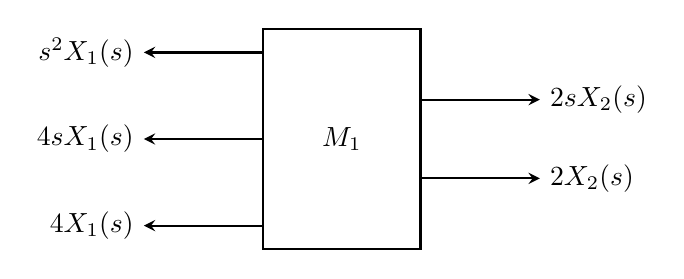
\begin{tikzpicture}[
    force/.style={->,>=stealth,thick}
]
    \node[draw, thick, minimum width=2cm, minimum height=2.8cm, label=center:$M_1$] (m1) {};

    \draw[force] ([yshift=1.1cm]m1.west) -- ++(-1.5,0) node[left] {$s^2X_1(s)$};
    \draw[force] ([yshift=0cm]m1.west) -- ++(-1.5,0) node[left] {$4sX_1(s)$};
    \draw[force] ([yshift=-1.1cm]m1.west) -- ++(-1.5,0) node[left] {$4X_1(s)$};

    \draw[force] ([yshift=0.5cm]m1.east) -- ++(1.5,0) node[right] {$2sX_2(s)$};
    \draw[force] ([yshift=-0.5cm]m1.east) -- ++(1.5,0) node[right] {$2X_2(s)$};
\end{tikzpicture}
\end{figure}

The resulting equation in the Laplace domain is:
\begin{equation}
(s^2 + 4s + 4)X_1(s) - (2s + 2)X_2(s) = 0 \tag{1}
\end{equation}

\vspace{12pt}
{For Mass $M_2$:}
\begin{figure}[h!]
\centering
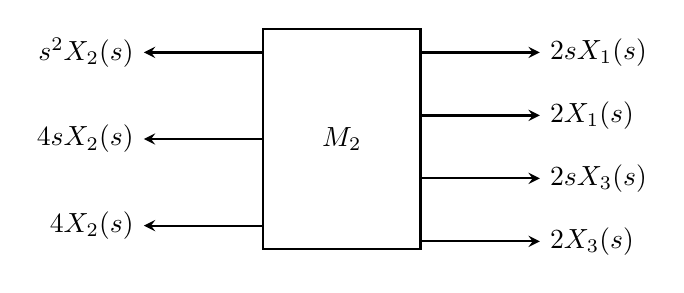
\begin{tikzpicture}[
    force/.style={->,>=stealth,thick}
]
    \node[draw, thick, minimum width=2cm, minimum height=2.8cm, label=center:$M_2$] (m2) {};

    \draw[force] ([yshift=1.1cm]m2.west) -- ++(-1.5,0) node[left] {$s^2X_2(s)$};
    \draw[force] ([yshift=0cm]m2.west) -- ++(-1.5,0) node[left] {$4sX_2(s)$};
    \draw[force] ([yshift=-1.1cm]m2.west) -- ++(-1.5,0) node[left] {$4X_2(s)$};
    
    \draw[force] ([yshift=1.1cm]m2.east) -- ++(1.5,0) node[right] {$2sX_1(s)$};
    \draw[force] ([yshift=0.3cm]m2.east) -- ++(1.5,0) node[right] {$2X_1(s)$};
    \draw[force] ([yshift=-0.5cm]m2.east) -- ++(1.5,0) node[right] {$2sX_3(s)$};
    \draw[force] ([yshift=-1.3cm]m2.east) -- ++(1.5,0) node[right] {$2X_3(s)$};
\end{tikzpicture}
\end{figure}

The resulting equation in the Laplace domain is:
\begin{equation}
-(2s + 2)X_1(s) + (s^2 + 4s + 4)X_2(s) - (2s + 2)X_3(s) = 0 \tag{2}
\end{equation}

\newpage

\vspace{12pt}
{For Mass $M_3$:}
\begin{figure}[h!]
\centering
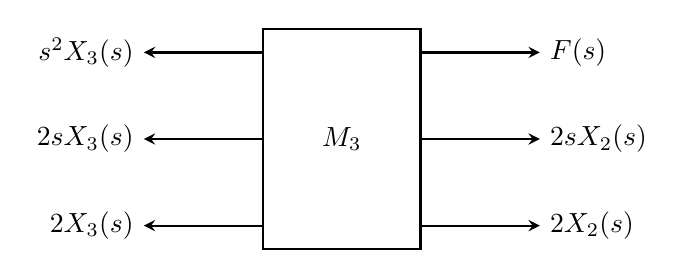
\begin{tikzpicture}[
    force/.style={->,>=stealth,thick}
]
    \node[draw, thick, minimum width=2cm, minimum height=2.8cm, label=center:$M_3$] (m3) {};

    \draw[force] ([yshift=1.1cm]m3.west) -- ++(-1.5,0) node[left] {$s^2X_3(s)$};
    \draw[force] ([yshift=0cm]m3.west) -- ++(-1.5,0) node[left] {$2sX_3(s)$};
    \draw[force] ([yshift=-1.1cm]m3.west) -- ++(-1.5,0) node[left] {$2X_3(s)$};
    
    \draw[force] ([yshift=1.1cm]m3.east) -- ++(1.5,0) node[right] {$F(s)$};
    \draw[force] ([yshift=0cm]m3.east) -- ++(1.5,0) node[right] {$2sX_2(s)$};
    \draw[force] ([yshift=-1.1cm]m3.east) -- ++(1.5,0) node[right] {$2X_2(s)$};
\end{tikzpicture}
\end{figure}

The resulting equation in the Laplace domain is:
\begin{equation}
-(2s + 2)X_2(s) + (s^2 + 2s + 2)X_3(s) = F(s) \tag{3}
\end{equation}

\noindent\textbf{Solving the System using Cramer's Rule}
\vspace{12pt}

The system can be expressed in matrix form $A\mathbf{x} = \mathbf{b}$:
$$
\begin{bmatrix}
s^2 + 4s + 4 & -(2s + 2) & 0 \\
-(2s + 2) & s^2 + 4s + 4 & -(2s + 2) \\
0 & -(2s + 2) & s^2 + 2s + 2
\end{bmatrix}
\begin{bmatrix}
X_1(s) \\
X_2(s) \\
X_3(s)
\end{bmatrix}
=
\begin{bmatrix}
0 \\
0 \\
F(s)
\end{bmatrix}
$$

The solution for $X_1(s)$ is $G(s) = \frac{X_1(s)}{F(s)} = \frac{\det(A_1)}{\det(A)} = \frac{\Delta_1}{\Delta}$.

\vspace{12pt}
\noindent\textbf{Calculating the Numerator Determinant, $\Delta_1$}:
$$ \Delta_1 = \det
\begin{bmatrix}
0 & -(2s + 2) & 0 \\
0 & s^2 + 4s + 4 & -(2s + 2) \\
F(s) & -(2s + 2) & s^2 + 2s + 2
\end{bmatrix}
= (2s + 2)^2F(s) $$

{Calculating the Denominator Determinant, $\Delta$}:
$$\Delta = \det(A) = s^6 + 10s^5 + 37s^4 + 64s^3 + 54s^2 + 20s + 4$$

{Constructing the Transfer Function}
$$G(s) = \frac{X_1(s)}{F(s)} = \frac{\Delta_1}{\Delta F(s)}$$

Expanding the denominator yields the simplified standard form:
\[
\boxed{
G(s) = \frac{(2s + 2)^2}{s^6 + 10s^5 + 37s^4 + 64s^3 + 54s^2 + 20s + 4}
}
\]

% Problem 15 - Translational Mechanical Transfer Function

\newpage
  \setcounter{page}{24}  
\noindent\rule{\textwidth}{1pt}
\noindent\textbf{Problem 15} \hfill
\\For the translational mechanical system diagram shown below, determine the transfer function $G(s)=X_1(s)/F(s)$.
% P15 Figure
\begin{center}
    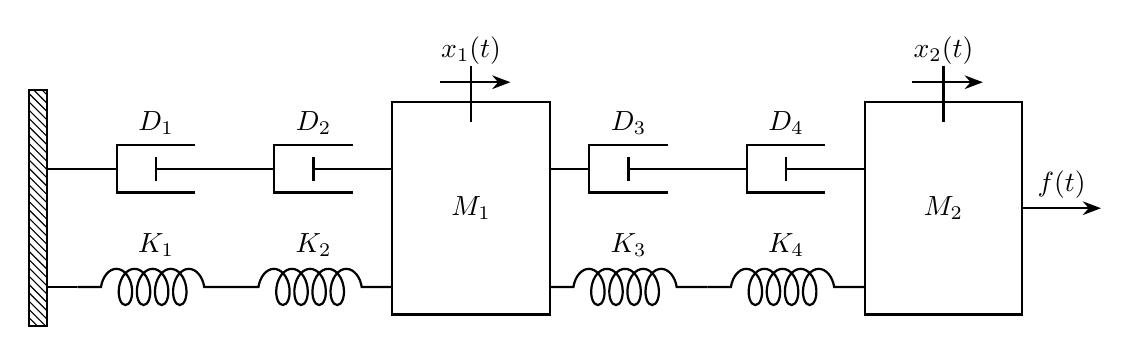
\begin{tikzpicture}[point/.style={coordinate}, >={Stealth}, thick]
        \node[wall] (W) at (-0.5,1) {};

        % 2ND LAYER
        % 0 - 2
        \hdamper{(0,1.5)}{$D_1 $}
        % 2 - 4
        \hdamper{(2,1.5)}{$D_2 $}
        % 6 - 8
        \hdamper{(6,1.5)}{$D_3 $}
        % 8 - 10
        \hdamper{(8,1.5)}{$D_4 $}

        % 1ST LAYER
        % 0 - 2
        \hspring{0,0}{$K_1 $}
        % 2 - 4
        \hspring{2,0}{$K_2 $}
        % 6 - 8
        \hspring{6,0}{$K_3 $}
        % 8 - 10
        \hspring{8,0}{$K_4 $}

        % 5 - 6
        \tbody{5,1}{$M_1$}{$x_1(t)$}{M1};
        % 11 - 12
        \tbody{11,1}{$M_2$}{$x_2(t)$}{M2};

    % f(t)
        \node at (12.5,1.3) { $f(t)$};
        \draw[->] (12,1) -- (13,1);

        % \node at (x+.5,1.3) { $f(t)$};
        % \draw[->] (x,1) -- (x+1,1);
        
        \draw (-0.38,0) -- (0,0);
        \draw (-0.38,1.5) -- (0,1.5);
    \end{tikzpicture}
\end{center}
\noindent\rule{\textwidth}{1pt}

\vspace{12pt}

\noindent\textbf{\textit{Given:}}
\[
\begin{aligned}
M_1 &= 2\, \text{kg} & K_1 &= 3\, \text{N/m} & D_1 &= 1\, \text{N}\cdot\text{s/m} \\
M_2 &= 3\, \text{kg} & K_2 &= 2\, \text{N/m} & D_2 &= 2\, \text{N}\cdot\text{s/m} \\
& & K_3 &= 1\, \text{N/m} & D_3 &= 1\, \text{N}\cdot\text{s/m} \\
& & K_4 &= 2\, \text{N/m} & D_4 &= 2\, \text{N}\cdot\text{s/m}
\end{aligned}
\]

\vspace{12pt}

\noindent \textbf{\textit{Required:}}
\[
G(s) = \frac{X_1(s)}{F(s)}
\]

\vspace{12pt}

\noindent \textbf{\textit{Solution:}}

\vspace{12pt}

\noindent \textbf{Deriving the Equations of Motion}
\vspace{12pt}

\noindent We apply Newton's second law ($\sum F = ma$) to each mass, with the positive direction of motion to the right. 

\vspace{12pt}
{For Mass $M_1$:}
\begin{figure}[h!]
\centering
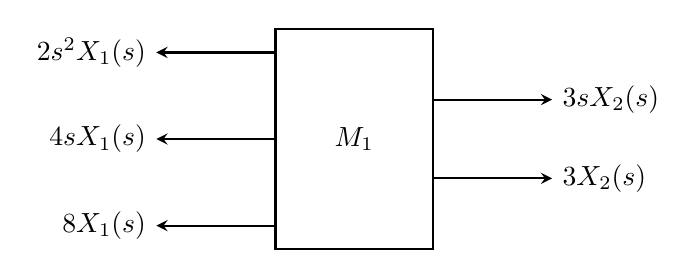
\begin{tikzpicture}[
    force/.style={->,>=stealth,thick}
]
    \node[draw, thick, minimum width=2cm, minimum height=2.8cm, label=center:$M_1$] (m1) {};

    \draw[force] ([yshift=1.1cm]m1.west) -- ++(-1.5,0) node[left] {$2s^2X_1(s)$};
    \draw[force] ([yshift=0cm]m1.west) -- ++(-1.5,0) node[left] {$4sX_1(s)$};
    \draw[force] ([yshift=-1.1cm]m1.west) -- ++(-1.5,0) node[left] {$8X_1(s)$};

    \draw[force] ([yshift=0.5cm]m1.east) -- ++(1.5,0) node[right] {$3sX_2(s)$};
    \draw[force] ([yshift=-0.5cm]m1.east) -- ++(1.5,0) node[right] {$3X_2(s)$};
\end{tikzpicture}
\end{figure}

The resulting equation in the Laplace domain is:
\begin{equation}
(2s^2 + 4s + 8)X_1(s) - (3s + 3)X_2(s) = 0 \tag{1}
\end{equation}

\vspace{12pt}
{For Mass $M_2$:}
\begin{figure}[h!]
\centering
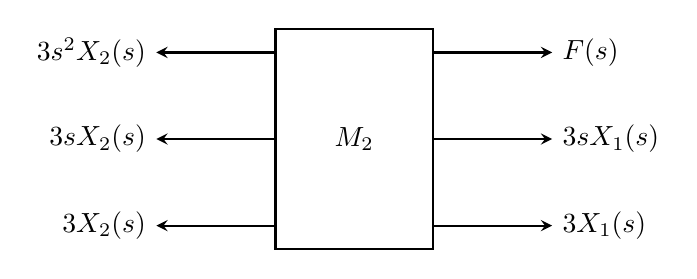
\begin{tikzpicture}[
    force/.style={->,>=stealth,thick}
]
    \node[draw, thick, minimum width=2cm, minimum height=2.8cm, label=center:$M_2$] (m2) {};

    \draw[force] ([yshift=1.1cm]m2.west) -- ++(-1.5,0) node[left] {$3s^2X_2(s)$};
    \draw[force] ([yshift=0cm]m2.west) -- ++(-1.5,0) node[left] {$3sX_2(s)$};
    \draw[force] ([yshift=-1.1cm]m2.west) -- ++(-1.5,0) node[left] {$3X_2(s)$};
    
    \draw[force] ([yshift=1.1cm]m2.east) -- ++(1.5,0) node[right] {$F(s)$};
    \draw[force] ([yshift=0cm]m2.east) -- ++(1.5,0) node[right] {$3sX_1(s)$};
    \draw[force] ([yshift=-1.1cm]m2.east) -- ++(1.5,0) node[right] {$3X_1(s)$};
\end{tikzpicture}
\end{figure}

The resulting equation in the Laplace domain is:
\begin{equation}
-(3s + 3)X_1(s) + (3s^2 + 3s + 3)X_2(s) = F(s) \tag{2}
\end{equation}

\newpage
\noindent\textbf{Solving the System using Cramer's Rule}
\vspace{12pt}

The system can be expressed in matrix form $A\mathbf{x} = \mathbf{b}$:
$$
\begin{bmatrix}
2s^2 + 4s + 8 & -(3s + 3) \\
-(3s + 3) & 3s^2 + 3s + 3
\end{bmatrix}
\begin{bmatrix}
X_1(s) \\
X_2(s)
\end{bmatrix}
=
\begin{bmatrix}
0 \\
F(s)
\end{bmatrix}
$$

The solution for $X_1(s)$ is $G(s) = \frac{X_1(s)}{F(s)} = \frac{\det(A_1)}{\det(A)} = \frac{\Delta_1}{\Delta}$.

\vspace{12pt}
\noindent\textbf{Calculating the Numerator Determinant, $\Delta_1$}:
$$ \Delta_1 = \det
\begin{bmatrix}
0 & -(3s + 3) \\
F(s) & 3s^2 + 3s + 3
\end{bmatrix}
= (3s + 3)F(s) $$

{Calculating the Denominator Determinant, $\Delta$}:
$$\Delta = \det(A) = 6s^4 + 18s^3 + 33s^2 + 18s + 15$$

{Constructing the Transfer Function}
$$G(s) = \frac{X_1(s)}{F(s)} = \frac{\Delta_1}{\Delta F(s)}$$

Expanding the denominator yields the simplified standard form:
\[
\boxed{
G(s) = \frac{3s + 3}{6s^4 + 18s^3 + 33s^2 + 18s + 15}
}
\]

% Problem 16 - Rotational Mechanical System

\newpage
  \setcounter{page}{25}  
\noindent\rule{\textwidth}{1pt}
\noindent\textbf{Problem 16} \hfill
\\For the rotational mechanical system shown in the diagram below, determine the transfer function $G(s)=\theta_3(s)/T(s)$.
% P16 Figure
\begin{center}
\resizebox{\textwidth}{!}{%
    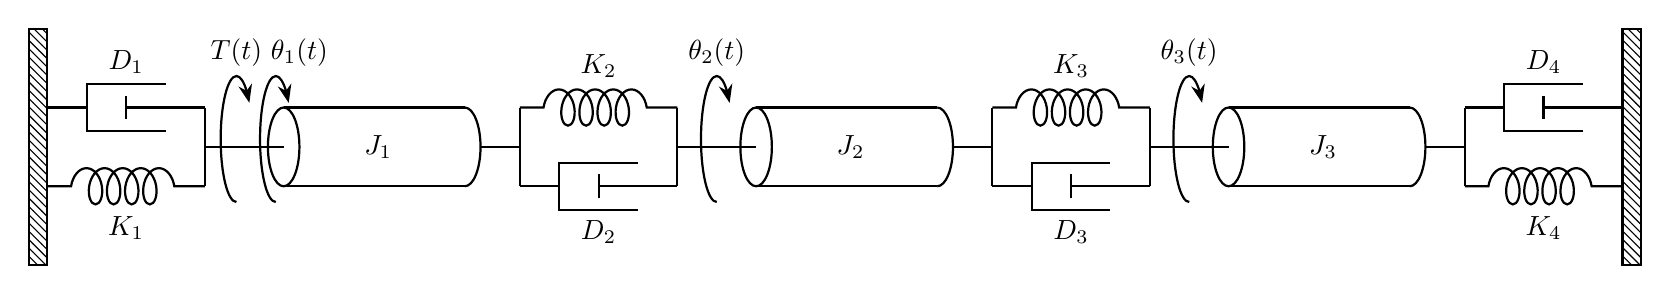
\begin{tikzpicture}[point/.style={coordinate}, >={Stealth}, thick]
        % Left Wall
        \node[wall] (W) at (-0.12,0) {};

        \hdamper{(0,0.5)}{$D_1$}
        \blspring{0,-0.5}{$K_1$}

        \draw (2,0.5) -- (2,-0.5);

        \frbody{(2,0)}

        \draw (6,0.5) -- (6,-0.5);

        \hspring{6,0.5}{$K_2$}
        \bldamper{(6,-0.5)}{$D_2$}

        \draw (8,0.5) -- (8,-0.5); 

        \rbody{(8,0)}{$J_2$}{$\theta_2(t)$}
        
        \draw (12,0.5) -- (12,-0.5);

        \hspring{12,0.5}{$K_3$}
        \bldamper{(12,-0.5)}{$D_3$}

        \draw (14,0.5) -- (14,-0.5); 

        \rbody{(14,0)}{$J_3$}{$\theta_3(t)$}

        \draw (18,0.5) -- (18,-0.5); 

        \hdamper{(18,0.5)}{$D_4$}
        \blspring{18,-0.5}{$K_4$}

        \rwall{20,0}
    \end{tikzpicture}
}
\end{center}
\noindent\rule{\textwidth}{1pt}

\vspace{12pt}   
\noindent\textbf{\textit{Given:}}
\[
\begin{aligned}
J_1 &= 2\, \text{kg}\cdot\text{m}^2 & K_1 &= 4\, \text{N}\cdot\text{m/rad} & D_1 &= 6\, \text{N}\cdot\text{m}\cdot\text{s/rad} \\
J_2 &= 1\, \text{kg}\cdot\text{m}^2 & K_2 &= 3\, \text{N}\cdot\text{m/rad} & D_2 &= 2\, \text{N}\cdot\text{m}\cdot\text{s/rad} \\
J_3 &= 1\, \text{kg}\cdot\text{m}^2 & K_3 &= 2\, \text{N}\cdot\text{m/rad} & D_3 &= 1\, \text{N}\cdot\text{m}\cdot\text{s/rad} \\
& & K_4 &= 1\, \text{N}\cdot\text{m/rad} & D_4 &= 4\, \text{N}\cdot\text{m}\cdot\text{s/rad}
\end{aligned}
\]

\vspace{12pt}

\noindent \textbf{\textit{Required:}}
\[
G(s) = \frac{\theta_3(s)}{T(s)}
\]

\vspace{12pt}

\noindent \textbf{\textit{Solution:}}\\

% Start of Solution
\begin{enumerate}[label=(\alph*), itemindent=*, leftmargin=*, nolistsep]
    
    \item Draw the Free Body Diagrams of the provided masses
\vspace{10pt}
    \begin{center}
            \textbf{Free Body Diagram at $J_1$} \\[6pt]
            \vspace{15pt}
            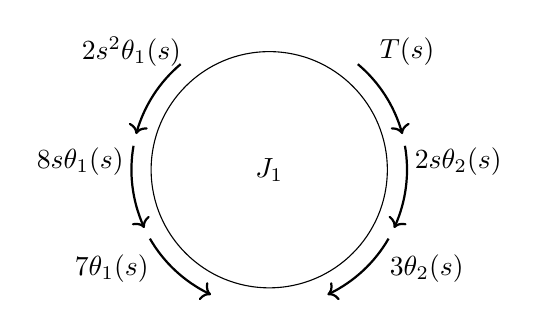
\begin{tikzpicture}
                % Circle
                \draw (0,0) circle (1.5);
                \node at (0,0) {$J_1$};
                % Left-hand Arrows
                \draw[->, thick] (0,0) ++(130:1.75) arc[start angle=130, end angle=165, radius=1.75];
                \node at (-1.75,1.5){$2s^2\theta_1(s)$};
                \draw[->, thick] (0,0) ++(170:1.75) arc[start angle=170, end angle=205, radius=1.75];
                \node at (-2.4,0.1){$8s\theta_1(s)$};
                \draw[->, thick] (0,0) ++(210:1.75) arc[start angle=210, end angle=245, radius=1.75];
                \node at (-2,-1.25){$7\theta_1(s)$};
                % Right-hand Arrows
                \draw[->, thick] (0,0) ++(50:1.75) arc[start angle=50, end angle=15, radius=1.75];
                \node at (1.75,1.5){$T(s)$};
                \draw[->, thick] (0,0) ++(10:1.75) arc[start angle=10, end angle=-25, radius=1.75];
                \node at (2.4,0.1){$2s\theta_2(s)$};
                \draw[->, thick] (0,0) ++(-30:1.75) arc[start angle=-30, end angle=-65, radius=1.75];
                \node at (2,-1.25){$3\theta_2(s)$};
            \end{tikzpicture}
    
            % Equations under J1
            \vspace{15pt}
    
            $\sum T_0 = 0 \quad\text{(clockwise, +)}$ \\ \vspace{10pt}
            $T(s) - (2s^2 + 8s + 7)\theta_1(s) + (2s + 3)\theta_2(s) = 0$ \\ \vspace{10pt}
            $T(s) = (2s^2 + 8s + 7)\theta_1(s) - (2s + 3)\theta_2(s)$

    \end{center}

\vspace{15pt}
    \begin{center}
        %---------------- RIGHT SIDE: J2 ----------------%
            \textbf{Free Body Diagram at $J_2$} \\[6pt]
            \vspace{15pt}
            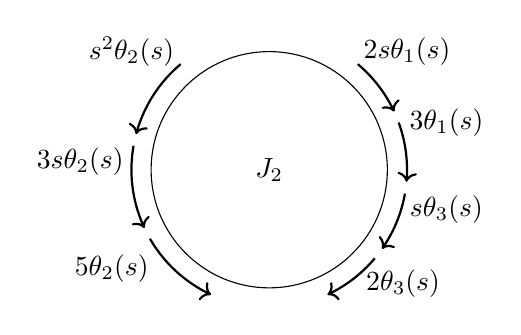
\begin{tikzpicture}
                % Circle
                \draw (0,0) circle (1.5);
                \node at (0,0) {$J_2$};
                % Left-hand Arrows
                \draw[->, thick] (0,0) ++(130:1.75) arc[start angle=130, end angle=165, radius=1.75];
                \node at (-1.75,1.5){$s^2\theta_2(s)$};
                \draw[->, thick] (0,0) ++(170:1.75) arc[start angle=170, end angle=205, radius=1.75];
                \node at (-2.4,0.1){$3s\theta_2(s)$};
                \draw[->, thick] (0,0) ++(210:1.75) arc[start angle=210, end angle=245, radius=1.75];
                \node at (-2,-1.25){$5\theta_2(s)$};
                % Right-hand Arrows
                \draw[->, thick] (0,0) ++(50:1.75) arc[start angle=50, end angle=25, radius=1.75];
                \node at (1.75,1.5){$2s\theta_1(s)$};
                \draw[->, thick] (0,0) ++(20:1.75) arc[start angle=20, end angle=-5, radius=1.75];
                \node at (2.25,0.6){$3\theta_1(s)$};
                \draw[->, thick] (0,0) ++(-10:1.75) arc[start angle=-10, end angle=-35, radius=1.75];
                \node at (2.25,-0.5){$s\theta_3(s)$};
                \draw[->, thick] (0,0) ++(-40:1.75) arc[start angle=-40, end angle=-65, radius=1.75];
                \node at (1.7,-1.45){$2\theta_3(s)$};
            \end{tikzpicture}
    
            % Equations under J2
    
    \vspace{15pt}
    

        $\sum T_0 = 0 \quad\text{(clockwise, +)}$ \\ \vspace{10pt}
        $0 = (2s + 3)\theta_1(s) - (s^2 + 3s + 5)\theta_2(s) + (s + 2)\theta_3(s)$\\ \vspace{10pt}
        $0 = -(2s + 3)\theta_1(s) + (s^2 + 3s + 5)\theta_2(s) - (s + 2)\theta_3(s)$

    \end{center}

    \vspace{15pt}
    \begin{center}
            \textbf{Free Body Diagram at $J_3$} \\[6pt]
            \vspace{15pt}
            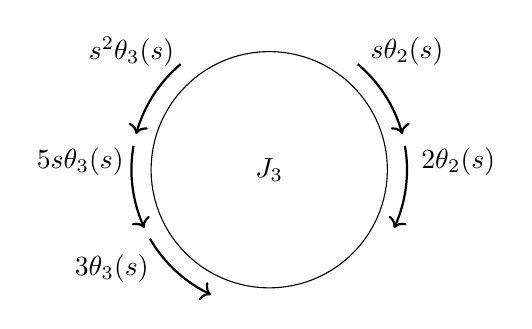
\begin{tikzpicture}
                % Circle
                \draw (0,0) circle (1.5);
                \node at (0,0) {$J_3$};
                % Left-hand Arrows
                \draw[->, thick] (0,0) ++(130:1.75) arc[start angle=130, end angle=165, radius=1.75];
                \node at (-1.75,1.5){$s^2\theta_3(s)$};
                \draw[->, thick] (0,0) ++(170:1.75) arc[start angle=170, end angle=205, radius=1.75];
                \node at (-2.4,0.1){$5s\theta_3(s)$};
                \draw[->, thick] (0,0) ++(210:1.75) arc[start angle=210, end angle=245, radius=1.75];
                \node at (-2,-1.25){$3\theta_3(s)$};
                % Right-hand Arrows
                \draw[->, thick] (0,0) ++(50:1.75) arc[start angle=50, end angle=15, radius=1.75];
                \node at (1.75,1.5){$s\theta_2(s)$};
                \draw[->, thick] (0,0) ++(10:1.75) arc[start angle=10, end angle=-25, radius=1.75];
                \node at (2.4,0.1){$2\theta_2(s)$};
            \end{tikzpicture}
    
            % Equations under J3
            \vspace{15pt}
    
            $\sum T_0 = 0 \quad\text{(clockwise, +)}$ \\ \vspace{10pt}
            $0 = (s + 2)\theta_2(s) - (s^2 + 5s + 3)\theta_3(s)$ \\ \vspace{10pt}
            $0 = -(s + 2)\theta_2(s) + (s^2 + 5s + 3)\theta_3(s)$ 

    \end{center}
\vspace{15pt}
    \item Write the displacement equations and provide the matrix form
\begin{center}
    T(s) $= (2s^2 + 8s + 7)\theta_1(s) - (2s + 3)\theta_2(s)$\\
    0 $= -(2s + 3)\theta_1(s) + (s^2 + 3s + 5)\theta_2(s) - (s + 2)\theta_3(s)$\\
    0 $= -(s + 2)\theta_2(s) + (s^2 + 5s + 3)\theta_3(s)$\\
    \[
        \begin{bmatrix}
        (2s^2 + 8s + 7) & -(2s + 3) & 0\\
        -(2s + 3) & (s^2 + 3s + 5) & -(s + 2)\\
        0 & -(s + 2) & (s^2 + 5s + 3)\\
        \end{bmatrix}
        \begin{bmatrix}
        \theta_1(s) \\
        \theta_2(s) \\
        \theta_3(s)
        \end{bmatrix}
        =
        \begin{bmatrix}
        T(s)\\
        0\\
        0
        \end{bmatrix}
    \]\\
\end{center}
\vspace{15pt}
    \item Apply Cramer's Rule to get the value of the Transfer Function
\begin{center}
    \[
        \theta_3(s) = 
            \frac{\begin{vmatrix}
                (2s^2 + 8s + 7) & -(2s + 3) & T(s)\\
                -(2s + 3) & (s^2 + 3s + 5) & 0\\
                0 & -(s + 2) & 0\\
            \end{vmatrix}
        }{\begin{vmatrix}
                (2s^2 + 8s + 7) & -(2s + 3) & 0\\
                -(2s + 3) & (s^2 + 3s + 5) & -(s + 2)\\
                0 & -(s + 2) & (s^2 + 5s + 3)\\
            \end{vmatrix}
        }
    \]
    \[
    \theta_3(s) = \frac{(2s^2 + 7s + 6)T(s)}{2s^6 + 24s^5 + 111s^4 + 260s^3 + 335s^2 + 217s + 50}
    \] 

    \[
    \boxed{\frac{\theta_3(s)}{T(s)} = \frac{2s^2 + 7s + 6}{2s^6 + 24s^5 + 111s^4 + 260s^3 + 335s^2 + 217s + 50}}
    \] 

\end{center}
\end{enumerate}

% Problem 17 - Rotational Mechanical System

\newpage
  \setcounter{page}{27}  
\noindent\rule{\textwidth}{1pt}
\noindent\textbf{Problem 17} \hfill
\\For the rotational mechanical system shown in the diagram below, determine the transfer function $G(s)=\theta_3(s)/T(s)$.
% P6 Figure
\begin{center}
\resizebox{\textwidth}{!}{%
    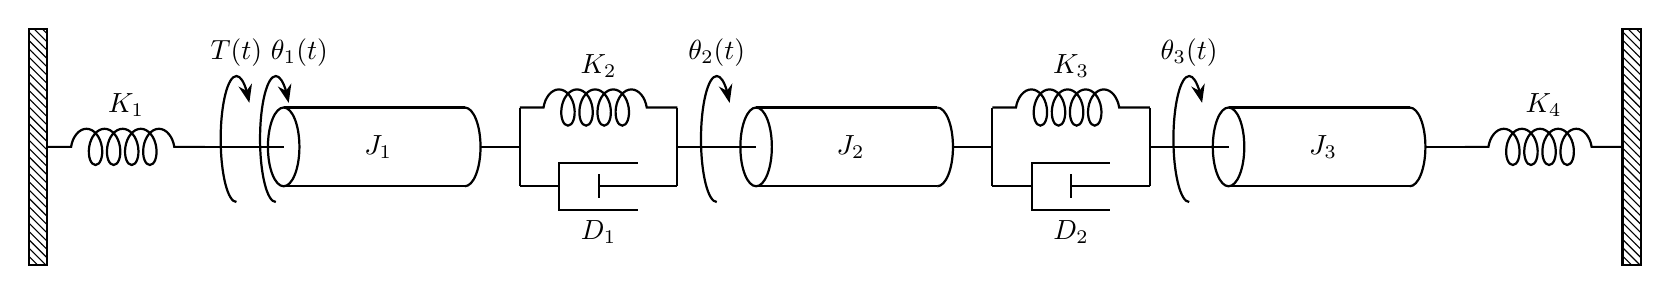
\begin{tikzpicture}[point/.style={coordinate}, >={Stealth}, thick]
        % Left Wall
        \node[wall] (W) at (-0.12,0) {};

        \hspring{0,0}{$K_1$}
        \frbody{(2,0)}

        \draw (6,0.5) -- (6,-0.5);

        \hspring{6,0.5}{$K_2$}
        \bldamper{(6,-0.5)}{$D_1$}

        \draw (8,0.5) -- (8,-0.5);

        \rbody{(8,0)}{$J_2$}{$\theta_2(t)$}

        \draw (12,0.5) -- (12,-0.5);

        \hspring{12,0.5}{$K_3$}
        \bldamper{(12,-0.5)}{$D_2$}
        
        \draw (14,0.5) -- (14,-0.5);

        \rbody{(14,0)}{$J_3$}{$\theta_3(t)$}

        \hspring{18,0}{$K_4$}

        \rwall{20,0}
        
    \end{tikzpicture}
}
\end{center}
\noindent\rule{\textwidth}{1pt}

\vspace{12pt}

\noindent\textbf{\textit{Given:}}
\[
\begin{aligned}
J_1 &= 1\, \text{kg}\cdot\text{m}^2 & K_1 &= 2\, \text{N}\cdot\text{m/rad} & D_1 &= 1\, \text{N}\cdot\text{m}\cdot\text{s/rad} \\
J_2 &= 2\, \text{kg}\cdot\text{m}^2 & K_2 &= 3\, \text{N}\cdot\text{m/rad} & D_2 &= 1\, \text{N}\cdot\text{m}\cdot\text{s/rad} \\
J_3 &= 1\, \text{kg}\cdot\text{m}^2 & K_3 &= 1\, \text{N}\cdot\text{m/rad} & & \\
& & K_4 &= 1\, \text{N}\cdot\text{m/rad} & & 
\end{aligned}
\]

\vspace{12pt}

\noindent \textbf{\textit{Required:}}
\[
G(s) = \frac{\theta_3(s)}{T(s)}
\]

\vspace{12pt}

\noindent \textbf{\textit{Solution:}}\\

% Start of Solution
\begin{enumerate}[label=(\alph*),itemindent=*, itemindent=*, leftmargin=*, nolistsep]
    
    \item Draw the Free Body Diagrams of the provided masses
\vspace{10pt}
    \begin{center}
            \textbf{Free Body Diagram at $J_1$} \\[6pt]
            \vspace{15pt}
            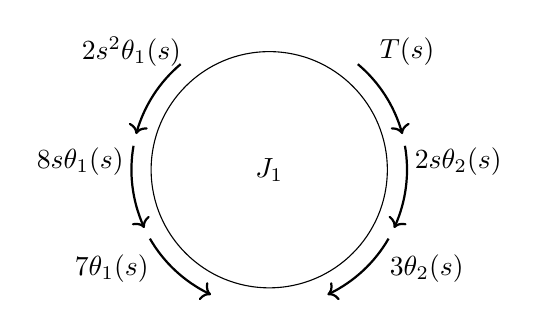
\begin{tikzpicture}
                % Circle
                \draw (0,0) circle (1.5);
                \node at (0,0) {$J_1$};
                % Left-hand Arrows
                \draw[->, thick] (0,0) ++(130:1.75) arc[start angle=130, end angle=165, radius=1.75];
                \node at (-1.75,1.5){$2s^2\theta_1(s)$};
                \draw[->, thick] (0,0) ++(170:1.75) arc[start angle=170, end angle=205, radius=1.75];
                \node at (-2.4,0.1){$8s\theta_1(s)$};
                \draw[->, thick] (0,0) ++(210:1.75) arc[start angle=210, end angle=245, radius=1.75];
                \node at (-2,-1.25){$7\theta_1(s)$};
                % Right-hand Arrows
                \draw[->, thick] (0,0) ++(50:1.75) arc[start angle=50, end angle=15, radius=1.75];
                \node at (1.75,1.5){$T(s)$};
                \draw[->, thick] (0,0) ++(10:1.75) arc[start angle=10, end angle=-25, radius=1.75];
                \node at (2.4,0.1){$2s\theta_2(s)$};
                \draw[->, thick] (0,0) ++(-30:1.75) arc[start angle=-30, end angle=-65, radius=1.75];
                \node at (2,-1.25){$3\theta_2(s)$};
            \end{tikzpicture}
    
            % Equations under J1
            \vspace{15pt}
    
            $\sum T_0 = 0 \quad\text{(clockwise, +)}$ \\ \vspace{10pt}
            $T(s) - (2s^2 + 8s + 7)\theta_1(s) + (2s + 3)\theta_2(s) = 0$ \\ \vspace{10pt}
            $T(s) = (2s^2 + 8s + 7)\theta_1(s) - (2s + 3)\theta_2(s)$

    \end{center}

\vspace{15pt}
    \begin{center}
        %---------------- RIGHT SIDE: J2 ----------------%
            \textbf{Free Body Diagram at $J_2$} \\[6pt]
            \vspace{15pt}
            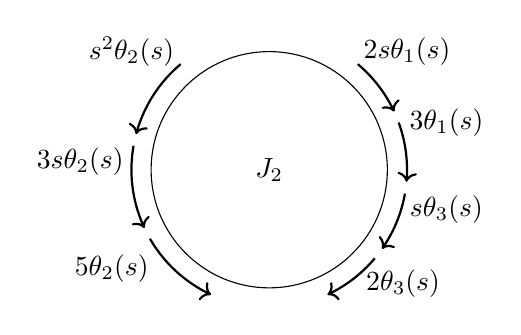
\begin{tikzpicture}
                % Circle
                \draw (0,0) circle (1.5);
                \node at (0,0) {$J_2$};
                % Left-hand Arrows
                \draw[->, thick] (0,0) ++(130:1.75) arc[start angle=130, end angle=165, radius=1.75];
                \node at (-1.75,1.5){$s^2\theta_2(s)$};
                \draw[->, thick] (0,0) ++(170:1.75) arc[start angle=170, end angle=205, radius=1.75];
                \node at (-2.4,0.1){$3s\theta_2(s)$};
                \draw[->, thick] (0,0) ++(210:1.75) arc[start angle=210, end angle=245, radius=1.75];
                \node at (-2,-1.25){$5\theta_2(s)$};
                % Right-hand Arrows
                \draw[->, thick] (0,0) ++(50:1.75) arc[start angle=50, end angle=25, radius=1.75];
                \node at (1.75,1.5){$2s\theta_1(s)$};
                \draw[->, thick] (0,0) ++(20:1.75) arc[start angle=20, end angle=-5, radius=1.75];
                \node at (2.25,0.6){$3\theta_1(s)$};
                \draw[->, thick] (0,0) ++(-10:1.75) arc[start angle=-10, end angle=-35, radius=1.75];
                \node at (2.25,-0.5){$s\theta_3(s)$};
                \draw[->, thick] (0,0) ++(-40:1.75) arc[start angle=-40, end angle=-65, radius=1.75];
                \node at (1.7,-1.45){$2\theta_3(s)$};
            \end{tikzpicture}
    
            % Equations under J2
    
    \vspace{15pt}
    

        $\sum T_0 = 0 \quad\text{(clockwise, +)}$ \\ \vspace{10pt}
        $0 = -(2s + 3)\theta_1(s) - (s^2 + 3s + 5)\theta_2(s) + (s + 2)\theta_3(s)$\\ \vspace{10pt}
        $0 = (2s + 3)\theta_1(s) + (s^2 + 3s + 5)\theta_2(s) - (s + 2)\theta_3(s)$

    \end{center}

    \vspace{15pt}
    \begin{center}
            \textbf{Free Body Diagram at $J_3$} \\[6pt]
            \vspace{15pt}
            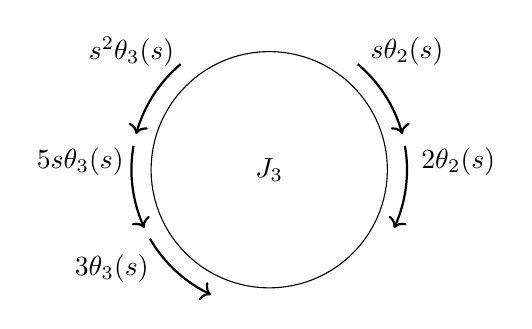
\begin{tikzpicture}
                % Circle
                \draw (0,0) circle (1.5);
                \node at (0,0) {$J_3$};
                % Left-hand Arrows
                \draw[->, thick] (0,0) ++(130:1.75) arc[start angle=130, end angle=165, radius=1.75];
                \node at (-1.75,1.5){$s^2\theta_3(s)$};
                \draw[->, thick] (0,0) ++(170:1.75) arc[start angle=170, end angle=205, radius=1.75];
                \node at (-2.4,0.1){$5s\theta_3(s)$};
                \draw[->, thick] (0,0) ++(210:1.75) arc[start angle=210, end angle=245, radius=1.75];
                \node at (-2,-1.25){$3\theta_3(s)$};
                % Right-hand Arrows
                \draw[->, thick] (0,0) ++(50:1.75) arc[start angle=50, end angle=15, radius=1.75];
                \node at (1.75,1.5){$s\theta_2(s)$};
                \draw[->, thick] (0,0) ++(10:1.75) arc[start angle=10, end angle=-25, radius=1.75];
                \node at (2.4,0.1){$2\theta_2(s)$};
            \end{tikzpicture}
    
            % Equations under J3
            \vspace{15pt}
    
            $\sum T_0 = 0 \quad\text{(clockwise, +)}$ \\ \vspace{10pt}
            $0 = -(s + 2)\theta_2(s) - (s^2 + 5s + 3)\theta_3(s)$ \\ \vspace{10pt}
            $0 = (s + 2)\theta_2(s) + (s^2 + 5s + 3)\theta_3(s)$ 

    \end{center}
\vspace{15pt}
    \item Write the displacement equations and provide the matrix form
\begin{center}
    T(s) $= (2s^2 + 8s + 7)\theta_1(s) - (2s + 3)\theta_2(s)$\\
    0 $= (2s + 3)\theta_1(s) + (s^2 + 3s + 5)\theta_2(s) - (s + 2)\theta_3(s)$\\
    0 $= (s + 2)\theta_2(s) + (s^2 + 5s + 3)\theta_3(s)$\\
    \[
        \begin{bmatrix}
        (2s^2 + 8s + 7) & -(2s + 3) & 0\\
        (2s + 3) & (s^2 + 3s + 5) & -(s + 2)\\
        0 & (s + 2) & (s^2 + 5s + 3)\\
        \end{bmatrix}
        \begin{bmatrix}
        \theta_1(s) \\
        \theta_2(s) \\
        \theta_3(s)
        \end{bmatrix}
        =
        \begin{bmatrix}
        T(s)\\
        0\\
        0
        \end{bmatrix}
    \]\\
\end{center}
\vspace{15pt}
    \item Apply Cramer's Rule to get the value of the Transfer Function
\begin{center}
    \[
        \theta_3(s) = 
            \frac{\begin{vmatrix}
                (2s^2 + 8s + 7) & -(2s + 3) & T(s)\\
                (2s + 3) & (s^2 + 3s + 5) & 0\\
                0 & (s + 2) & 0\\
            \end{vmatrix}
        }{\begin{vmatrix}
                (2s^2 + 8s + 7) & -(2s + 3) & 0\\
                (2s + 3) & (s^2 + 3s + 5) & -(s + 2)\\
                0 & (s + 2) & (s^2 + 5s + 3)\\
            \end{vmatrix}
        }
    \]
    \[
    \theta_3(s) = \frac{(2s^2 + 7s + 6)T(s)}{2s^6 + 24s^5 + 123s^4 + 356s^3 + 591s^2 + 499s + 160}
    \] 

    \[
    \boxed{\frac{\theta_3(s)}{T(s)} = \frac{2s^2 + 7s + 6}{2s^6 + 24s^5 + 123s^4 + 356s^3 + 591s^2 + 499s + 160}}
    \] 

\end{center}
\end{enumerate}

% Problem 18 - Rotational Mechanical System

\newpage
  \setcounter{page}{29}  
\noindent\rule{\textwidth}{1pt}
\noindent\textbf{Problem 18} \hfill
\\For the rotational mechanical system shown in the diagram below, determine the transfer function $G(s)=\theta_3(s)/T(s)$.\\
% P6 Figure
\begin{center}
\resizebox{\textwidth}{!}{%
    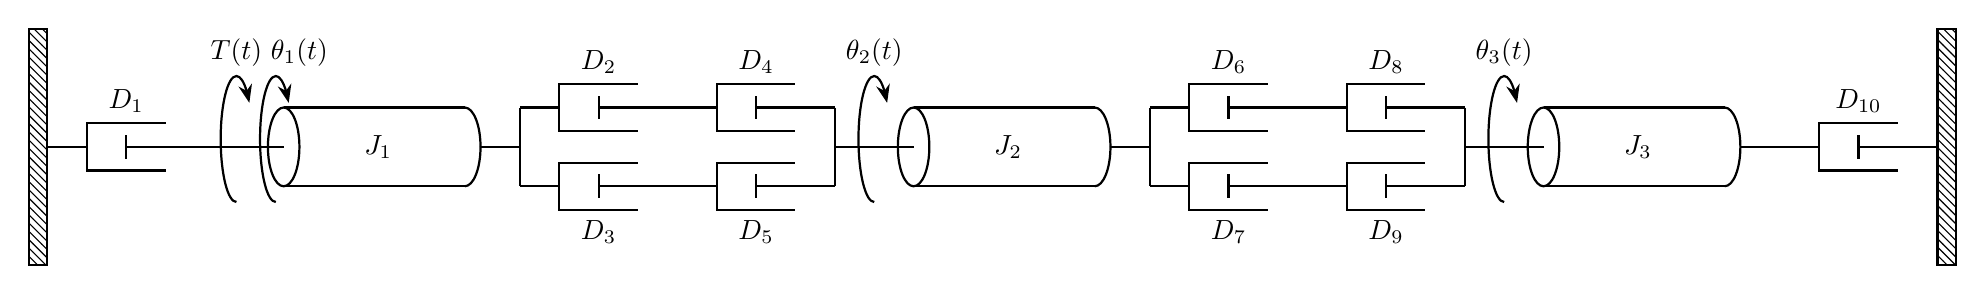
\begin{tikzpicture}[point/.style={coordinate}, >={Stealth}, thick]
        % Left Wall
        \node[wall] (W) at (-0.12,0) {};
        \hdamper{(0,0)}{$D_1$}
        
        \frbody{(2,0)}
        \draw (6,0.5) -- (6,-0.5);
        \hdamper{(6,0.5)}{$D_2$}
        \hdamper{(8,0.5)}{$D_4$}
        \bldamper{(6,-0.5)}{$D_3$}
        \bldamper{(8,-0.5)}{$D_5$}
        \draw(10,0.5) -- (10,-0.5);

        \rbody{(10,0)}{$J_2$}{$\theta _2(t)$}
        \draw (14,0.5) -- (14,-0.5);
        \hdamper{(14,0.5)}{$D_6$}
        \hdamper{(16,0.5)}{$D_8$}
        \bldamper{(14,-0.5)}{$D_7$}
        \bldamper{(16,-0.5)}{$D_9$}
        \draw(18,0.5) -- (18,-0.5);

        \rbody{(18,0)}{$J_3$}{$\theta _3(t)$}
        \hdamper{(22,0)}{$D_{10}$}

        \rwall{24,0}   
    \end{tikzpicture}
}
\end{center}
\noindent\rule{\textwidth}{1pt}

\vspace{12pt}

\noindent\textbf{\textit{Given:}}
\[
\begin{aligned}
J_1 &= 1\, \text{kg}\cdot\text{m}^2 & D_1 &= 1\, \text{N}\cdot\text{m}\cdot\text{s/rad} \\
J_2 &= 1\, \text{kg}\cdot\text{m}^2 & D_2 &= 1\, \text{N}\cdot\text{m}\cdot\text{s/rad} \\
J_3 &= 1\, \text{kg}\cdot\text{m}^2 & D_3 &= 1\, \text{N}\cdot\text{m}\cdot\text{s/rad} \\
& & D_4 &= 1\, \text{N}\cdot\text{m}\cdot\text{s/rad} \\
& & D_5 &= 1\, \text{N}\cdot\text{m}\cdot\text{s/rad} \\
& & D_6 &= 1\, \text{N}\cdot\text{m}\cdot\text{s/rad} \\
& & D_7 &= 1\, \text{N}\cdot\text{m}\cdot\text{s/rad} \\
& & D_8 &= 1\, \text{N}\cdot\text{m}\cdot\text{s/rad} \\
& & D_9 &= 1\, \text{N}\cdot\text{m}\cdot\text{s/rad} \\
& & D_{10} &= 1\, \text{N}\cdot\text{m}\cdot\text{s/rad}
\end{aligned}
\]

\vspace{12pt}

\noindent \textbf{\textit{Required:}}
\[
G(s) = \frac{\theta_3(s)}{T(s)}
\]

\vspace{12pt}

\noindent \textbf{\textit{Solution:}}\\

\begin{enumerate}[label=(\alph*),itemindent=*, leftmargin=*, nolistsep]
    
    \item Draw the Free Body Diagrams of the provided masses
\vspace{10pt}
    \begin{center}
            \textbf{Free Body Diagram at $J_1$} \\[6pt]
            \vspace{15pt}
            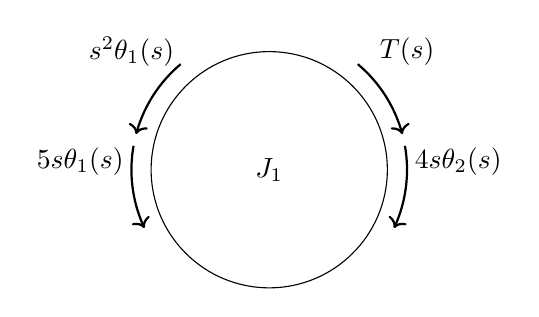
\begin{tikzpicture}
                \draw (0,0) circle (1.5);
                \node at (0,0) {$J_1$};
                \draw[->, thick] (0,0) ++(130:1.75) arc[start angle=130, end angle=165, radius=1.75];
                \node at (-1.75,1.5){$s^2\theta_1(s)$};
                \draw[->, thick] (0,0) ++(170:1.75) arc[start angle=170, end angle=205, radius=1.75];
                \node at (-2.4,0.1){$5s\theta_1(s)$};
                \draw[->, thick] (0,0) ++(50:1.75) arc[start angle=50, end angle=15, radius=1.75];
                \node at (1.75,1.5){$T(s)$};
                \draw[->, thick] (0,0) ++(10:1.75) arc[start angle=10, end angle=-25, radius=1.75];
                \node at (2.4,0.1){$4s\theta_2(s)$};
            \end{tikzpicture}
    
            \vspace{15pt}
    
            $\sum T_0 = 0 \quad\text{(clockwise, +)}$ \\ \vspace{10pt}
            $T(s) - (s^2 + 5s)\theta_1(s) + 4s\theta_2(s) = 0$ \\ \vspace{10pt}
            $T(s) = (s^2 + 5s)\theta_1(s) - 4s\theta_2(s)$

    \end{center}

\vspace{15pt}
    \begin{center}
            \textbf{Free Body Diagram at $J_2$} \\[6pt]
            \vspace{15pt}
            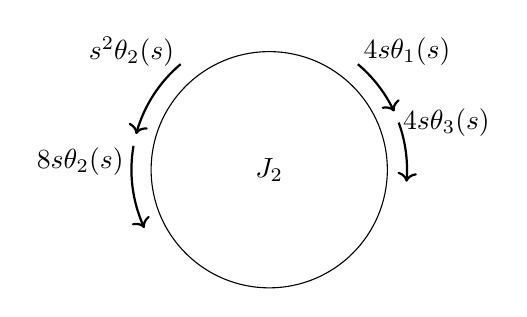
\begin{tikzpicture}
                \draw (0,0) circle (1.5);
                \node at (0,0) {$J_2$};
                \draw[->, thick] (0,0) ++(130:1.75) arc[start angle=130, end angle=165, radius=1.75];
                \node at (-1.75,1.5){$s^2\theta_2(s)$};
                \draw[->, thick] (0,0) ++(170:1.75) arc[start angle=170, end angle=205, radius=1.75];
                \node at (-2.4,0.1){$8s\theta_2(s)$};
                \draw[->, thick] (0,0) ++(50:1.75) arc[start angle=50, end angle=25, radius=1.75];
                \node at (1.75,1.5){$4s\theta_1(s)$};
                \draw[->, thick] (0,0) ++(20:1.75) arc[start angle=20, end angle=-5, radius=1.75];
                \node at (2.25,0.6){$4s\theta_3(s)$};
            \end{tikzpicture}
    
    \vspace{15pt}
    
        $\sum T_0 = 0 \quad\text{(clockwise, +)}$ \\ \vspace{10pt}
        $0 = 4s\theta_1(s) - (s^2 + 8s)\theta_2(s) + 4s\theta_3(s)$\\ \vspace{10pt}
        $0 = -4s\theta_1(s) + (s^2 + 8s)\theta_2(s) - 4s\theta_3(s)$

    \end{center}

    \vspace{15pt}
    \begin{center}
            \textbf{Free Body Diagram at $J_3$} \\[6pt]
            \vspace{15pt}
            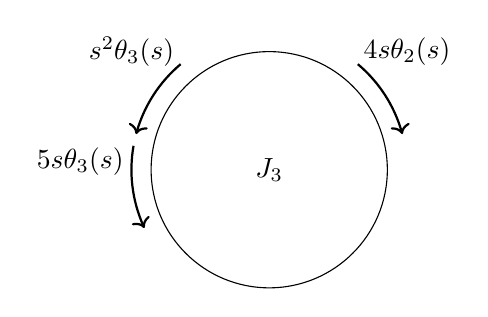
\begin{tikzpicture}
                \draw (0,0) circle (1.5);
                \node at (0,0) {$J_3$};
                \draw[->, thick] (0,0) ++(130:1.75) arc[start angle=130, end angle=165, radius=1.75];
                \node at (-1.75,1.5){$s^2\theta_3(s)$};
                \draw[->, thick] (0,0) ++(170:1.75) arc[start angle=170, end angle=205, radius=1.75];
                \node at (-2.4,0.1){$5s\theta_3(s)$};
                \draw[->, thick] (0,0) ++(50:1.75) arc[start angle=50, end angle=15, radius=1.75];
                \node at (1.75,1.5){$4s\theta_2(s)$};
            \end{tikzpicture}
    
            \vspace{15pt}
    
            $\sum T_0 = 0 \quad\text{(clockwise, +)}$ \\ \vspace{10pt}
            $0 = 4s\theta_2(s) - (s^2 + 5s)\theta_3(s)$ \\ \vspace{10pt}
            $0 = -4s\theta_2(s) + (s^2 + 5s)\theta_3(s)$ 

    \end{center}
\vspace{15pt}
    \item Write the displacement equations and provide the matrix form
\begin{center}
    T(s) $= (s^2 + 5s)\theta_1(s) - 4s\theta_2(s)$\\
    0 $= -4s\theta_1(s) + (s^2 + 8s)\theta_2(s) - 4s\theta_3(s)$\\
    0 $= -4s\theta_2(s) + (s^2 + 5s)\theta_3(s)$\\
    \[
        \begin{bmatrix}
        (s^2 + 5s) & -4s & 0\\
        -4s & (s^2 + 8s) & -4s\\
        0 & -4s & (s^2 + 5s)\\
        \end{bmatrix}
        \begin{bmatrix}
        \theta_1(s) \\
        \theta_2(s) \\
        \theta_3(s)
        \end{bmatrix}
        =
        \begin{bmatrix}
        T(s)\\
        0\\
        0
        \end{bmatrix}
    \]\\
\end{center}
\vspace{15pt}
    \item Apply Cramer's Rule to get the value of the Transfer Function
\begin{center}
    \[
        \theta_3(s) = 
            \frac{\begin{vmatrix}
                (s^2 + 5s) & -4s & T(s)\\
                -4s & (s^2 + 8s) & 0\\
                0 & -4s & 0\\
            \end{vmatrix}
        }{\begin{vmatrix}
                (s^2 + 5s) & -4s & 0\\
                -4s & (s^2 + 8s) & -4s\\
                0 & -4s & (s^2 + 5s)\\
            \end{vmatrix}
        }
    \]
    \[
    \theta_3(s) = \frac{16s^2 T(s)}{s^6 + 18s^5 + 73s^4 + 40s^3}
    \] 

    \[
    \boxed{\frac{\theta_3(s)}{T(s)} = \frac{16s^2}{s^6 + 18s^5 + 73s^4 + 40s^3}}
    \] 

\end{center}
\end{enumerate}

% Problem 19 - Rotational Mechanical System

\newpage
  \setcounter{page}{31}  
\noindent\rule{\textwidth}{1pt}
\noindent\textbf{Problem 19} \hfill
\\For the rotational mechanical system shown in the diagram below, determine the transfer function $G(s)=\theta_3(s)/T(s)$.\\
% P6 Figure
\begin{center}
\resizebox{\textwidth}{!}{%
    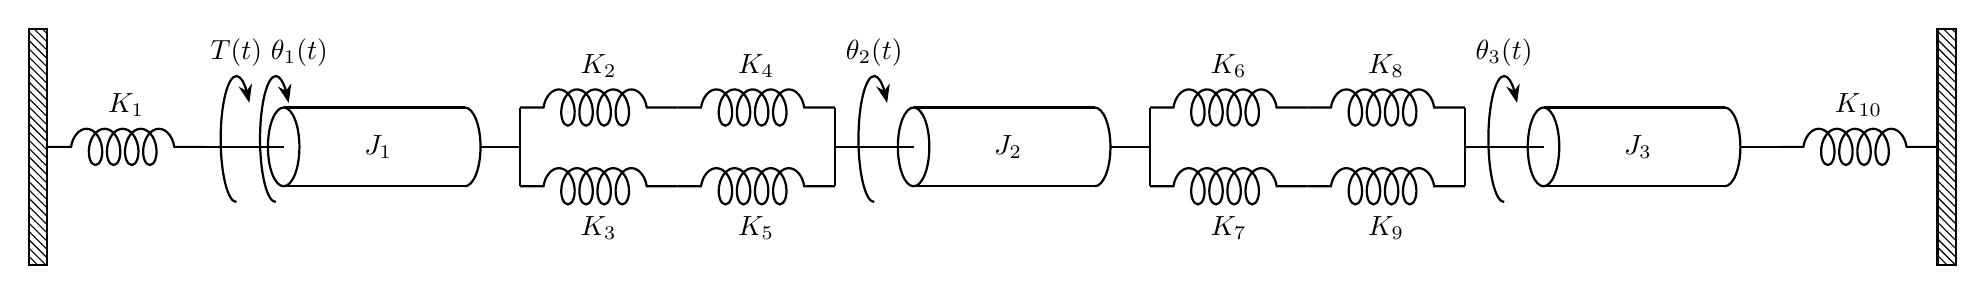
\begin{tikzpicture}[point/.style={coordinate}, >={Stealth}, thick]
        % Left Wall
        \node[wall] (W) at (-0.12,0) {};
        \hspring{0,0}{$K_1$}
        
        \frbody{(2,0)}
        \draw(6,0.5) -- (6,-0.5);
        \hspring{6,0.5}{$K_2$}
        \blspring{6,-0.5}{$K_3$}
        \hspring{8,0.5}{$K_4$}
        \blspring{8,-0.5}{$K_5$}
        \draw(10,0.5)--(10,-0.5);
        
        \rbody{(10,0)}{$J_2$}{$\theta _2(t)$}
        \draw (14,0.5)--(14,-0.5);
        \hspring{14,0.5}{$K_6$}
        \blspring{14,-0.5}{$K_7$}
        \hspring{16,0.5}{$K_8$}
        \blspring{16,-0.5}{$K_9$}
        \draw (18,0.5)--(18,-0.5);

        \rbody{(18,0)}{$J_3$}{$\theta _3(t)$}
        
        \hspring{22,0}{$K_{10}$}

        \rwall{24,0}   
    \end{tikzpicture}
}
\end{center}
\noindent\rule{\textwidth}{1pt}
\vspace{12pt}

\noindent\textbf{\textit{Given:}}
\[
\begin{aligned}
J_1 &= 1\, \text{kg}\cdot\text{m}^2 & K_1 &= 1\, \text{N}\cdot\text{m/rad} & K_6 &= 1\, \text{N}\cdot\text{m/rad} \\
J_2 &= 1\, \text{kg}\cdot\text{m}^2 & K_2 &= 1\, \text{N}\cdot\text{m/rad} & K_7 &= 1\, \text{N}\cdot\text{m/rad} \\
J_3 &= 1\, \text{kg}\cdot\text{m}^2 & K_3 &= 1\, \text{N}\cdot\text{m/rad} & K_8 &= 1\, \text{N}\cdot\text{m/rad} \\
& & K_4 &= 1\, \text{N}\cdot\text{m/rad} & K_9 &= 1\, \text{N}\cdot\text{m/rad} \\
& & K_5 &= 1\, \text{N}\cdot\text{m/rad} & K_{10} &= 1\, \text{N}\cdot\text{m/rad}
\end{aligned}
\]

\vspace{12pt}

\noindent \textbf{\textit{Required:}}
\[
G(s) = \frac{\theta_3(s)}{T(s)}
\]

\vspace{12pt}


\noindent \textbf{\textit{Solution:}}\\

\begin{enumerate}[label=(\alph*),itemindent=*, leftmargin=*, nolistsep]
    
    \item Draw the Free Body Diagrams of the provided masses
\vspace{10pt}
    \begin{center}
            \textbf{Free Body Diagram at $J_1$} \\[6pt]
            \vspace{15pt}
            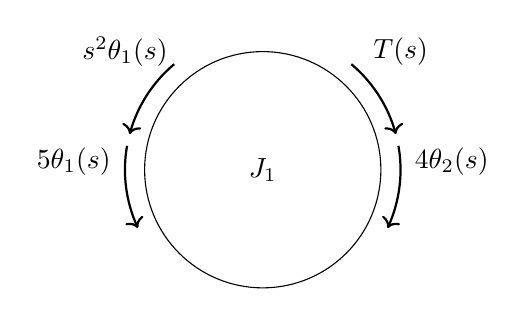
\begin{tikzpicture}
                \draw (0,0) circle (1.5);
                \node at (0,0) {$J_1$};
                \draw[->, thick] (0,0) ++(130:1.75) arc[start angle=130, end angle=165, radius=1.75];
                \node at (-1.75,1.5){$s^2\theta_1(s)$};
                \draw[->, thick] (0,0) ++(170:1.75) arc[start angle=170, end angle=205, radius=1.75];
                \node at (-2.4,0.1){$5\theta_1(s)$};
                \draw[->, thick] (0,0) ++(50:1.75) arc[start angle=50, end angle=15, radius=1.75];
                \node at (1.75,1.5){$T(s)$};
                \draw[->, thick] (0,0) ++(10:1.75) arc[start angle=10, end angle=-25, radius=1.75];
                \node at (2.4,0.1){$4\theta_2(s)$};
            \end{tikzpicture}
    
            \vspace{15pt}
    
            $\sum T_0 = 0 \quad\text{(clockwise, +)}$ \\ \vspace{10pt}
            $T(s) - (s^2 + 5)\theta_1(s) + 4\theta_2(s) = 0$ \\ \vspace{10pt}
            $T(s) = (s^2 + 5)\theta_1(s) - 4\theta_2(s)$

    \end{center}

\vspace{15pt}
    \begin{center}
            \textbf{Free Body Diagram at $J_2$} \\[6pt]
            \vspace{15pt}
            \begin{tikzpicture}
                \draw (0,0) circle (1.5);
                \node at (0,0) {$J_2$};
                \draw[->, thick] (0,0) ++(130:1.75) arc[start angle=130, end angle=165, radius=1.75];
                \node at (-1.75,1.5){$s^2\theta_2(s)$};
                \draw[->, thick] (0,0) ++(170:1.75) arc[start angle=170, end angle=205, radius=1.75];
                \node at (-2.4,0.1){$8\theta_2(s)$};
                \draw[->, thick] (0,0) ++(50:1.75) arc[start angle=50, end angle=25, radius=1.75];
                \node at (1.75,1.5){$4\theta_1(s)$};
                \draw[->, thick] (0,0) ++(20:1.75) arc[start angle=20, end angle=-5, radius=1.75];
                \node at (2.25,0.6){$4\theta_3(s)$};
            \end{tikzpicture}
    
    \vspace{15pt}
        $\sum T_0 = 0 \quad\text{(clockwise, +)}$ \\ \vspace{10pt}
        $0 = 4\theta_1(s) - (s^2 + 8)\theta_2(s) + 4\theta_3(s)$\\ \vspace{10pt}
        $0 = -4\theta_1(s) + (s^2 + 8)\theta_2(s) - 4\theta_3(s)$
    \end{center}

    \vspace{15pt}
    \begin{center}
            \textbf{Free Body Diagram at $J_3$} \\[6pt]
            \vspace{15pt}
            \begin{tikzpicture}
                \draw (0,0) circle (1.5);
                \node at (0,0) {$J_3$};
                \draw[->, thick] (0,0) ++(130:1.75) arc[start angle=130, end angle=165, radius=1.75];
                \node at (-1.75,1.5){$s^2\theta_3(s)$};
                \draw[->, thick] (0,0) ++(170:1.75) arc[start angle=170, end angle=205, radius=1.75];
                \node at (-2.4,0.1){$5\theta_3(s)$};
                \draw[->, thick] (0,0) ++(50:1.75) arc[start angle=50, end angle=15, radius=1.75];
                \node at (1.75,1.5){$4\theta_2(s)$};
            \end{tikzpicture}
    
            \vspace{15pt}
    
            $\sum T_0 = 0 \quad\text{(clockwise, +)}$ \\ \vspace{10pt}
            $0 = 4\theta_2(s) - (s^2 + 5)\theta_3(s)$ \\ \vspace{10pt}
            $0 = -4\theta_2(s) + (s^2 + 5)\theta_3(s)$ 

    \end{center}
\vspace{15pt}
    \item Write the displacement equations and provide the matrix form
\begin{center}
    T(s) $= (s^2 + 5)\theta_1(s) - 4\theta_2(s)$\\
    0 $= -4\theta_1(s) + (s^2 + 8)\theta_2(s) - 4\theta_3(s)$\\
    0 $= -4\theta_2(s) + (s^2 + 5)\theta_3(s)$\\
    \[
        \begin{bmatrix}
        (s^2 + 5) & -4 & 0\\
        -4 & (s^2 + 8) & -4\\
        0 & -4 & (s^2 + 5)\\
        \end{bmatrix}
        \begin{bmatrix}
        \theta_1(s) \\
        \theta_2(s) \\
        \theta_3(s)
        \end{bmatrix}
        =
        \begin{bmatrix}
        T(s)\\
        0\\
        0
        \end{bmatrix}
    \]\\
\end{center}
\vspace{15pt}
    \item Apply Cramer's Rule to get the value of the Transfer Function
\begin{center}
    \[
        \theta_3(s) = 
            \frac{\begin{vmatrix}
                (s^2 + 5) & -4 & T(s)\\
                -4 & (s^2 + 8) & 0\\
                0 & -4 & 0\\
            \end{vmatrix}
        }{\begin{vmatrix}
                (s^2 + 5) & -4 & 0\\
                -4 & (s^2 + 8) & -4\\
                0 & -4 & (s^2 + 5)\\
            \end{vmatrix}
        }
    \]
    \[
    \theta_3(s) = \frac{16 T(s)}{s^6 + 18s^4 + 73s^2 + 40}
    \] 

    \[
    \boxed{\frac{\theta_3(s)}{T(s)} = \frac{16}{s^6 + 18s^4 + 73s^2 + 40}}
    \] 

\end{center}
\end{enumerate}

% Problem 20 - Rotational Mechanical System

\newpage
  \setcounter{page}{33}  
\noindent\rule{\textwidth}{1pt}
\noindent\textbf{Problem 20} \hfill
\\For the rotational mechanical system shown in the diagram below, determine the transfer function $G(s)=\theta_2(s)/T(s)$.\\
% P6 Figure
\begin{center}
\resizebox{\textwidth}{!}{%
    \begin{tikzpicture}[point/.style={coordinate}, >={Stealth}, thick]
        % Left Wall
        \node[wall] (W) at (-0.12,0) {};
        \hspring{0,0.5}{$K_1$}
        \blspring{0,-0.5}{$K_2$}
        \draw(2,0.5)--(2,-0.5);
        \hdamper{(2,0)}{$D_1$}
        \frbody{(4,0)}
        \draw(8,0.5)--(8,-0.5);
        \hdamper{(8,0.5)}{$D_2$}
        \bldamper{(8,-0.5)}{$D_3$}
        \draw(10,0.5)--(10,-0.5);
        \hspring{10,0}{$K_3$}
        \rbody{(12,0)}{$J_2$}{$\theta_2(t)$}
        \hdamper{(16,0)}{$D_4$}
        
        \rwall{18,0}   
    \end{tikzpicture}
}
\end{center}
\noindent\rule{\textwidth}{1pt}
\vspace{12pt}

\noindent\textbf{\textit{Given:}}
\[
\begin{aligned}
J_1 &= 2\, \text{kg}\cdot\text{m}^2 & K_1 &= 4\, \text{N}\cdot\text{m/rad} & D_1 &= 6\, \text{N}\cdot\text{m}\cdot\text{s/rad} \\
J_2 &= 1\, \text{kg}\cdot\text{m}^2 & K_2 &= 5\, \text{N}\cdot\text{m/rad} & D_2 &= 2\, \text{N}\cdot\text{m}\cdot\text{s/rad} \\
& & K_3 &= 3\, \text{N}\cdot\text{m/rad} & D_3 &= 1\, \text{N}\cdot\text{m}\cdot\text{s/rad} \\
& & & & D_4 &= 4\, \text{N}\cdot\text{m}\cdot\text{s/rad} 
\end{aligned}
\]

\vspace{12pt}

\noindent \textbf{\textit{Required:}}
\[
G(s) = \frac{\theta_2(s)}{T(s)}
\]

\vspace{12pt}

\noindent \textbf{\textit{Solution:}}\\

\begin{enumerate}[label=(\alph*),itemindent=*, leftmargin=*, nolistsep]
    
    \item Draw the Free Body Diagrams of the provided masses
\vspace{10pt}
    \begin{center}
            \textbf{Free Body Diagram at $J_1$} \\[6pt]
            \vspace{15pt}
            \begin{tikzpicture}
                \draw (0,0) circle (1.5);
                \node at (0,0) {$J_1$};
                \draw[->, thick] (0,0) ++(130:1.75) arc[start angle=130, end angle=165, radius=1.75];
                \node at (-1.75,1.5){$s^2\theta_1(s)$};
                \draw[->, thick] (0,0) ++(170:1.75) arc[start angle=170, end angle=205, radius=1.75];
                \node at (-2.4,0.1){$3s\theta_1(s)$};
                \draw[->, thick] (0,0) ++(210:1.75) arc[start angle=210, end angle=245, radius=1.75];
                \node at (-2,-1.25){$3\theta_1(s)$};
                \draw[->, thick] (0,0) ++(50:1.75) arc[start angle=50, end angle=15, radius=1.75];
                \node at (1.75,1.5){$T(s)$};
                \draw[->, thick] (0,0) ++(10:1.75) arc[start angle=10, end angle=-25, radius=1.75];
                \node at (2.4,0.1){$2s\theta_2(s)$};
                \draw[->, thick] (0,0) ++(-30:1.75) arc[start angle=-30, end angle=-65, radius=1.75];
                \node at (2,-1.25){$1\theta_2(s)$};
            \end{tikzpicture}
    
            \vspace{15pt}
    
            $\sum T_0 = 0 \quad\text{(clockwise, +)}$ \\ \vspace{10pt}
            $T(s) - (s^2 + 3s + 3)\theta_1(s) + (2s + 1)\theta_2(s) = 0$ \\ \vspace{10pt}
            $T(s) = (s^2 + 3s + 3)\theta_1(s) - (2s + 1)\theta_2(s)$

    \end{center}

\vspace{15pt}
    \begin{center}
            \textbf{Free Body Diagram at $J_2$} \\[6pt]
            \vspace{15pt}
            \begin{tikzpicture}
                \draw (0,0) circle (1.5);
                \node at (0,0) {$J_2$};
                \draw[->, thick] (0,0) ++(130:1.75) arc[start angle=130, end angle=165, radius=1.75];
                \node at (-1.75,1.5){$s^2\theta_2(s)$};
                \draw[->, thick] (0,0) ++(170:1.75) arc[start angle=170, end angle=205, radius=1.75];
                \node at (-2.4,0.1){$3s\theta_2(s)$};
                \draw[->, thick] (0,0) ++(210:1.75) arc[start angle=210, end angle=245, radius=1.75];
                \node at (-2,-1.25){$1\theta_2(s)$};
                \draw[->, thick] (0,0) ++(50:1.75) arc[start angle=50, end angle=25, radius=1.75];
                \node at (1.75,1.5){$2s\theta_1(s)$};
                \draw[->, thick] (0,0) ++(20:1.75) arc[start angle=20, end angle=-5, radius=1.75];
                \node at (2.25,0.6){$1\theta_1(s)$};
            \end{tikzpicture}
    
    \vspace{15pt}
    
        $\sum T_0 = 0 \quad\text{(clockwise, +)}$ \\ \vspace{10pt}
        $0 = (2s + 1)\theta_1(s) - (s^2 + 3s + 1)\theta_2(s)$\\ \vspace{10pt}
        $0 = -(2s + 1)\theta_1(s) + (s^2 + 3s + 1)\theta_2(s)$

    \end{center}

\vspace{15pt}
    \item Write the displacement equations and provide the matrix form
\begin{center}
    T(s) $= (s^2 + 3s + 3)\theta_1(s) - (2s + 1)\theta_2(s)$\\
    0 $= -(2s + 1)\theta_1(s) + (s^2 + 3s + 1)\theta_2(s)$\\
    \[
        \begin{bmatrix}
        (s^2 + 3s + 3) & -(2s + 1) \\
        -(2s + 1) & (s^2 + 3s + 1)
        \end{bmatrix}
        \begin{bmatrix}
        \theta_1(s) \\
        \theta_2(s)
        \end{bmatrix}
        =
        \begin{bmatrix}
        T(s)\\
        0
        \end{bmatrix}
    \]\\
\end{center}
\vspace{15pt}
    \item Apply Cramer's Rule to get the value of the Transfer Function
\begin{center}
    \[
        \theta_2(s) = 
            \frac{\begin{vmatrix}
                (s^2 + 3s + 3) & T(s)\\
                -(2s + 1) & 0
            \end{vmatrix}
        }{\begin{vmatrix}
                (s^2 + 3s + 3) & -(2s + 1) \\
                -(2s + 1) & (s^2 + 3s + 1)
            \end{vmatrix}
        }
    \]
    \[
    \theta_2(s) = \frac{(2s+1)T(s)}{s^4 + 6s^3 + 9s^2 + 8s + 2}
    \] 

    \[
    \boxed{\frac{\theta_2(s)}{T(s)} = \frac{2s+1}{s^4 + 6s^3 + 9s^2 + 8s + 2}}
    \] 

\end{center}
\end{enumerate}

% Problem 21 - Rotational Mechanical System

\newpage
  \setcounter{page}{35}  
\noindent\rule{\textwidth}{1pt}
\noindent\textbf{Problem 21} \hfill
\\For the rotational mechanical system shown in the diagram below, determine the transfer function $G(s)=\theta_2(s)/T(s)$.\\
% P6 Figure
\begin{center}
\resizebox{\textwidth}{!}{%
    \begin{tikzpicture}[point/.style={coordinate}, >={Stealth}, thick]
        % Left Wall
        \node[wall] (W) at (-0.12,0) {};
        
        \hspring{0,0.5}{$K_1$}
        \blspring{0,-0.5}{$K_2$}
        \hspring{2,0.5}{$K_3$}
        \blspring{2,-0.5}{$K_4$}
        \draw(4,0.5)--(4,-0.5);
        
        \frbody{(4,0)}

        \draw (8,0.5)--(8,-0.5);
        \hdamper{(8,0.5)}{$D_1$}
        \bldamper{(8,-0.5)}{$D_2$}
        \hdamper{(10,0.5)}{$D_3$}
        \bldamper{(10,-0.5)}{$D_4$}
        \draw (12,0.5)--(12,-0.5);

        \rbody{(12,0)}{$J_2$}{$\theta _2(t)$}
        \draw(16,0.5) -- (16,-0.5);
        \hspring{16,0.5}{$K_5$}
        \blspring{16,-0.5}{$K_{6}$}
        \hspring{18,0.5}{$K_{7}$}
        \blspring{18,-0.5}{$K_{8}$}
        

        \rwall{20,0}   
    \end{tikzpicture}
}
\end{center}
\noindent\rule{\textwidth}{1pt}
\vspace{12pt}

\noindent\textbf{\textit{Given:}}
\[
\begin{aligned}
J_1 &= 1\, \text{kg}\cdot\text{m}^2 & K_1 &= 1\, \text{N}\cdot\text{m/rad} & K_5 &= 1\, \text{N}\cdot\text{m/rad} & D_1 &= 1\, \text{N}\cdot\text{m}\cdot\text{s/rad} \\
J_2 &= 1\, \text{kg}\cdot\text{m}^2 & K_2 &= 1\, \text{N}\cdot\text{m/rad} & K_6 &= 1\, \text{N}\cdot\text{m/rad} & D_2 &= 1\, \text{N}\cdot\text{m}\cdot\text{s/rad} \\
& & K_3 &= 1\, \text{N}\cdot\text{m/rad} & K_7 &= 1\, \text{N}\cdot\text{m/rad} & D_3 &= 1\, \text{N}\cdot\text{m}\cdot\text{s/rad} \\
& & K_4 &= 1\, \text{N}\cdot\text{m/rad} & K_8 &= 1\, \text{N}\cdot\text{m/rad} & D_4 &= 1\, \text{N}\cdot\text{m}\cdot\text{s/rad}
\end{aligned}
\]

\vspace{12pt}

\noindent \textbf{\textit{Required:}}
\[
G(s) = \frac{\theta_2(s)}{T(s)}
\]

\vspace{12pt}

\noindent \textbf{\textit{Solution:}}\\
\begin{enumerate}[label=(\alph*),itemindent=*, leftmargin=*, nolistsep]
    
    \item Draw the Free Body Diagrams of the provided masses
\vspace{10pt}
    \begin{center}
            \textbf{Free Body Diagram at $J_1$} \\[6pt]
            \vspace{15pt}
            \begin{tikzpicture}
                \draw (0,0) circle (1.5);
                \node at (0,0) {$J_1$};
                \draw[->, thick] (0,0) ++(130:1.75) arc[start angle=130, end angle=165, radius=1.75];
                \node at (-1.75,1.5){$s^2\theta_1(s)$};
                \draw[->, thick] (0,0) ++(170:1.75) arc[start angle=170, end angle=205, radius=1.75];
                \node at (-2.4,0.1){$4s\theta_1(s)$};
                \draw[->, thick] (0,0) ++(210:1.75) arc[start angle=210, end angle=245, radius=1.75];
                \node at (-2,-1.25){$4\theta_1(s)$};
                \draw[->, thick] (0,0) ++(50:1.75) arc[start angle=50, end angle=15, radius=1.75];
                \node at (1.75,1.5){$T(s)$};
                \draw[->, thick] (0,0) ++(10:1.75) arc[start angle=10, end angle=-25, radius=1.75];
                \node at (2.4,0.1){$4s\theta_2(s)$};
            \end{tikzpicture}
    
            \vspace{15pt}
    
            $\sum T_0 = 0 \quad\text{(clockwise, +)}$ \\ \vspace{10pt}
            $T(s) - (s^2 + 4s + 4)\theta_1(s) + 4s\theta_2(s) = 0$ \\ \vspace{10pt}
            $T(s) = (s^2 + 4s + 4)\theta_1(s) - 4s\theta_2(s)$

    \end{center}

\vspace{15pt}
    \begin{center}
            \textbf{Free Body Diagram at $J_2$} \\[6pt]
            \vspace{15pt}
            \begin{tikzpicture}
                \draw (0,0) circle (1.5);
                \node at (0,0) {$J_2$};
                \draw[->, thick] (0,0) ++(130:1.75) arc[start angle=130, end angle=165, radius=1.75];
                \node at (-1.75,1.5){$s^2\theta_2(s)$};
                \draw[->, thick] (0,0) ++(170:1.75) arc[start angle=170, end angle=205, radius=1.75];
                \node at (-2.4,0.1){$4s\theta_2(s)$};
                \draw[->, thick] (0,0) ++(210:1.75) arc[start angle=210, end angle=245, radius=1.75];
                \node at (-2,-1.25){$4\theta_2(s)$};
                \draw[->, thick] (0,0) ++(50:1.75) arc[start angle=50, end angle=25, radius=1.75];
                \node at (1.75,1.5){$4s\theta_1(s)$};
            \end{tikzpicture}
    
    \vspace{15pt}
    
        $\sum T_0 = 0 \quad\text{(clockwise, +)}$ \\ \vspace{10pt}
        $0 = 4s\theta_1(s) - (s^2 + 4s + 4)\theta_2(s)$\\ \vspace{10pt}
        $0 = -4s\theta_1(s) + (s^2 + 4s + 4)\theta_2(s)$

    \end{center}

\vspace{15pt}
    \item Write the displacement equations and provide the matrix form
\begin{center}
    T(s) $= (s^2 + 4s + 4)\theta_1(s) - 4s\theta_2(s)$\\
    0 $= -4s\theta_1(s) + (s^2 + 4s + 4)\theta_2(s)$\\
    \[
        \begin{bmatrix}
        (s^2 + 4s + 4) & -4s \\
        -4s & (s^2 + 4s + 4)
        \end{bmatrix}
        \begin{bmatrix}
        \theta_1(s) \\
        \theta_2(s)
        \end{bmatrix}
        =
        \begin{bmatrix}
        T(s)\\
        0
        \end{bmatrix}
    \]\\
\end{center}
\vspace{15pt}
    \item Apply Cramer's Rule to get the value of the Transfer Function
\begin{center}
    \[
        \theta_2(s) = 
            \frac{\begin{vmatrix}
                (s^2 + 4s + 4) & T(s)\\
                -4s & 0
            \end{vmatrix}
        }{\begin{vmatrix}
                (s^2 + 4s + 4) & -4s \\
                -4s & (s^2 + 4s + 4)
            \end{vmatrix}
        }
    \]
    \[
    \theta_2(s) = \frac{4s T(s)}{s^4 + 8s^3 + 8s^2 + 32s + 16}
    \] 

    \[
    \boxed{\frac{\theta_2(s)}{T(s)} = \frac{4s}{s^4 + 8s^3 + 8s^2 + 32s + 16}}
    \] 

\end{center}
\end{enumerate}

% Problem 22 - Rotational Mechanical System

\newpage
  \setcounter{page}{37}  
\noindent\rule{\textwidth}{1pt}
\noindent\textbf{Problem 22} \hfill
\\For the rotational mechanical system shown in the diagram below, determine the transfer function $G(s)=\theta_2(s)/T(s)$.\\
% P6 Figure
\begin{center}
\resizebox{\textwidth}{!}{%
    \begin{tikzpicture}[point/.style={coordinate}, >={Stealth}, thick]
        % Left Wall
        \node[wall] (W) at (-0.12,0) {};
        
        \hdamper{(0,0.5)}{$D_1$}
        \bldamper{(0,-0.5)}{$D_2$}
        \hdamper{(2,0.5)}{$D_3$}
        \bldamper{(2,-0.5)}{$D_4$}
        \draw(4,0.5)--(4,-0.5);
        
        \frbody{(4,0)}
        \draw (8,0.5)--(8,-0.5);
        \hspring{8,0.5}{$K_1$}
        \blspring{8,-0.5}{$K_2$}
        \hspring{10,0.5}{$K_3$}
        \blspring{10,-0.5}{$K_4$}
        \draw (12,0.5)--(12,-0.5);

        \rbody{(12,0)}{$J_2$}{$\theta _2(t)$}
        \draw(16,0.5) -- (16,-0.5);
        \hdamper{(16,0.5)}{$D_5$}
        \bldamper{(16,-0.5)}{$D_{6}$}
        \hdamper{(18,0.5)}{$D_{7}$}
        \bldamper{(18,-0.5)}{$D_{8}$}
        

        \rwall{20,0}   
    \end{tikzpicture}
}
\end{center}
\noindent\rule{\textwidth}{1pt}

\vspace{12pt}

\noindent\textbf{\textit{Given:}}
\[
\begin{aligned}
J_1 &= 1\, \text{kg}\cdot\text{m}^2 & K_1 &= 1\, \text{N}\cdot\text{m/rad} & D_1 &= 1\, \text{N}\cdot\text{m}\cdot\text{s/rad} & D_5 &= 1\, \text{N}\cdot\text{m}\cdot\text{s/rad} \\
J_2 &= 1\, \text{kg}\cdot\text{m}^2 & K_2 &= 1\, \text{N}\cdot\text{m/rad} & D_2 &= 1\, \text{N}\cdot\text{m}\cdot\text{s/rad} & D_6 &= 1\, \text{N}\cdot\text{m}\cdot\text{s/rad} \\
& & K_3 &= 1\, \text{N}\cdot\text{m/rad} & D_3 &= 1\, \text{N}\cdot\text{m}\cdot\text{s/rad} & D_7 &= 1\, \text{N}\cdot\text{m}\cdot\text{s/rad} \\
& & K_4 &= 1\, \text{N}\cdot\text{m/rad} & D_4 &= 1\, \text{N}\cdot\text{m}\cdot\text{s/rad} & D_8 &= 1\, \text{N}\cdot\text{m}\cdot\text{s/rad}
\end{aligned}
\]

\vspace{12pt}

\noindent \textbf{\textit{Required:}}
\[
G(s) = \frac{\theta_2(s)}{T(s)}
\]

\vspace{12pt}

\noindent \textbf{\textit{Solution:}}\\
\begin{enumerate}[label=(\alph*),itemindent=*, leftmargin=*, nolistsep]
    
    \item Draw the Free Body Diagrams of the provided masses
\vspace{10pt}
    \begin{center}
            \textbf{Free Body Diagram at $J_1$} \\[6pt]
            \vspace{15pt}
            \begin{tikzpicture}
                \draw (0,0) circle (1.5);
                \node at (0,0) {$J_1$};
                \draw[->, thick] (0,0) ++(130:1.75) arc[start angle=130, end angle=165, radius=1.75];
                \node at (-1.75,1.5){$s^2\theta_1(s)$};
                \draw[->, thick] (0,0) ++(170:1.75) arc[start angle=170, end angle=205, radius=1.75];
                \node at (-2.4,0.1){$4s\theta_1(s)$};
                \draw[->, thick] (0,0) ++(210:1.75) arc[start angle=210, end angle=245, radius=1.75];
                \node at (-2,-1.25){$4\theta_1(s)$};
                \draw[->, thick] (0,0) ++(50:1.75) arc[start angle=50, end angle=15, radius=1.75];
                \node at (1.75,1.5){$T(s)$};
                \draw[->, thick] (0,0) ++(10:1.75) arc[start angle=10, end angle=-25, radius=1.75];
                \node at (2.4,0.1){$4s\theta_2(s)$};
            \end{tikzpicture}
    
            \vspace{15pt}
    
            $\sum T_0 = 0 \quad\text{(clockwise, +)}$ \\ \vspace{10pt}
            $T(s) - (s^2 + 4s + 4)\theta_1(s) + 4s\theta_2(s) = 0$ \\ \vspace{10pt}
            $T(s) = (s^2 + 4s + 4)\theta_1(s) - 4s\theta_2(s)$

    \end{center}

\vspace{15pt}
    \begin{center}
            \textbf{Free Body Diagram at $J_2$} \\[6pt]
            \vspace{15pt}
            \begin{tikzpicture}
                \draw (0,0) circle (1.5);
                \node at (0,0) {$J_2$};
                \draw[->, thick] (0,0) ++(130:1.75) arc[start angle=130, end angle=165, radius=1.75];
                \node at (-1.75,1.5){$s^2\theta_2(s)$};
                \draw[->, thick] (0,0) ++(170:1.75) arc[start angle=170, end angle=205, radius=1.75];
                \node at (-2.4,0.1){$4s\theta_2(s)$};
                \draw[->, thick] (0,0) ++(210:1.75) arc[start angle=210, end angle=245, radius=1.75];
                \node at (-2,-1.25){$4\theta_2(s)$};
                \draw[->, thick] (0,0) ++(50:1.75) arc[start angle=50, end angle=25, radius=1.75];
                \node at (1.75,1.5){$4s\theta_1(s)$};
            \end{tikzpicture}
    
    \vspace{15pt}
    
        $\sum T_0 = 0 \quad\text{(clockwise, +)}$ \\ \vspace{10pt}
        $0 = 4s\theta_1(s) - (s^2 + 4s + 4)\theta_2(s)$\\ \vspace{10pt}
        $0 = -4s\theta_1(s) + (s^2 + 4s + 4)\theta_2(s)$

    \end{center}

\vspace{15pt}
    \item Write the displacement equations and provide the matrix form
\begin{center}
    T(s) $= (s^2 + 4s + 4)\theta_1(s) - 4s\theta_2(s)$\\
    0 $= -4s\theta_1(s) + (s^2 + 4s + 4)\theta_2(s)$\\
    \[
        \begin{bmatrix}
        (s^2 + 4s + 4) & -4s \\
        -4s & (s^2 + 4s + 4)
        \end{bmatrix}
        \begin{bmatrix}
        \theta_1(s) \\
        \theta_2(s)
        \end{bmatrix}
        =
        \begin{bmatrix}
        T(s)\\
        0
        \end{bmatrix}
    \]\\
\end{center}
\vspace{15pt}
    \item Apply Cramer's Rule to get the value of the Transfer Function
\begin{center}
    \[
        \theta_2(s) = 
            \frac{\begin{vmatrix}
                (s^2 + 4s + 4) & T(s)\\
                -4s & 0
            \end{vmatrix}
        }{\begin{vmatrix}
                (s^2 + 4s + 4) & -4s \\
                -4s & (s^2 + 4s + 4)
            \end{vmatrix}
        }
    \]
    \[
    \theta_2(s) = \frac{4s T(s)}{s^4 + 8s^3 + 8s^2 + 32s + 16}
    \] 

    \[
    \boxed{\frac{\theta_2(s)}{T(s)} = \frac{4s}{s^4 + 8s^3 + 8s^2 + 32s + 16}}
    \] 

\end{center}
\end{enumerate}

% Problem 23 - Rotational Mechanical System

\newpage
  \setcounter{page}{39}  
\noindent\rule{\textwidth}{1pt}
\noindent\textbf{Problem 23} \hfill
\\For the rotational mechanical system shown in the diagram below, determine the transfer function $G(s)=\theta_2(s)/T(s)$.\\
% P6 Figure
\begin{center}
\resizebox{\textwidth}{!}{%
    \begin{tikzpicture}[point/.style={coordinate}, >={Stealth}, thick]
        % Left Wall
        \node[wall] (W) at (-0.12,0) {};
        
        \hspring{0,0.5}{$K_1$}
        \bldamper{(0,-0.5)}{$D_1$}
        \hspring{2,0.5}{$K_2$}
        \bldamper{(2,-0.5)}{$D_2$}
        \draw(4,0.5)--(4,-0.5);
        
        \frbody{(4,0)}
        \draw (8,0.5)--(8,-0.5);
        \hspring{8,0.5}{$K_3$}
        \bldamper{(8,-0.5)}{$D_3$}
        \hspring{10,0.5}{$K_4$}
        \bldamper{(10,-0.5)}{$D_4$}
        \draw (12,0.5)--(12,-0.5);

        \rbody{(12,0)}{$J_2$}{$\theta _2(t)$}
        \draw(16,0.5) -- (16,-0.5);
        \hspring{16,0.5}{$K_5$}
        \bldamper{(16,-0.5)}{$D_{5}$}
        \hspring{18,0.5}{$K_{6}$}
        \bldamper{(18,-0.5)}{$D_{6}$} 

        \rwall{20,0}   
    \end{tikzpicture}
}
\end{center}
\noindent\rule{\textwidth}{1pt}

\vspace{12pt}

\noindent\textbf{\textit{Given:}}
\[
\begin{aligned}
J_1 &= 1\, \text{kg}\cdot\text{m}^2 & K_1 &= 1\, \text{N}\cdot\text{m/rad} & D_1 &= 1\, \text{N}\cdot\text{m}\cdot\text{s/rad} \\
J_2 &= 1\, \text{kg}\cdot\text{m}^2 & K_2 &= 1\, \text{N}\cdot\text{m/rad} & D_2 &= 1\, \text{N}\cdot\text{m}\cdot\text{s/rad} \\
& & K_3 &= 1\, \text{N}\cdot\text{m/rad} & D_3 &= 1\, \text{N}\cdot\text{m}\cdot\text{s/rad} \\
& & K_4 &= 1\, \text{N}\cdot\text{m/rad} & D_4 &= 1\, \text{N}\cdot\text{m}\cdot\text{s/rad} \\
& & K_5 &= 1\, \text{N}\cdot\text{m/rad} & D_5 &= 1\, \text{N}\cdot\text{m}\cdot\text{s/rad} \\
& & K_6 &= 1\, \text{N}\cdot\text{m/rad} & D_6 &= 1\, \text{N}\cdot\text{m}\cdot\text{s/rad}
\end{aligned}
\]

\vspace{12pt}

\noindent \textbf{\textit{Required:}}
\[
G(s) = \frac{\theta_2(s)}{T(s)}
\]

\vspace{12pt}

\noindent \textbf{\textit{Solution:}}\\
\begin{enumerate}[label=(\alph*),itemindent=*, leftmargin=*, nolistsep]
    
    \item Draw the Free Body Diagrams of the provided masses
\vspace{10pt}
    \begin{center}
            \textbf{Free Body Diagram at $J_1$} \\[6pt]
            \vspace{15pt}
            \begin{tikzpicture}
                \draw (0,0) circle (1.5);
                \node at (0,0) {$J_1$};
                \draw[->, thick] (0,0) ++(130:1.75) arc[start angle=130, end angle=165, radius=1.75];
                \node at (-1.75,1.5){$s^2\theta_1(s)$};
                \draw[->, thick] (0,0) ++(170:1.75) arc[start angle=170, end angle=205, radius=1.75];
                \node at (-2.4,0.1){$4s\theta_1(s)$};
                \draw[->, thick] (0,0) ++(210:1.75) arc[start angle=210, end angle=245, radius=1.75];
                \node at (-2,-1.25){$4\theta_1(s)$};
                \draw[->, thick] (0,0) ++(50:1.75) arc[start angle=50, end angle=15, radius=1.75];
                \node at (1.75,1.5){$T(s)$};
                \draw[->, thick] (0,0) ++(10:1.75) arc[start angle=10, end angle=-25, radius=1.75];
                \node at (2.4,0.1){$2s\theta_2(s)$};
                \draw[->, thick] (0,0) ++(-30:1.75) arc[start angle=-30, end angle=-65, radius=1.75];
                \node at (2,-1.25){$2\theta_2(s)$};
            \end{tikzpicture}
    
            \vspace{15pt}
    
            $\sum T_0 = 0 \quad\text{(clockwise, +)}$ \\ \vspace{10pt}
            $T(s) - (s^2 + 4s + 4)\theta_1(s) + (2s + 2)\theta_2(s) = 0$ \\ \vspace{10pt}
            $T(s) = (s^2 + 4s + 4)\theta_1(s) - (2s + 2)\theta_2(s)$

    \end{center}

\vspace{15pt}
    \begin{center}
            \textbf{Free Body Diagram at $J_2$} \\[6pt]
            \vspace{15pt}
            \begin{tikzpicture}
                \draw (0,0) circle (1.5);
                \node at (0,0) {$J_2$};
                \draw[->, thick] (0,0) ++(130:1.75) arc[start angle=130, end angle=165, radius=1.75];
                \node at (-1.75,1.5){$s^2\theta_2(s)$};
                \draw[->, thick] (0,0) ++(170:1.75) arc[start angle=170, end angle=205, radius=1.75];
                \node at (-2.4,0.1){$4s\theta_2(s)$};
                \draw[->, thick] (0,0) ++(210:1.75) arc[start angle=210, end angle=245, radius=1.75];
                \node at (-2,-1.25){$4\theta_2(s)$};
                \draw[->, thick] (0,0) ++(50:1.75) arc[start angle=50, end angle=25, radius=1.75];
                \node at (1.75,1.5){$2s\theta_1(s)$};
                \draw[->, thick] (0,0) ++(20:1.75) arc[start angle=20, end angle=-5, radius=1.75];
                \node at (2.25,0.6){$2\theta_1(s)$};
            \end{tikzpicture}
    
    \vspace{15pt}
    
        $\sum T_0 = 0 \quad\text{(clockwise, +)}$ \\ \vspace{10pt}
        $0 = (2s + 2)\theta_1(s) - (s^2 + 4s + 4)\theta_2(s)$\\ \vspace{10pt}
        $0 = -(2s + 2)\theta_1(s) + (s^2 + 4s + 4)\theta_2(s)$

    \end{center}

\vspace{15pt}
    \item Write the displacement equations and provide the matrix form
\begin{center}
    T(s) $= (s^2 + 4s + 4)\theta_1(s) - (2s + 2)\theta_2(s)$\\
    0 $= -(2s + 2)\theta_1(s) + (s^2 + 4s + 4)\theta_2(s)$\\
    \[
        \begin{bmatrix}
        (s^2 + 4s + 4) & -(2s + 2) \\
        -(2s + 2) & (s^2 + 4s + 4)
        \end{bmatrix}
        \begin{bmatrix}
        \theta_1(s) \\
        \theta_2(s)
        \end{bmatrix}
        =
        \begin{bmatrix}
        T(s)\\
        0
        \end{bmatrix}
    \]\\
\end{center}
\vspace{15pt}
    \item Apply Cramer's Rule to get the value of the Transfer Function
\begin{center}
    \[
        \theta_2(s) = 
            \frac{\begin{vmatrix}
                (s^2 + 4s + 4) & T(s)\\
                -(2s + 2) & 0
            \end{vmatrix}
        }{\begin{vmatrix}
                (s^2 + 4s + 4) & -(2s + 2) \\
                -(2s + 2) & (s^2 + 4s + 4)
            \end{vmatrix}
        }
    \]
    \[
    \theta_2(s) = \frac{(2s+2)T(s)}{s^4 + 8s^3 + 20s^2 + 24s + 12}
    \] 

    \[
    \boxed{\frac{\theta_2(s)}{T(s)} = \frac{2s+2}{s^4 + 8s^3 + 20s^2 + 24s + 12}}
    \] 

\end{center}
\end{enumerate}

% Problem 24 - Rotational Mechanical System

\newpage
  \setcounter{page}{41}  
\noindent\rule{\textwidth}{1pt}
\noindent\textbf{Problem 24} \hfill
\\For the rotational mechanical system shown in the diagram below, determine the transfer function $G(s)=\theta_2(s)/T(s)$.\\
% P6 Figure
\begin{center}
\resizebox{\textwidth}{!}{%
    \begin{tikzpicture}[point/.style={coordinate}, >={Stealth}, thick]
        % Left Wall
        \node[wall] (W) at (-0.12,0) {};
        
        \hdamper{(0,0.5)}{$D_1$}
        \hdamper{(2,0.5)}{$D_2$}
        \hdamper{(4,0.5)}{$D_3$}
        \blspring{0,-0.5}{$K_1$}
        \blspring{2,-0.5}{$K_2$}
        \blspring{4,-0.5}{$K_3$}
        \draw(6,0.5)--(6,-0.5);
        
        \frbody{(6,0)}
        \draw (10,0.5)--(10,-0.5);
        \hspring{10,0.5}{$K_4$}
        \hspring{12,0.5}{$K_5$}
        \hspring{14,0.5}{$K_6$}
        \bldamper{(10,-0.5)}{$D_4$}
        \bldamper{(12,-0.5)}{$D_5$}
        \bldamper{(14,-0.5)}{$D_6$}
        \draw (16,0.5)--(16,-0.5);

        \rbody{(16,0)}{$J_2$}{$\theta _2(t)$}

        \rwall{20,0}   
    \end{tikzpicture}
}
\end{center}
\noindent\rule{\textwidth}{1pt}

\vspace{12pt}

\noindent\textbf{\textit{Given:}}
\[
\begin{aligned}
J_1 &= 1\, \text{kg}\cdot\text{m}^2 & K_1 &= 1\, \text{N}\cdot\text{m/rad} & D_1 &= 1\, \text{N}\cdot\text{m}\cdot\text{s/rad} \\
J_2 &= 1\, \text{kg}\cdot\text{m}^2 & K_2 &= 1\, \text{N}\cdot\text{m/rad} & D_2 &= 1\, \text{N}\cdot\text{m}\cdot\text{s/rad} \\
& & K_3 &= 1\, \text{N}\cdot\text{m/rad} & D_3 &= 1\, \text{N}\cdot\text{m}\cdot\text{s/rad} \\
& & K_4 &= 1\, \text{N}\cdot\text{m/rad} & D_4 &= 1\, \text{N}\cdot\text{m}\cdot\text{s/rad} \\
& & K_5 &= 1\, \text{N}\cdot\text{m/rad} & D_5 &= 1\, \text{N}\cdot\text{m}\cdot\text{s/rad} \\
& & K_6 &= 1\, \text{N}\cdot\text{m/rad} & D_6 &= 1\, \text{N}\cdot\text{m}\cdot\text{s/rad}
\end{aligned}
\]

\vspace{12pt}

\noindent \textbf{\textit{Required:}}
\[
G(s) = \frac{\theta_2(s)}{T(s)}
\]

\vspace{12pt}

\noindent \textbf{\textit{Solution:}}\\
\begin{enumerate}[label=(\alph*),itemindent=*, leftmargin=*, nolistsep]
    
    \item Draw the Free Body Diagrams of the provided masses
\vspace{10pt}
    \begin{center}
            \textbf{Free Body Diagram at $J_1$} \\[6pt]
            \vspace{15pt}
            \begin{tikzpicture}
                \draw (0,0) circle (1.5);
                \node at (0,0) {$J_1$};
                \draw[->, thick] (0,0) ++(130:1.75) arc[start angle=130, end angle=165, radius=1.75];
                \node at (-1.75,1.5){$s^2\theta_1(s)$};
                \draw[->, thick] (0,0) ++(170:1.75) arc[start angle=170, end angle=205, radius=1.75];
                \node at (-2.4,0.1){$6s\theta_1(s)$};
                \draw[->, thick] (0,0) ++(210:1.75) arc[start angle=210, end angle=245, radius=1.75];
                \node at (-2,-1.25){$6\theta_1(s)$};
                \draw[->, thick] (0,0) ++(50:1.75) arc[start angle=50, end angle=15, radius=1.75];
                \node at (1.75,1.5){$T(s)$};
                \draw[->, thick] (0,0) ++(10:1.75) arc[start angle=10, end angle=-25, radius=1.75];
                \node at (2.4,0.1){$3s\theta_2(s)$};
                \draw[->, thick] (0,0) ++(-30:1.75) arc[start angle=-30, end angle=-65, radius=1.75];
                \node at (2,-1.25){$3\theta_2(s)$};
            \end{tikzpicture}
    
            \vspace{15pt}
    
            $\sum T_0 = 0 \quad\text{(clockwise, +)}$ \\ \vspace{10pt}
            $T(s) - (s^2 + 6s + 6)\theta_1(s) + (3s + 3)\theta_2(s) = 0$ \\ \vspace{10pt}
            $T(s) = (s^2 + 6s + 6)\theta_1(s) - (3s + 3)\theta_2(s)$

    \end{center}

\vspace{15pt}
    \begin{center}
            \textbf{Free Body Diagram at $J_2$} \\[6pt]
            \vspace{15pt}
            \begin{tikzpicture}
                \draw (0,0) circle (1.5);
                \node at (0,0) {$J_2$};
                \draw[->, thick] (0,0) ++(130:1.75) arc[start angle=130, end angle=165, radius=1.75];
                \node at (-1.75,1.5){$s^2\theta_2(s)$};
                \draw[->, thick] (0,0) ++(170:1.75) arc[start angle=170, end angle=205, radius=1.75];
                \node at (-2.4,0.1){$3s\theta_2(s)$};
                \draw[->, thick] (0,0) ++(210:1.75) arc[start angle=210, end angle=245, radius=1.75];
                \node at (-2,-1.25){$3\theta_2(s)$};
                \draw[->, thick] (0,0) ++(50:1.75) arc[start angle=50, end angle=25, radius=1.75];
                \node at (1.75,1.5){$3s\theta_1(s)$};
                \draw[->, thick] (0,0) ++(20:1.75) arc[start angle=20, end angle=-5, radius=1.75];
                \node at (2.25,0.6){$3\theta_1(s)$};
            \end{tikzpicture}
    
    \vspace{15pt}
    
        $\sum T_0 = 0 \quad\text{(clockwise, +)}$ \\ \vspace{10pt}
        $0 = (3s + 3)\theta_1(s) - (s^2 + 3s + 3)\theta_2(s)$\\ \vspace{10pt}
        $0 = -(3s + 3)\theta_1(s) + (s^2 + 3s + 3)\theta_2(s)$

    \end{center}

\vspace{15pt}
    \item Write the displacement equations and provide the matrix form
\begin{center}
    T(s) $= (s^2 + 6s + 6)\theta_1(s) - (3s + 3)\theta_2(s)$\\
    0 $= -(3s + 3)\theta_1(s) + (s^2 + 3s + 3)\theta_2(s)$\\
    \[
        \begin{bmatrix}
        (s^2 + 6s + 6) & -(3s + 3) \\
        -(3s + 3) & (s^2 + 3s + 3)
        \end{bmatrix}
        \begin{bmatrix}
        \theta_1(s) \\
        \theta_2(s)
        \end{bmatrix}
        =
        \begin{bmatrix}
        T(s)\\
        0
        \end{bmatrix}
    \]\\
\end{center}
\vspace{15pt}
    \item Apply Cramer's Rule to get the value of the Transfer Function
\begin{center}
    \[
        \theta_2(s) = 
            \frac{\begin{vmatrix}
                (s^2 + 6s + 6) & T(s)\\
                -(3s + 3) & 0
            \end{vmatrix}
        }{\begin{vmatrix}
                (s^2 + 6s + 6) & -(3s + 3) \\
                -(3s + 3) & (s^2 + 3s + 3)
            \end{vmatrix}
        }
    \]
    \[
    \theta_2(s) = \frac{(3s+3)T(s)}{s^4 + 9s^3 + 18s^2 + 18s + 9}
    \] 

    \[
    \boxed{\frac{\theta_2(s)}{T(s)} = \frac{3s+3}{s^4 + 9s^3 + 18s^2 + 18s + 9}}
    \] 

\end{center}
\end{enumerate}

% Problem 25 - Rotational Mechanical System

\newpage
  \setcounter{page}{43}  
\noindent\rule{\textwidth}{1pt}
\noindent\textbf{Problem 25} \hfill
\\For the rotational mechanical system shown in the diagram below, determine the transfer function $G(s)=\theta_2(s)/T(s)$.\\
% P6 Figure
\begin{center}
\resizebox{\textwidth}{!}{%
    \begin{tikzpicture}[point/.style={coordinate}, >={Stealth}, thick]
        % Left Wall
        \node[wall] (W) at (-0.12,0) {};
        
        \hdamper{(0,0.5)}{$D_1$}
        \hspring{2,0.5}{$K_1$}
        \hdamper{(4,0.5)}{$D_2$}
        \blspring{0,-0.5}{$K_2$}
        \bldamper{(2,-0.5)}{$D_3$}
        \blspring{4,-0.5}{$K_3$}
        \draw(6,0.5)--(6,-0.5);
        
        \frbody{(6,0)}
        \draw (10,0.5)--(10,-0.5);
        \hspring{10,0.5}{$K_4$}
        \hdamper{(12,0.5)}{$D_4$}
        \hspring{14,0.5}{$K_5$}
        \bldamper{(10,-0.5)}{$D_5$}
        \blspring{12,-0.5}{$K_6$}
        \bldamper{(14,-0.5)}{$D_6$}
        \draw (16,0.5)--(16,-0.5);

        \rbody{(16,0)}{$J_2$}{$\theta _2(t)$}

        \rwall{20,0}   
    \end{tikzpicture}
}
\end{center}
\noindent\rule{\textwidth}{1pt}

\vspace{12pt}

\noindent\textbf{\textit{Given:}}
\[
\begin{aligned}
J_1 &= 1\, \text{kg}\cdot\text{m}^2 & K_1 &= 1\, \text{N}\cdot\text{m/rad} & D_1 &= 1\, \text{N}\cdot\text{m}\cdot\text{s/rad} \\
J_2 &= 1\, \text{kg}\cdot\text{m}^2 & K_2 &= 2\, \text{N}\cdot\text{m/rad} & D_2 &= 1\, \text{N}\cdot\text{m}\cdot\text{s/rad} \\
& & K_3 &= 1\, \text{N}\cdot\text{m/rad} & D_3 &= 1\, \text{N}\cdot\text{m}\cdot\text{s/rad} \\
& & K_4 &= 1\, \text{N}\cdot\text{m/rad} & D_4 &= 1\, \text{N}\cdot\text{m}\cdot\text{s/rad} \\
& & K_5 &= 1\, \text{N}\cdot\text{m/rad} & D_5 &= 1\, \text{N}\cdot\text{m}\cdot\text{s/rad} \\
& & K_6 &= 1\, \text{N}\cdot\text{m/rad} & D_6 &= 1\, \text{N}\cdot\text{m}\cdot\text{s/rad}
\end{aligned}
\]

\vspace{12pt}

\noindent \textbf{\textit{Required:}}
\[
G(s) = \frac{\theta_2(s)}{T(s)}
\]

\vspace{12pt}

\noindent \textbf{\textit{Solution:}}\\
\begin{enumerate}[label=(\alph*),itemindent=*, leftmargin=*, nolistsep]
    
    \item Draw the Free Body Diagrams of the provided masses
\vspace{10pt}
    \begin{center}
            \textbf{Free Body Diagram at $J_1$} \\[6pt]
            \vspace{15pt}
            \begin{tikzpicture}
                \draw (0,0) circle (1.5);
                \node at (0,0) {$J_1$};
                \draw[->, thick] (0,0) ++(130:1.75) arc[start angle=130, end angle=165, radius=1.75];
                \node at (-1.75,1.5){$s^2\theta_1(s)$};
                \draw[->, thick] (0,0) ++(170:1.75) arc[start angle=170, end angle=205, radius=1.75];
                \node at (-2.4,0.1){$6s\theta_1(s)$};
                \draw[->, thick] (0,0) ++(210:1.75) arc[start angle=210, end angle=245, radius=1.75];
                \node at (-2,-1.25){$7\theta_1(s)$};
                \draw[->, thick] (0,0) ++(50:1.75) arc[start angle=50, end angle=15, radius=1.75];
                \node at (1.75,1.5){$T(s)$};
                \draw[->, thick] (0,0) ++(10:1.75) arc[start angle=10, end angle=-25, radius=1.75];
                \node at (2.4,0.1){$3s\theta_2(s)$};
                \draw[->, thick] (0,0) ++(-30:1.75) arc[start angle=-30, end angle=-65, radius=1.75];
                \node at (2,-1.25){$3\theta_2(s)$};
            \end{tikzpicture}
    
            \vspace{15pt}
    
            $\sum T_0 = 0 \quad\text{(clockwise, +)}$ \\ \vspace{10pt}
            $T(s) - (s^2 + 6s + 7)\theta_1(s) + (3s + 3)\theta_2(s) = 0$ \\ \vspace{10pt}
            $T(s) = (s^2 + 6s + 7)\theta_1(s) - (3s + 3)\theta_2(s)$

    \end{center}

\vspace{15pt}
    \begin{center}
            \textbf{Free Body Diagram at $J_2$} \\[6pt]
            \vspace{15pt}
            \begin{tikzpicture}
                \draw (0,0) circle (1.5);
                \node at (0,0) {$J_2$};
                \draw[->, thick] (0,0) ++(130:1.75) arc[start angle=130, end angle=165, radius=1.75];
                \node at (-1.75,1.5){$s^2\theta_2(s)$};
                \draw[->, thick] (0,0) ++(170:1.75) arc[start angle=170, end angle=205, radius=1.75];
                \node at (-2.4,0.1){$3s\theta_2(s)$};
                \draw[->, thick] (0,0) ++(210:1.75) arc[start angle=210, end angle=245, radius=1.75];
                \node at (-2,-1.25){$3\theta_2(s)$};
                \draw[->, thick] (0,0) ++(50:1.75) arc[start angle=50, end angle=25, radius=1.75];
                \node at (1.75,1.5){$3s\theta_1(s)$};
                \draw[->, thick] (0,0) ++(20:1.75) arc[start angle=20, end angle=-5, radius=1.75];
                \node at (2.25,0.6){$3\theta_1(s)$};
            \end{tikzpicture}
    
    \vspace{15pt}
    
        $\sum T_0 = 0 \quad\text{(clockwise, +)}$ \\ \vspace{10pt}
        $0 = (3s + 3)\theta_1(s) - (s^2 + 3s + 3)\theta_2(s)$\\ \vspace{10pt}
        $0 = -(3s + 3)\theta_1(s) + (s^2 + 3s + 3)\theta_2(s)$

    \end{center}

\vspace{15pt}
    \item Write the displacement equations and provide the matrix form
\begin{center}
    T(s) $= (s^2 + 6s + 7)\theta_1(s) - (3s + 3)\theta_2(s)$\\
    0 $= -(3s + 3)\theta_1(s) + (s^2 + 3s + 3)\theta_2(s)$\\
    \[
        \begin{bmatrix}
        (s^2 + 6s + 7) & -(3s + 3) \\
        -(3s + 3) & (s^2 + 3s + 3)
        \end{bmatrix}
        \begin{bmatrix}
        \theta_1(s) \\
        \theta_2(s)
        \end{bmatrix}
        =
        \begin{bmatrix}
        T(s)\\
        0
        \end{bmatrix}
    \]\\
\end{center}
\vspace{15pt}
    \item Apply Cramer's Rule to get the value of the Transfer Function
\begin{center}
    \[
        \theta_2(s) = 
            \frac{\begin{vmatrix}
                (s^2 + 6s + 7) & T(s)\\
                -(3s + 3) & 0
            \end{vmatrix}
        }{\begin{vmatrix}
                (s^2 + 6s + 7) & -(3s + 3) \\
                -(3s + 3) & (s^2 + 3s + 3)
            \end{vmatrix}
        }
    \]
    \[
    \theta_2(s) = \frac{(3s+3)T(s)}{s^4 + 9s^3 + 19s^2 + 21s + 12}
    \] 

    \[
    \boxed{\frac{\theta_2(s)}{T(s)} = \frac{3s+3}{s^4 + 9s^3 + 19s^2 + 21s + 12}}
    \] 

\end{center}
\end{enumerate}

% Problem 26 - Transfer Function Involving Gears

\newpage
  \setcounter{page}{45}  
\noindent\rule{\textwidth}{1pt}
\noindent\textbf{Problem 26} \hfill
\\For the rotational mechanical system with gears shown in the diagram below, determine the transfer function $G(s)=\theta_1(s)/T(s)$.
% P26 Figure
\begin{center}
\resizebox{\textwidth}{!}{%
    \begin{tikzpicture}[point/.style={coordinate}, >={Stealth}, thick]
    
        % Layer 1
        \frbody{(0,0)}
        \draw (4,0.5) -- (4,-0.5);
        
        \hspring{4,0.5}{$K_1$}      
        \bldamper{(4,-0.5)}{$D_1$}

        \draw (6,0.5) -- (6,-0.5);

        \hspring{6,0}{$K_2$}

        \gearpair{(8,0)}{$N_1$}{$N_2$}

        % Layer 2
        \ccrbody{(8,-2)}{$J_2$}{$\theta _2(t)$}

        \draw (12,-1.5) -- (12,-2.5);

        \hspring{12,-1.5}{$K_3$}      
        \bldamper{(12,-2.5)}{$D_2$}

        \draw (14,-1.5) -- (14,-2.5);

        \hspring{14,-2}{$K_4$}

        \gearpair{(16,-2)}{$N_3$}{$N_4$}

        % Layer 3
        \rbody{(16, -4)}{$J_3$}{$\theta _3(t)$}

        \draw (20,-3.5) -- (20,-4.5);

        \hspring{20,-3.5}{$K_5$}      
        \bldamper{(20,-4.5)}{$D_3$}

        \draw (22,-3.5) -- (22,-4.5);

        \hdamper{(22,-4)}{$D_4$}

        \rwall{24,-4}
        % Next main layer: -2
    \end{tikzpicture}
}
\end{center}
\noindent\rule{\textwidth}{1pt}

\vspace{12pt}

\noindent\textbf{\textit{Given:}}
\[
\begin{aligned}
J_1 &= 4\, \text{kg}\cdot\text{m}^2 & K_1 &= 3\, \text{N}\cdot\text{m/rad} & D_1 &= 2\, \text{N}\cdot\text{m}\cdot\text{s/rad} & N_1 &= 20 \\
J_2 &= 8\, \text{kg}\cdot\text{m}^2 & K_2 &= 5\, \text{N}\cdot\text{m/rad} & D_2 &= 4\, \text{N}\cdot\text{m}\cdot\text{s/rad} & N_2 &= 40 \\
J_3 &= 36\, \text{kg}\cdot\text{m}^2 & K_3 &= 2\, \text{N}\cdot\text{m/rad} & D_3 &= 6\, \text{N}\cdot\text{m}\cdot\text{s/rad} & N_3 &= 60 \\
& & K_4 &= 6\, \text{N}\cdot\text{m/rad} & D_4 &= 2\, \text{N}\cdot\text{m}\cdot\text{s/rad} & N_4 &= 30 \\
& & K_5 &= 4\, \text{N}\cdot\text{m/rad} & & & &
\end{aligned}
\]

\vspace{12pt}

\noindent \textbf{\textit{Required:}}
\[
G(s) = \frac{\theta_1(s)}{T(s)}
\]

\vspace{12pt}


\noindent\textbf{\textit{Solution:}}

Reflected parameters to shaft of Inertia 1:
\[
J_2' = J_2 \left( \frac{N_1}{N_2} \right)^2 
\]
\[
J_2' = 8 \cdot \left( \frac{20}{40} \right)^2 
\]
\[
J_2' = 8 \cdot \frac{1}{4} 
\]
\[
J_2' = 2
\]
\[
J_3' = J_3 \left( \frac{N_1 N_3}{N_2 N_4} \right)^2 
\]
\[
J_3' = 36 \cdot \left( \frac{20 \cdot 60}{40 \cdot 30} \right)^2 
\]
\[
J_3' = 36 \cdot 1 
\]
\[
J_3' = 36
\]
\[
J_1 = \text{final inertia} = 4
\]
\[
J_{\text{eq}} = J_1 + J_2' + J_3' 
\]
\[
J_{\text{eq}} = 4 + 2 + 36 
\]
\[
J_{\text{eq}} = 42
\]

Reflected spring constants:
\[
K_3' = K_3 \left( \frac{N_1}{N_2} \right)^2 = 2 \cdot \frac{1}{4} = 0.5
\]
\[
K_4' = K_4 \left( \frac{N_1}{N_2} \right)^2 = 6 \cdot \frac{1}{4} = 1.5
\]
\[
K_5' = K_5 \left( \frac{N_1 N_3}{N_2 N_4} \right)^2 = 4 \cdot 1 = 4
\]
\[
K_1 = 3
\]
\[
K_2 = 5
\]
\[
K_{\text{eq}} = K_1 + K_2 + K_3' + K_4' + K_5' 
\]
\[
K_{\text{eq}} = 3 + 5 + 0.5 + 1.5 + 4 
\]
\[
K_{\text{eq}} = 14
\]

Reflected damping constants:
\[
D_2' = D_2 \left( \frac{N_1}{N_2} \right)^2 
\]
\[
D_2' = 4 \cdot \frac{1}{4} 
\]
\[
D_2' = 1
\]
\[
D_3' = D_3 \left( \frac{N_1 N_3}{N_2 N_4} \right)^2 
\]
\[
D_3' = 6 \cdot 1 
\]
\[
D_3' = 6
\]
\[
D_4' = D_4 \left( \frac{N_1 N_3}{N_2 N_4} \right)^2 
\]
\[
D_4' = 2 \cdot 1 
\]
\[
D_4' = 2
\]
\[
D_1 = 2
\]
\[
D_{\text{eq}} = D_1 + D_2' + D_3' + D_4' 
\]
\[
D_{\text{eq}} = 2 + 1 + 6 + 2 
\]
\[
D_{\text{eq}} = 11
\]

Transfer function:
\[
T(s) = J_{\text{eq}} s^2 \theta_1(s) + D_{\text{eq}} s \theta_1(s) + K_{\text{eq}} \theta_1(s)
\]

\[
\frac{\theta_1(s)}{T(s)} = \frac{1}{J_{\text{eq}} s^2 + D_{\text{eq}} s + K_{\text{eq}}}
\]

\[
\frac{\theta_1(s)}{T(s)} = \frac{1}{42 s^2 + 11 s + 14}
\]

\[
\boxed{\frac{\theta_1(s)}{T(s)} = \frac{1}{42 s^2 + 11 s + 14}}
\]


% Problem 27 - Transfer Function Involving Gears

\newpage
  \setcounter{page}{46}  
\noindent\rule{\textwidth}{1pt}
\noindent\textbf{Problem 27} \hfill
\\For the rotational mechanical system with gears shown in the diagram below, determine the transfer function $G(s)=\theta_1(s)/T(s)$.
% P27 Figure
\begin{center}
\resizebox{\textwidth}{!}{%
    \begin{tikzpicture}[point/.style={coordinate}, >={Stealth}, thick]

        % Layer 1
        \frbody{(0,0)}
        \draw (4,0.5) -- (4,-0.5);

        \hdamper{(4, 0.5)}{$D_1$}
        \bldamper{(6, -0.5)}{$D_2$}
        \hdamper{(8, 0.5)}{$D_3$}
        \blspring{4,-.5}{$K_1$}
        \hspring{6,0.5}{$K2$}
        \blspring{8,-0.5}{$K_3$}
        
        \gearpair{(10,0)}{$N_1$}{$N_2$}

        \ccrbody{(10,-2)}{$J_2$}{$\theta _2(t)$}

        \draw(14,-1.5)--(14,-2.5);
        \hspring{14,-1.5}{$K_4$}
        \blspring{16,-2.5}{$K_5$}
        \hspring{18,-1.5}{$K_6$}
        \bldamper{(14,-2.5)}{$D_4$}
        \hdamper{(16,-1.5)}{$D_5$}
        \bldamper{(18,-2.5)}{$D_6$}

        \rwall{20,-2}

        
    \end{tikzpicture}
}
\end{center}
\noindent\rule{\textwidth}{1pt}

\vspace{12pt}

\noindent\textbf{\textit{Given:}}
\[
\begin{aligned}
J_1 &= 5\, \text{kg}\cdot\text{m}^2 & K_1 &= 2\, \text{N}\cdot\text{m/rad} & D_1 &= 4\, \text{N}\cdot\text{m}\cdot\text{s/rad} & N_1 &= 20 \\
J_2 &= 12\, \text{kg}\cdot\text{m}^2 & K_2 &= 2\, \text{N}\cdot\text{m/rad} & D_2 &= 4\, \text{N}\cdot\text{m}\cdot\text{s/rad} & N_2 &= 40 \\
& & K_3 &= 4\, \text{N}\cdot\text{m/rad} & D_3 &= 8\, \text{N}\cdot\text{m}\cdot\text{s/rad} & & \\
& & K_4 &= 16\, \text{N}\cdot\text{m/rad} & D_4 &= 16\, \text{N}\cdot\text{m}\cdot\text{s/rad} & & \\
& & K_5 &= 32\, \text{N}\cdot\text{m/rad} & D_5 &= 16\, \text{N}\cdot\text{m}\cdot\text{s/rad} & & \\
& & K_6 &= 32\, \text{N}\cdot\text{m/rad} & D_6 &= 48\, \text{N}\cdot\text{m}\cdot\text{s/rad} & &
\end{aligned}
\]

\vspace{12pt}

\noindent \textbf{\textit{Required:}}
\[
G(s) = \frac{\theta_1(s)}{T(s)}
\]

\vspace{12pt}


\noindent\textbf{\textit{Solution:}}

Reflected parameters to shaft of Inertia 1:
\[
J_2' = J_2 \left( \frac{N_1}{N_2} \right)^2 
\]
\[
J_2' = 12 \cdot \left( \frac{20}{40} \right)^2 
\]
\[
J_2' = 12 \cdot \frac{1}{4} 
\]
\[
J_2' = 3
\]
\[
J_1 = \text{final inertia} = 5
\]
\[
J_{\text{eq}} = J_1 + J_2' 
\]
\[
J_{\text{eq}} = 5 + 3 
\]
\[
J_{\text{eq}} = 8
\]

Reflected spring constants:
\[
K_4' = K_4 \left( \frac{N_1}{N_2} \right)^2 = 16 \cdot \frac{1}{4} = 4
\]
\[
K_5' = K_5 \left( \frac{N_1}{N_2} \right)^2 = 32 \cdot \frac{1}{4} = 8
\]
\[
K_6' = K_6 \left( \frac{N_1}{N_2} \right)^2 = 32 \cdot \frac{1}{4} = 8
\]
\[
K_1 = 2
\]
\[
K_2 = 2
\]
\[
K_3 = 4
\]
\[
K_{\text{eq}} = K_1 + K_2 + K_3 + K_4' + K_5' + K_6' 
\]
\[
K_{\text{eq}} = 2 + 2 + 4 + 4 + 8 + 8 
\]
\[
K_{\text{eq}} = 28
\]

Reflected damping constants:
\[
D_4' = D_4 \left( \frac{N_1}{N_2} \right)^2 
\]
\[
D_4' = 16 \cdot \frac{1}{4} 
\]
\[
D_4' = 4
\]
\[
D_5' = D_5 \left( \frac{N_1}{N_2} \right)^2 
\]
\[
D_5' = 16 \cdot \frac{1}{4} 
\]
\[
D_5' = 4
\]
\[
D_6' = D_6 \left( \frac{N_1}{N_2} \right)^2 
\]
\[
D_6' = 48 \cdot \frac{1}{4} 
\]
\[
D_6' = 12
\]
\[
D_1 = 4
\]
\[
D_2 = 4
\]
\[
D_3 = 8
\]
\[
D_{\text{eq}} = D_1 + D_2 + D_3 + D_4' + D_5' + D_6' 
\]
\[
D_{\text{eq}} = 4 + 4 + 8 + 4 + 4 + 12 
\]
\[
D_{\text{eq}} = 36
\]

Transfer function:
\[
T(s) = J_{\text{eq}} s^2 \theta_1(s) + D_{\text{eq}} s \theta_1(s) + K_{\text{eq}} \theta_1(s)
\]

\[
\frac{\theta_1(s)}{T(s)} = \frac{1}{J_{\text{eq}} s^2 + D_{\text{eq}} s + K_{\text{eq}}}
\]

\[
\frac{\theta_1(s)}{T(s)} = \frac{1}{8 s^2 + 36 s + 28}
\]

\[
\boxed{\frac{\theta_1(s)}{T(s)} = \frac{1}{8 s^2 + 36 s + 28}}
\]


% Problem 28 - Transfer Function Involving Gears

\newpage
  \setcounter{page}{47}  
\noindent\rule{\textwidth}{1pt}
\noindent\textbf{Problem 28} \hfill
\\For the rotational mechanical system with gears shown in the diagram below, determine the transfer function $G(s)=\theta_1(s)/T(s)$.
% P27 Figure
\begin{center}
\resizebox{\textwidth}{!}{%
    \begin{tikzpicture}[point/.style={coordinate}, >={Stealth}, thick]

        % Layer 1
        \frbody{(0,0)}
        \draw (4,0.5) -- (4,-0.5);

        \hspring{4, 0.5}{$K_1$}
        \blspring{6,-0.5}{$K_2$}
        \bldamper{(4, -0.5)}{$D_1$}
        \hdamper{(6,0.5)}{$D_2$}

        \gearpair{(8,0)}{$N_1$}{$N_2$}

        \ccrbody{(8,-2)}{$J_2$}{$\theta _2(t)$}

        \draw(12,-1.5)--(12,-2.5);
        \hdamper{(12,-1.5)}{$D3$}
        \blspring{12,-2.5}{$K_3$}

        \rwall{14,-2}
        
        % \hdamper{(8, 0.5)}{$D_3$}
        % \blspring{4,-.5}{$K_1$}
        % \hspring{6,0.5}{$K2$}
        % \blspring{8,-0.5}{$K_3$}
        
        % \gearpair{(10,0)}{$N_1$}{$N_2$}

        % \ccrbody{(10,-2)}{$J_2$}{$\theta _2(t)$}

        % \draw(14,-1.5)--(14,-2.5);
        % \hspring{14,-1.5}{$K_4$}
        % \blspring{16,-2.5}{$K_5$}
        % \hspring{18,-1.5}{$K_6$}
        % \bldamper{(14,-2.5)}{$D_4$}
        % \hdamper{(16,-1.5)}{$D_5$}
        % \bldamper{(18,-2.5)}{$D_6$}

        % \rwall{20,-2}

        
    \end{tikzpicture}
}
\end{center}
\noindent\rule{\textwidth}{1pt}

\vspace{12pt}

\noindent\textbf{\textit{Given:}}
\[
\begin{aligned}
J_1 &= 5\, \text{kg}\cdot\text{m}^2 & K_1 &= 2\, \text{N}\cdot\text{m/rad} & D_1 &= 4\, \text{N}\cdot\text{m}\cdot\text{s/rad} & N_1 &= 20 \\
J_2 &= 12\, \text{kg}\cdot\text{m}^2 & K_2 &= 3\, \text{N}\cdot\text{m/rad} & D_2 &= 2\, \text{N}\cdot\text{m}\cdot\text{s/rad} & N_2 &= 40 \\
& & K_3 &= 20\, \text{N}\cdot\text{m/rad} & D_3 &= 24\, \text{N}\cdot\text{m}\cdot\text{s/rad} & & 
\end{aligned}
\]

\vspace{12pt}

\noindent \textbf{\textit{Required:}}
\[
G(s) = \frac{\theta_1(s)}{T(s)}
\]

\vspace{12pt}


\noindent\textbf{\textit{Solution:}}

Reflected parameters to shaft of Inertia 1:
\[
J_2' = J_2 \left( \frac{N_1}{N_2} \right)^2 
\]
\[
J_2' = 12 \cdot \left( \frac{20}{40} \right)^2 
\]
\[
J_2' = 12 \cdot \frac{1}{4} 
\]
\[
J_2' = 3
\]
\[
J_1 = \text{final inertia} = 5
\]
\[
J_{\text{eq}} = J_1 + J_2' 
\]
\[
J_{\text{eq}} = 5 + 3 
\]
\[
J_{\text{eq}} = 8
\]

Reflected spring constants:
\[
K_3' = K_3 \left( \frac{N_1}{N_2} \right)^2 = 20 \cdot \frac{1}{4} = 5
\]
\[
K_1 = 2
\]
\[
K_2 = 3
\]
\[
K_{\text{eq}} = K_1 + K_2 + K_3' 
\]
\[
K_{\text{eq}} = 2 + 3 + 5 
\]
\[
K_{\text{eq}} = 10
\]

Reflected damping constants:
\[
D_3' = D_3 \left( \frac{N_1}{N_2} \right)^2 
\]
\[
D_3' = 24 \cdot \frac{1}{4} 
\]
\[
D_3' = 6
\]
\[
D_1 = 4
\]
\[
D_2 = 2
\]
\[
D_{\text{eq}} = D_1 + D_2 + D_3' 
\]
\[
D_{\text{eq}} = 4 + 2 + 6 
\]
\[
D_{\text{eq}} = 12
\]

Transfer function:
\[
T(s) = J_{\text{eq}} s^2 \theta_1(s) + D_{\text{eq}} s \theta_1(s) + K_{\text{eq}} \theta_1(s)
\]

\[
\frac{\theta_1(s)}{T(s)} = \frac{1}{J_{\text{eq}} s^2 + D_{\text{eq}} s + K_{\text{eq}}}
\]

\[
\frac{\theta_1(s)}{T(s)} = \frac{1}{8 s^2 + 12 s + 10}
\]

\[
\boxed{\frac{\theta_1(s)}{T(s)} = \frac{1}{8 s^2 + 12 s + 10}}
\]

% Problem 29 - Transfer Function Involving Gears

\newpage
  \setcounter{page}{49}  
\noindent\rule{\textwidth}{1pt}
\noindent\textbf{Problem 29} \hfill
\\For the rotational mechanical system with gears shown in the diagram below, determine the transfer function $G(s)=\theta_2(s)/T(s)$.
% P28 Figure
\begin{center}
\resizebox{\textwidth}{!}{%
    \begin{tikzpicture}[point/.style={coordinate}, >={Stealth}, thick]

        % Layer 1
        \frbody{(0,0)}
        \draw (4,0.5) -- (4,-0.5);
        \hspring{4, 0.5}{$K_1$}
        \hspring{6, 0.5}{$K_2$}
        \hspring{8, 0.5}{$K_3$}
        \bldamper{(4,-.5)}{$D_1$}
        \bldamper{(6,-0.5)}{$D_2$}
        \bldamper{(8,-0.5)}{$D_3$}
        \draw(10,0.5)--(10,-0.5);
        \draw(10,0)--(10.5,0);

        \gearpair{(10.5,0)}{$N_1$}{$N_2$}

        \ccrbody{(10.5,-2)}{$J_2$}{$\theta _2(t)$}

        \draw (14.5,-1.5) -- (14.5,-2.5);
        \hdamper{(14.5, -1.5)}{$D_4$}
        \hdamper{(16.5, -1.5)}{$D_5$}
        \hdamper{(18.5, -1.5)}{$D_6$}
        \blspring{14.5,-2.5}{$K_4$}
        \blspring{16.5,-2.5}{$K_5$}
        \blspring{18.5,-2.5}{$K_6$}

        \rwall{20.5,-2}

        
    \end{tikzpicture}
}
\end{center}
\noindent\rule{\textwidth}{1pt}

\vspace{12pt}

\noindent\textbf{\textit{Given:}}
\[
\begin{aligned}
J_1 &= 5\, \text{kg}\cdot\text{m}^2 & K_1 &= 1\, \text{N}\cdot\text{m/rad} & D_1 &= 2\, \text{N}\cdot\text{m}\cdot\text{s/rad} & N_1 &= 20 \\
J_2 &= 12\, \text{kg}\cdot\text{m}^2 & K_2 &= 1\, \text{N}\cdot\text{m/rad} & D_2 &= 2\, \text{N}\cdot\text{m}\cdot\text{s/rad} & N_2 &= 40 \\
& & K_3 &= 2\, \text{N}\cdot\text{m/rad} & D_3 &= 4\, \text{N}\cdot\text{m}\cdot\text{s/rad} & & \\
& & K_4 &= 4\, \text{N}\cdot\text{m/rad} & D_4 &= 4\, \text{N}\cdot\text{m}\cdot\text{s/rad} & & \\
& & K_5 &= 8\, \text{N}\cdot\text{m/rad} & D_5 &= 8\, \text{N}\cdot\text{m}\cdot\text{s/rad} & & \\
& & K_6 &= 12\, \text{N}\cdot\text{m/rad} & D_6 &= 12\, \text{N}\cdot\text{m}\cdot\text{s/rad} & &
\end{aligned}
\]

\vspace{12pt}

\noindent \textbf{\textit{Required:}}
\[
G(s) = \frac{\theta_2(s)}{T(s)}
\]

\vspace{12pt}


\noindent\textbf{\textit{Solution:}}

Reflected parameters to shaft of Inertia 1:
\[
J_2' = J_2 \left( \frac{N_1}{N_2} \right)^2 
\]
\[
J_2' = 12 \cdot \left( \frac{20}{40} \right)^2 
\]
\[
J_2' = 12 \cdot \frac{1}{4} 
\]
\[
J_2' = 3
\]
\[
J_1 = \text{final inertia} = 5
\]
\[
J_{\text{eq}} = J_1 + J_2' 
\]
\[
J_{\text{eq}} = 5 + 3 
\]
\[
J_{\text{eq}} = 8
\]

Reflected spring constants:
\[
K_4' = K_4 \left( \frac{N_1}{N_2} \right)^2 = 4 \cdot \frac{1}{4} = 1
\]
\[
K_5' = K_5 \left( \frac{N_1}{N_2} \right)^2 = 8 \cdot \frac{1}{4} = 2
\]
\[
K_6' = K_6 \left( \frac{N_1}{N_2} \right)^2 = 12 \cdot \frac{1}{4} = 3
\]
\[
K_1 = 1
\]
\[
K_2 = 1
\]
\[
K_3 = 2
\]
\[
K_{\text{eq}} = K_1 + K_2 + K_3 + K_4' + K_5' + K_6' 
\]
\[
K_{\text{eq}} = 1 + 1 + 2 + 1 + 2 + 3 
\]
\[
K_{\text{eq}} = 10
\]

Reflected damping constants:
\[
D_4' = D_4 \left( \frac{N_1}{N_2} \right)^2 
\]
\[
D_4' = 4 \cdot \frac{1}{4} 
\]
\[
D_4' = 1
\]
\[
D_5' = D_5 \left( \frac{N_1}{N_2} \right)^2 
\]
\[
D_5' = 8 \cdot \frac{1}{4} 
\]
\[
D_5' = 2
\]
\[
D_6' = D_6 \left( \frac{N_1}{N_2} \right)^2 
\]
\[
D_6' = 12 \cdot \frac{1}{4} 
\]
\[
D_6' = 3
\]
\[
D_1 = 2
\]
\[
D_2 = 2
\]
\[
D_3 = 4
\]
\[
D_{\text{eq}} = D_1 + D_2 + D_3 + D_4' + D_5' + D_6' 
\]
\[
D_{\text{eq}} = 2 + 2 + 4 + 1 + 2 + 3 
\]
\[
D_{\text{eq}} = 14
\]

Transfer function:
\[
T(s) = J_{\text{eq}} s^2 \theta_1(s) + D_{\text{eq}} s \theta_1(s) + K_{\text{eq}} \theta_1(s)
\]

\[
\frac{\theta_1(s)}{T(s)} = \frac{1}{J_{\text{eq}} s^2 + D_{\text{eq}} s + K_{\text{eq}}}
\]

\[
\frac{\theta_1(s)}{T(s)} = \frac{1}{8 s^2 + 14 s + 10}
\]

\[
\theta_1(s) = \left( \frac{N_2}{N_1} \right) \theta_2(s) = \left( \frac{40}{20} \right) \theta_2(s) = 2\theta_2(s)
\]

\[
\frac{2\theta_2(s)}{T(s)} = \frac{1}{8 s^2 + 14 s + 10}
\]

\[
\frac{\theta_2(s)}{T(s)} = \frac{1}{16 s^2 + 28 s + 20}
\]

\[
\boxed{\frac{\theta_2(s)}{T(s)} = \frac{1}{16 s^2 + 28 s + 20}}
\]

% Problem 30 - Transfer Function Involving Gears

\newpage
  \setcounter{page}{50}  
\noindent\rule{\textwidth}{1pt}
\noindent\textbf{Problem 30} \hfill
\\For the rotational mechanical system with gears shown in the diagram below, determine the transfer function $G(s)=\theta_1(s)/T(s)$.
% P26 Figure
\begin{center}
\resizebox{\textwidth}{!}{%
    \begin{tikzpicture}[point/.style={coordinate}, >={Stealth}, thick]
        \frbody{(0,0)}
        \draw (4,0.5) -- (4,-0.5);
        \hdamper{(4,0.5)}{$D_1$}
        \bldamper{(4,-0.5)}{$D_2$}
        \hdamper{(6,0.5)}{$D_3$}
        \bldamper{(6,-0.5)}{$D_4$}
        \draw(8,0.5)--(8,-0.5);
        \draw(8,0)--(8.5,0);

        \gearpair{(8.5,0)}{$N_1$}{$N_2$}
        \ccrbody{(8.5,-2)}{$J_2$}{$\theta _2(t)$}
        \hdamper{(12.5,-2)}{$D_5$}

        \gearpair{(14.5,-2)}{$N_3$}{$N_4$}

        \rbody{(14.5, -4)}{$J_3$}{$\theta _3(t)$}
        \draw(18.5,-3.5)--(18.5,-4.5);
        \hdamper{(18.5,-3.5)}{$D_6$}
        \bldamper{(18.5,-4.5)}{$D_7$}

        \rwall{20.5,-4}
        
    \end{tikzpicture}
}
\end{center}
\noindent\rule{\textwidth}{1pt}

\vspace{12pt}

\noindent\textbf{\textit{Given:}}
\[
\begin{aligned}
J_1 &= 1\, \text{kg}\cdot\text{m}^2 & D_1 &= 1\, \text{N}\cdot\text{m}\cdot\text{s/rad} & N_1 &= 20 \\
J_2 &= 1\, \text{kg}\cdot\text{m}^2 & D_2 &= 1\, \text{N}\cdot\text{m}\cdot\text{s/rad} & N_2 &= 10 \\
J_3 &= 1\, \text{kg}\cdot\text{m}^2 & D_3 &= 1\, \text{N}\cdot\text{m}\cdot\text{s/rad} & N_3 &= 30 \\
& & D_4 &= 1\, \text{N}\cdot\text{m}\cdot\text{s/rad} & N_4 &= 15 \\
& & D_5 &= 1\, \text{N}\cdot\text{m}\cdot\text{s/rad} & & \\
& & D_6 &= 1\, \text{N}\cdot\text{m}\cdot\text{s/rad} & & \\
& & D_7 &= 1\, \text{N}\cdot\text{m}\cdot\text{s/rad} & &
\end{aligned}
\]

\vspace{12pt}

\noindent \textbf{\textit{Required:}}
\[
G(s) = \frac{\theta_1(s)}{T(s)}
\]

\vspace{12pt}

\noindent\textbf{\textit{Solution:}}

Reflected parameters to shaft of Inertia 1:
\[
J_2' = J_2 \left( \frac{N_1}{N_2} \right)^2 
\]
\[
J_2' = 1 \cdot \left( \frac{20}{10} \right)^2 
\]
\[
J_2' = 1 \cdot 4 
\]
\[
J_2' = 4
\]
\[
J_3' = J_3 \left( \frac{N_1 N_3}{N_2 N_4} \right)^2 
\]
\[
J_3' = 1 \cdot \left( \frac{20 \cdot 30}{10 \cdot 15} \right)^2 
\]
\[
J_3' = 1 \cdot 16 
\]
\[
J_3' = 16
\]
\[
J_1 = \text{final inertia} = 1
\]
\[
J_{\text{eq}} = J_1 + J_2' + J_3' 
\]
\[
J_{\text{eq}} = 1 + 4 + 16 
\]
\[
J_{\text{eq}} = 21
\]

Reflected damping constants:
\[
D_5' = D_5 \left( \frac{N_1}{N_2} \right)^2 
\]
\[
D_5' = 1 \cdot 4 
\]
\[
D_5' = 4
\]
\[
D_6' = D_6 \left( \frac{N_1 N_3}{N_2 N_4} \right)^2 
\]
\[
D_6' = 1 \cdot 16 
\]
\[
D_6' = 16
\]
\[
D_7' = D_7 \left( \frac{N_1 N_3}{N_2 N_4} \right)^2 
\]
\[
D_7' = 1 \cdot 16 
\]
\[
D_7' = 16
\]
\[
D_1 = 1
\]
\[
D_2 = 1
\]
\[
D_3 = 1
\]
\[
D_4 = 1
\]
\[
D_{\text{eq}} = D_1 + D_2 + D_3 + D_4 + D_5' + D_6' + D_7' 
\]
\[
D_{\text{eq}} = 1 + 1 + 1 + 1 + 4 + 16 + 16 
\]
\[
D_{\text{eq}} = 40
\]

Transfer function:
\[
T(s) = J_{\text{eq}} s^2 \theta_1(s) + D_{\text{eq}} s \theta_1(s)
\]

\[
\frac{\theta_1(s)}{T(s)} = \frac{1}{J_{\text{eq}} s^2 + D_{\text{eq}} s}
\]

\[
\frac{\theta_1(s)}{T(s)} = \frac{1}{21 s^2 + 40 s}
\]

\[
\boxed{\frac{\theta_1(s)}{T(s)} = \frac{1}{21 s^2 + 40 s}}
\]

% Problem 31 - Transfer Function Involving Gears

\newpage
  \setcounter{page}{51}  
\noindent\rule{\textwidth}{1pt}
\noindent\textbf{Problem 31} \hfill
\\\noindent
A DC motor drives a rotational mechanical system as shown in the figure. Assume that \( J_1 \) and \( D_1 \) correspond to the motor-side inertia \( J_a \) and damping \( D_a \), respectively. Determine the electromechanical transfer function \( \dfrac{\theta_m(s)}{E_a(s)} \).
% P31 Figure
\begin{center}
\resizebox{\textwidth}{!}{%
    \begin{tikzpicture}[point/.style={coordinate}, >={Stealth}, thick]
        \dcmotor
        \frbody{(0,0)}
        \hdamper{(4,0)}{$D_1$}
        \gearpair{(6,0)}{$N_1$}{$N_2$}
        \ccrbody{(6,-2)}{$J_2$}{$\theta _2(t)$}
        \gearpair{(10,-2)}{$N_3$}{$N_4$}
        \rbody{(10, -4)}{$J_3$}{$\theta _3(t)$}
        \draw(14,-3.5)--(14,-4.5);
        \hdamper{(14,-3.5)}{$D_2$}
        \bldamper{(14,-4.5)}{$D_3$}
        \hdamper{(16,-3.5)}{$D_4$}
        \bldamper{(16,-4.5)}{$D_5$}
        \rwall{18,-4}
        
        
    \end{tikzpicture}
}
\end{center}
\noindent\rule{\textwidth}{1pt}

\vspace{12pt}

\noindent\textbf{\textit{Given:}}
\[
\begin{aligned}
J_a &= 4\, \text{kg}\cdot\text{m}^2 & D_a &= 2\, \text{N}\cdot\text{m}\cdot\text{s/rad} & N_1 &= 20 & e_a &= 12\,\text{V} \\
J_2 &= 16\, \text{kg}\cdot\text{m}^2 & D_2 &= 2\, \text{N}\cdot\text{m}\cdot\text{s/rad} & N_2 &= 40 & T_{\text{stall}} &= 6\,\text{N}\cdot\text{m} \\
J_3 &= 36\, \text{kg}\cdot\text{m}^2 & D_3 &= 4\, \text{N}\cdot\text{m}\cdot\text{s/rad} & N_3 &= 60 & \omega_{\text{no-load}} &= 3\,\text{rad/s} \\
& & D_4 &= 6\, \text{N}\cdot\text{m}\cdot\text{s/rad} & N_4 &= 30 & & \\
& & D_5 &= 8\, \text{N}\cdot\text{m}\cdot\text{s/rad} & & & &
\end{aligned}
\]

\vspace{12pt}

\noindent \textbf{\textit{Required:}}
\[
G(s) = \frac{\theta_m(s)}{E_a(s)}
\]

\vspace{12pt}

\noindent \textbf{Solution:}

Gear (kinematic) ratio:
\[
r \equiv \frac{\theta_m}{\theta_3}=\frac{N_1 N_3}{N_2 N_4}.
\]  \\

With \(N_1=20,\ N_2=40,\ N_3=60,\ N_4=30\) we get
\[
r=\frac{20 \cdot 60}{40 \cdot 30}=1,
\] \\

so the motor and load rotate at the same speed:
\[
\omega_m = \omega_3,\qquad \theta_m = \theta_3.
\]

Reflection factor for inertias and viscous damping at first gear stage is \(\left(\dfrac{N_1}{N_2}\right)^2\). \\

Equivalent inertia reflected to motor shaft:
\[
J_m = J_a + \left(\frac{N_1}{N_2}\right)^2 (J_2) + \left(\frac{N_1 N_3}{N_2 N_4}\right)^2 (J_3)
\]
\[
J_m = 4 + \left(\frac{1}{2}\right)^2 (16) + (1)^2 (36)
\]
\[
J_m = 4 + 4 + 36 = 44\ \mathrm{kg\cdot m^2},
\]

Equivalent damping reflected to motor shaft:
\[
D_m = D_a + \left(\frac{N_1 N_3}{N_2 N_4}\right)^2 (D_2 + D_3 + D_4 + D_5)
\]
\[
D_m = 2 + (1)^2 (2 + 4 + 6 + 8)
\]
\[
D_m = 2 + 20 = 22\ \mathrm{N\cdot m\!-\!s/rad}.
\]

Motor electrical constants from specifications:
\[
\frac{K_t}{R_a} = \frac{T_{\text{stall}}}{e_a} = \frac{6}{12} = \frac{1}{2}
\]
\[
K_b = \frac{e_a}{\omega_{\text{no-load}}} = \frac{12}{3} = 4.
\]

Transfer function (Laplace domain):
\[
\frac{\theta_m(s)}{E_a(s)} = \frac{\dfrac{K_t}{R_a J_m}}{s \left[ s + \dfrac{1}{J_m} \left( D_m + \dfrac{K_t K_b}{R_a} \right) \right]}
\] \\

Substituting values:
\[
\frac{\theta_m(s)}{E_a(s)} = \frac{\dfrac{1/2}{44}}{s \left[ s + \dfrac{1}{44}\left(22 + \frac{1}{2} \cdot 4\right)\right]}
\]
\[
\frac{\theta_m(s)}{E_a(s)} = \frac{\dfrac{1}{88}}{s \left[ s + \dfrac{24}{44}\right]}
\]
\[
\frac{\theta_m(s)}{E_a(s)} = \frac{\dfrac{1}{88}}{s \left(s + \dfrac{6}{11}\right)}
\] \\

Multiplying numerator and denominator by 88:
\[
\boxed{\;\frac{\theta_m(s)}{E_a(s)}=\frac{1}{88s^2 + 48s}\;}
\]

% Problem 32 - Transfer Function Involving Gears

\newpage
  \setcounter{page}{52}  
\noindent\rule{\textwidth}{1pt}
\noindent\textbf{Problem 32} \hfill
\\\noindent
A DC motor drives a rotational mechanical system as shown in the figure. Assume that \( J_1 \) and \( D_1 \) correspond to the motor-side inertia \( J_a \) and damping \( D_a \), respectively. Determine the electromechanical transfer function \( \dfrac{\theta_m(s)}{E_a(s)} \).

% P32 Figure
\begin{center}
\resizebox{\textwidth}{!}{%
    \begin{tikzpicture}[point/.style={coordinate}, >={Stealth}, thick]
        \dcmotor
        \frbody{(0,0)}
        \hdamper{(4,0)}{$D_1$}
        \gearpair{(6,0)}{$N_1$}{$N_2$}
        \ccrbody{(6,-2)}{$J_2$}{$\theta _2(t)$}
        \gearpair{(10,-2)}{$N_3$}{$N_4$}
        \rbody{(10, -4)}{$J_3$}{$\theta _3(t)$}
        \draw(14,-3.5)--(14,-4.5);
        \hdamper{(14,-3.5)}{$D_2$}
        \bldamper{(14,-4.5)}{$D_3$}
        \hdamper{(16,-3.5)}{$D_4$}
        \bldamper{(16,-4.5)}{$D_5$}
        \hdamper{(18,-3.5)}{$D_6$}
        \bldamper{(18,-4.5)}{$D_7$}
        \rwall{20,-4}
        
    \end{tikzpicture}
}
\end{center}

\noindent\rule{\textwidth}{1pt}

\vspace{12pt}

\noindent\textbf{\textit{Given:}}
\[
\begin{aligned}
J_a &= 5\, \text{kg}\cdot\text{m}^2 & D_a &= 2\, \text{N}\cdot\text{m}\cdot\text{s/rad} & N_1 &= 20 & e_a &= 20\,\text{V} \\
J_2 &= 20\, \text{kg}\cdot\text{m}^2 & D_2 &= 1\, \text{N}\cdot\text{m}\cdot\text{s/rad} & N_2 &= 40 & T_{\text{stall}} &= 10\,\text{N}\cdot\text{m} \\
J_3 &= 10\, \text{kg}\cdot\text{m}^2 & D_3 &= 1\, \text{N}\cdot\text{m}\cdot\text{s/rad} & N_3 &= 60 & \omega_{\text{no-load}} &= 5\,\text{rad/s} \\
& & D_4 &= 1\, \text{N}\cdot\text{m}\cdot\text{s/rad} & N_4 &= 30 & & \\
& & D_5 &= 1\, \text{N}\cdot\text{m}\cdot\text{s/rad} & & & & \\
& & D_6 &= 1\, \text{N}\cdot\text{m}\cdot\text{s/rad} & & & & \\
& & D_7 &= 1\, \text{N}\cdot\text{m}\cdot\text{s/rad} & & & &
\end{aligned}
\]

\vspace{12pt}

\noindent \textbf{\textit{Required:}}
\[
G(s) = \frac{\theta_m(s)}{E_a(s)}
\]

\vspace{12pt}

\noindent \textbf{Solution:}

Gear (kinematic) ratio:
\[
r \equiv \frac{\theta_m}{\theta_3}=\frac{N_1 N_3}{N_2 N_4}.
\]  \\

With \(N_1=20,\ N_2=40,\ N_3=60,\ N_4=30\) we get
\[
r=\frac{20 \cdot 60}{40 \cdot 30}=1,
\] \\

so the motor and load rotate at the same speed:
\[
\omega_m = \omega_3,\qquad \theta_m = \theta_3.
\]

Reflection factor for inertias and viscous damping at first gear stage is \(\left(\dfrac{N_1}{N_2}\right)^2\). \\

Equivalent inertia reflected to motor shaft:
\[
J_m = J_a + \left(\frac{N_1}{N_2}\right)^2 (J_2) + \left(\frac{N_1 N_3}{N_2 N_4}\right)^2 (J_3)
\]
\[
J_m = 5 + \left(\frac{1}{2}\right)^2 (20) + (1)^2 (10)
\]
\[
J_m = 5 + 5 + 10 = 20\ \mathrm{kg\cdot m^2},
\]

Equivalent damping reflected to motor shaft:
\[
D_m = D_a + \left(\frac{N_1 N_3}{N_2 N_4}\right)^2 (D_2 + D_3 + D_4 + D_5 + D_6 + D_7)
\]
\[
D_m = 2 + (1)^2 (1 + 1 + 1 + 1 + 1 + 1)
\]
\[
D_m = 2 + 6 = 8\ \mathrm{N\cdot m\!-\!s/rad}.
\]

Motor electrical constants from specifications:
\[
\frac{K_t}{R_a} = \frac{T_{\text{stall}}}{e_a} = \frac{10}{20} = \frac{1}{2}
\]
\[
K_b = \frac{e_a}{\omega_{\text{no-load}}} = \frac{20}{5} = 4.
\]

Transfer function (Laplace domain):
\[
\frac{\theta_m(s)}{E_a(s)} = \frac{\dfrac{K_t}{R_a J_m}}{s \left[ s + \dfrac{1}{J_m} \left( D_m + \dfrac{K_t K_b}{R_a} \right) \right]}
\] \\

Substituting values:
\[
\frac{\theta_m(s)}{E_a(s)} = \frac{\dfrac{1/2}{20}}{s \left[ s + \dfrac{1}{20}\left(8 + \frac{1}{2} \cdot 4\right)\right]}
\]
\[
\frac{\theta_m(s)}{E_a(s)} = \frac{\dfrac{1}{40}}{s \left[ s + \dfrac{10}{20}\right]}
\]
\[
\frac{\theta_m(s)}{E_a(s)} = \frac{\dfrac{1}{40}}{s \left(s + \frac{1}{2}\right)}
\] \\

Multiplying numerator and denominator by 40:
\[
\boxed{\;\frac{\theta_m(s)}{E_a(s)}=\frac{1}{40s^2 + 20s}\;}
\]

% Problem 33 - Transfer Function Involving Gears

\newpage
  \setcounter{page}{54}  
\noindent\rule{\textwidth}{1pt}
\noindent\textbf{Problem 33} \hfill
\\\noindent
A DC motor drives a rotational mechanical system as shown in the figure. Assume that \( J_1 \) and \( D_1 \) correspond to the motor-side inertia \( J_a \) and damping \( D_a \), respectively. Determine the electromechanical transfer function \( \dfrac{\theta_m(s)}{E_a(s)} \).
% P26 Figure
\begin{center}
\resizebox{\textwidth}{!}{%
    \begin{tikzpicture}[point/.style={coordinate}, >={Stealth}, thick]
        \dcmotor
        \frbody{(0,0)}
        \hdamper{(4,0)}{$D_1$}
        \gearpair{(6,0)}{$N_1$}{$N_2$}
        \ccrbody{(6,-2)}{$J_2$}{$\theta _2(t)$}
        \gearpair{(10,-2)}{$N_3$}{$N_4$}
        \rbody{(10, -4)}{$J_3$}{$\theta _3(t)$}
        \draw(14,-3.5)--(14,-4.5);
        \hdamper{(14,-3.5)}{$D_2$}
        \bldamper{(14,-4.5)}{$D_3$}
        \hdamper{(16,-3.5)}{$D_4$}
        \bldamper{(16,-4.5)}{$D_5$}
        \draw (18,-3.5)--(18,-4.5);
        \hdamper{(18,-4)}{$D_6$}
        \rwall{20,-4}
        
        
    \end{tikzpicture}
}
\end{center}

\noindent\rule{\textwidth}{1pt}

\vspace{12pt}

\noindent\textbf{\textit{Given:}}
\[
\begin{aligned}
J_a &= 2\, \text{kg}\cdot\text{m}^2 & D_a &= 1\, \text{N}\cdot\text{m}\cdot\text{s/rad} & N_1 &= 20 & e_a &= 20\,\text{V} \\
J_2 &= 8\, \text{kg}\cdot\text{m}^2 & D_2 &= 1\, \text{N}\cdot\text{m}\cdot\text{s/rad} & N_2 &= 40 & T_{\text{stall}} &= 10\,\text{N}\cdot\text{m} \\
J_3 &= 10\, \text{kg}\cdot\text{m}^2 & D_3 &= 1\, \text{N}\cdot\text{m}\cdot\text{s/rad} & N_3 &= 60 & \omega_{\text{no-load}} &= 4\,\text{rad/s} \\
& & D_4 &= 1\, \text{N}\cdot\text{m}\cdot\text{s/rad} & N_4 &= 30 & & \\
& & D_5 &= 1\, \text{N}\cdot\text{m}\cdot\text{s/rad} & & & & \\
& & D_6 &= 1\, \text{N}\cdot\text{m}\cdot\text{s/rad} & & & &
\end{aligned}
\]

\vspace{12pt}

\noindent \textbf{\textit{Required:}}
\[
G(s) = \frac{\theta_m(s)}{E_a(s)}
\]

\vspace{12pt}

\noindent \textbf{Solution:}

Gear (kinematic) ratio:
\[
r \equiv \frac{\theta_m}{\theta_3}=\frac{N_1 N_3}{N_2 N_4}.
\]  \\

With \(N_1=20,\ N_2=40,\ N_3=60,\ N_4=30\) we get
\[
r=\frac{20 \cdot 60}{40 \cdot 30}=1,
\] \\

so the motor and load rotate at the same speed:
\[
\omega_m = \omega_3,\qquad \theta_m = \theta_3.
\]

Reflection factor for inertias and viscous damping at first gear stage is \(\left(\dfrac{N_1}{N_2}\right)^2\). \\

Equivalent inertia reflected to motor shaft:
\[
J_m = J_a + \left(\frac{N_1}{N_2}\right)^2 (J_2) + \left(\frac{N_1 N_3}{N_2 N_4}\right)^2 (J_3)
\]
\[
J_m = 2 + \left(\frac{1}{2}\right)^2 (8) + (1)^2 (10)
\]
\[
J_m = 2 + 2 + 10 = 14\ \mathrm{kg\cdot m^2},
\]

Equivalent damping reflected to motor shaft:
\[
D_m = D_a + \left(\frac{N_1 N_3}{N_2 N_4}\right)^2 (D_2 + D_3 + D_4 + D_5 + D_6)
\]
\[
D_m = 1 + (1)^2 (1 + 1 + 1 + 1 + 1)
\]
\[
D_m = 1 + 5 = 6\ \mathrm{N\cdot m\!-\!s/rad}.
\]

Motor electrical constants from specifications:
\[
\frac{K_t}{R_a} = \frac{T_{\text{stall}}}{e_a} = \frac{10}{20} = \frac{1}{2}
\]
\[
K_b = \frac{e_a}{\omega_{\text{no-load}}} = \frac{20}{4} = 5.
\]

Transfer function (Laplace domain):
\[
\frac{\theta_m(s)}{E_a(s)} = \frac{\dfrac{K_t}{R_a J_m}}{s \left[ s + \dfrac{1}{J_m} \left( D_m + \dfrac{K_t K_b}{R_a} \right) \right]}
\] \\

Substituting values:
\[
\frac{\theta_m(s)}{E_a(s)} = \frac{\dfrac{1/2}{14}}{s \left[ s + \dfrac{1}{14}\left(6 + \frac{1}{2} \cdot 5\right)\right]}
\]
\[
\frac{\theta_m(s)}{E_a(s)} = \frac{\dfrac{1}{28}}{s \left[ s + \dfrac{1}{14}\left(\frac{12 + 5}{2}\right)\right]}
\]
\[
\frac{\theta_m(s)}{E_a(s)} = \frac{\dfrac{1}{28}}{s \left(s + \dfrac{17}{28}\right)}
\] \\

Multiplying numerator and denominator by 28:
\[
\boxed{\;\frac{\theta_m(s)}{E_a(s)}=\frac{1}{28s^2 + 17s}\;}
\]

% Problem 34 - Transfer Function Involving Gears

\newpage
  \setcounter{page}{56}  
\noindent\rule{\textwidth}{1pt}
\noindent\textbf{Problem 34} \hfill
\\\noindent
A DC motor drives a rotational mechanical system as shown in the figure. Assume that \( J_1 \) and \( D_1 \) correspond to the motor-side inertia \( J_a \) and damping \( D_a \), respectively. Determine the electromechanical transfer function \( \dfrac{\theta_m(s)}{E_a(s)} \).

% P34 Figure
\begin{center}
\resizebox{\textwidth}{!}{%
    \begin{tikzpicture}[point/.style={coordinate}, >={Stealth}, thick]
        \dcmotor
        \frbody{(0,0)}
        \hdamper{(4,0)}{$D_1$}
        \gearpair{(6,0)}{$N_1$}{$N_2$}
        \ccrbody{(6,-2)}{$J_2$}{$\theta _2(t)$}
        \ccrbody{(10,-2)}{$J_3$}{$\theta _3(t)$}
        
        \gearpair{(14,-2)}{$N_3$}{$N_4$}
        \rbody{(14, -4)}{$J_4$}{$\theta _4(t)$}
        \draw(18,-3.5)--(18,-4.5);
        \hdamper{(18,-3.5)}{$D_2$}
        \bldamper{(18,-4.5)}{$D_3$}
        \hdamper{(20,-3.5)}{$D_4$}
        \bldamper{(20,-4.5)}{$D_5$}
        \rwall{22,-4}
        
        
    \end{tikzpicture}
}
\end{center}

\noindent\rule{\textwidth}{1pt}

\vspace{12pt}

\noindent\textbf{\textit{Given:}}
\[
\begin{aligned}
J_a &= 5\, \text{kg}\cdot\text{m}^2 & D_a &= 2\, \text{N}\cdot\text{m}\cdot\text{s/rad} & N_1 &= 20 & e_a &= 20\,\text{V} \\
J_2 &= 12\, \text{kg}\cdot\text{m}^2 & D_2 &= 1\, \text{N}\cdot\text{m}\cdot\text{s/rad} & N_2 &= 40 & T_{\text{stall}} &= 10\,\text{N}\cdot\text{m} \\
J_3 &= 8\, \text{kg}\cdot\text{m}^2 & D_3 &= 1\, \text{N}\cdot\text{m}\cdot\text{s/rad} & N_3 &= 60 & \omega_{\text{no-load}} &= 4\,\text{rad/s} \\
J_4 &= 16\, \text{kg}\cdot\text{m}^2 & D_4 &= 1\, \text{N}\cdot\text{m}\cdot\text{s/rad} & N_4 &= 30 & & \\
& & D_5 &= 1\, \text{N}\cdot\text{m}\cdot\text{s/rad} & & & &
\end{aligned}
\]

\vspace{12pt}

\noindent\textbf{\textit{Required:}}
\[
G(s) = \frac{\theta_m(s)}{E_a(s)}
\]

\vspace{12pt}

\noindent \textbf{Solution:}

Gear (kinematic) ratio:
\[
r \equiv \frac{\theta_m}{\theta_4}=\frac{N_1 N_3}{N_2 N_4}.
\]  \\

With \(N_1=20,\ N_2=40,\ N_3=60,\ N_4=30\) we get
\[
r=\frac{20 \cdot 60}{40 \cdot 30}=1,
\] \\

so the motor and load rotate at the same speed:
\[
\omega_m = \omega_4,\qquad \theta_m = \theta_4.
\]

Reflection factor for inertias and viscous damping at first gear stage is \(\left(\dfrac{N_1}{N_2}\right)^2\). \\

Equivalent inertia reflected to motor shaft:
\[
J_m = J_a + \left(\frac{N_1}{N_2}\right)^2 (J_2 + J_3) + \left(\frac{N_1 N_3}{N_2 N_4}\right)^2 (J_4)
\]
\[
J_m = 5 + \left(\frac{1}{2}\right)^2 (12 + 8) + (1)^2 (16)
\]
\[
J_m = 5 + 5 + 16 = 26\ \mathrm{kg\cdot m^2},
\]

Equivalent damping reflected to motor shaft:
\[
D_m = D_a + \left(\frac{N_1 N_3}{N_2 N_4}\right)^2 (D_2 + D_3 + D_4 + D_5)
\]
\[
D_m = 2 + (1)^2 (1 + 1 + 1 + 1)
\]
\[
D_m = 2 + 4 = 6\ \mathrm{N\cdot m\!-\!s/rad}.
\]

Motor electrical constants from specifications:
\[
\frac{K_t}{R_a} = \frac{T_{\text{stall}}}{e_a} = \frac{10}{20} = \frac{1}{2}
\]
\[
K_b = \frac{e_a}{\omega_{\text{no-load}}} = \frac{20}{4} = 5.
\]

Transfer function (Laplace domain):
\[
\frac{\theta_m(s)}{E_a(s)} = \frac{\dfrac{K_t}{R_a J_m}}{s \left[ s + \dfrac{1}{J_m} \left( D_m + \dfrac{K_t K_b}{R_a} \right) \right]}
\] \\

Substituting values:
\[
\frac{\theta_m(s)}{E_a(s)} = \frac{\dfrac{1/2}{26}}{s \left[ s + \dfrac{1}{26}\left(6 + \frac{1}{2} \cdot 5\right)\right]}
\]
\[
\frac{\theta_m(s)}{E_a(s)} = \frac{\dfrac{1}{52}}{s \left[ s + \dfrac{1}{26}\left(\frac{12 + 5}{2}\right)\right]}
\]
\[
\frac{\theta_m(s)}{E_a(s)} = \frac{\dfrac{1}{52}}{s \left(s + \dfrac{17}{52}\right)}
\] \\

Multiplying numerator and denominator by 52:
\[
\boxed{\;\frac{\theta_m(s)}{E_a(s)}=\frac{1}{52s^2 + 17s}\;}
\]

% Problem 35 - Transfer Function Involving Gears

\newpage
  \setcounter{page}{58}  
\noindent\rule{\textwidth}{1pt}
\noindent\textbf{Problem 35} \hfill

\noindent
A DC motor drives a rotational mechanical system as shown in the figure. Assume that \( J_1 \) and \( D_1 \) correspond to the motor-side inertia \( J_a \) and damping \( D_a \), respectively. Determine the electromechanical transfer function \( \dfrac{\theta_m(s)}{E_a(s)} \).

% P34 Figure
\begin{center}
\resizebox{\textwidth}{!}{%
    \begin{tikzpicture}[point/.style={coordinate}, >={Stealth}, thick]
        \dcmotor
        \frbody{(0,0)}
        \hdamper{(4,0)}{$D_1$}
        \gearpair{(6,0)}{$N_1$}{$N_2$}
        \ccrbody{(6,-2)}{$J_2$}{$\theta _2(t)$}
        \ccrbody{(10,-2)}{$J_3$}{$\theta _3(t)$}
        
        \gearpair{(14,-2)}{$N_3$}{$N_4$}
        \rbody{(14, -4)}{$J_4$}{$\theta _4(t)$}
        \rbody{(18, -4)}{$J_5$}{$\theta _5(t)$}
        \draw(22,-3.5)--(22,-4.5);
        \hdamper{(22,-3.5)}{$D_2$}
        \bldamper{(22,-4.5)}{$D_3$}
        \rwall{24,-4}
        
        
    \end{tikzpicture}
}
\end{center}

\noindent\rule{\textwidth}{1pt}

\vspace{12pt}

\noindent\textbf{\textit{Given:}}
\[
\begin{aligned}
J_a &= 5\, \text{kg}\cdot\text{m}^2 & D_a &= 2\, \text{N}\cdot\text{m}\cdot\text{s/rad} & N_1 &= 20 & e_a &= 20\,\text{V} \\
J_2 &= 8\, \text{kg}\cdot\text{m}^2 & D_2 &= 4\, \text{N}\cdot\text{m}\cdot\text{s/rad} & N_2 &= 40 & T_{\text{stall}} &= 10\,\text{N}\cdot\text{m} \\
J_3 &= 12\, \text{kg}\cdot\text{m}^2 & D_3 &= 4\, \text{N}\cdot\text{m}\cdot\text{s/rad} & N_3 &= 20 & \omega_{\text{no-load}} &= 5\,\text{rad/s} \\
J_4 &= 10\, \text{kg}\cdot\text{m}^2 & & & N_4 &= 40 & & \\
J_5 &= 30\, \text{kg}\cdot\text{m}^2 & & & & & &
\end{aligned}
\]

\vspace{12pt}

\noindent\textbf{\textit{Required:}}
\[
G(s) = \frac{\theta_m(s)}{E_a(s)}
\]

\vspace{12pt}

\noindent \textbf{Solution:}

Gear (kinematic) ratio:
\[
r \equiv \frac{\theta_m}{\theta_5}=\frac{N_1 N_3}{N_2 N_4}.
\]  \\

With \(N_1=20,\ N_2=40,\ N_3=20,\ N_4=40\) we get
\[
r=\frac{20 \cdot 20}{40 \cdot 40}=\frac{1}{4},
\] \\

so the load rotates 4 times slower than the motor:
\[
\omega_5 = \frac{1}{4}\,\omega_m,\qquad \theta_5 = \frac{1}{4}\,\theta_m.
\]

Reflection factor for inertias and viscous damping is \(1/r^2 = 16\). \\

Equivalent inertia reflected to motor shaft:
\[
J_m = J_a + \left(\frac{N_1}{N_2}\right)^2 (J_2 + J_3) + \left(\frac{N_1 N_3}{N_2 N_4}\right)^2 (J_4 + J_5)
\]
\[
J_m = 5 + \left(\frac{1}{2}\right)^2 (8 + 12) + \left(\frac{1}{4}\right)^2 (10 + 30)
\]
\[
J_m = 5 + 5 + \frac{5}{2} = \frac{25}{2}\ \mathrm{kg\cdot m^2},
\]

Equivalent damping reflected to motor shaft:
\[
D_m = D_a + \left(\frac{N_1 N_3}{N_2 N_4}\right)^2 (D_2 + D_3)
\]
\[
D_m = 2 + \left(\frac{1}{4}\right)^2 (4 + 4)
\]
\[
D_m = 2 + \frac{1}{2} = \frac{5}{2}\ \mathrm{N\cdot m\!-\!s/rad}.
\]

Motor electrical constants from specifications:
\[
\frac{K_t}{R_a} = \frac{T_{\text{stall}}}{e_a} = \frac{10}{20} = \frac{1}{2}
\]
\[
K_b = \frac{e_a}{\omega_{\text{no-load}}} = \frac{20}{5} = 4.
\]

Transfer function (Laplace domain):
\[
\frac{\theta_m(s)}{E_a(s)} = \frac{\dfrac{K_t}{R_a J_m}}{s \left[ s + \dfrac{1}{J_m} \left( D_m + \dfrac{K_t K_b}{R_a} \right) \right]}
\] \\

Substituting values:
\[
\frac{\theta_m(s)}{E_a(s)} = \frac{\dfrac{1/2}{25/2}}{s \left[ s + \dfrac{1}{25/2}\left(\frac{5}{2} + \frac{1}{2} \cdot 4\right)\right]}
\]
\[
\frac{\theta_m(s)}{E_a(s)} = \frac{\dfrac{1}{25}}{s \left[ s + \dfrac{2}{25}\left(\frac{5 + 4}{2}\right)\right]}
\]
\[
\frac{\theta_m(s)}{E_a(s)} = \frac{\dfrac{1}{25}}{s \left(s + \dfrac{9}{25}\right)}
\] \\

Multiplying numerator and denominator by 25:
\[
\boxed{\;\frac{\theta_m(s)}{E_a(s)}=\frac{1}{25s^2 + 9s}\;}
\]

% Problem 36
\newpage
  \setcounter{page}{0}  
\noindent\rule{\textwidth}{1pt}
\noindent\textbf{Problem 36} \hfill
\\Reduce the given block diagram to its canonical form. \\
% P36 Figure
\begin{center}
    \begin{tikzpicture}[point/.style={coordinate}, >={Stealth}, thick]
        % R(s) input node at (0,0)
        \node (R) at (0,0) {$R(s)$};
    
        % Main Path
        \summingpointwithsignsat[right=0.7cm of R]{}{+}{-}{}{sum1}
        \node[block, right=0.7cm of sum1] (G1) {$G_1$};
        \node[tpoint, right=0.7cm of G1] (t1) {};
        \node[block, right=0.7cm of t1] (G3) {$G_3$};
        \summingpointwithsignsat[right=0.7cm of G3]{+}{+}{+}{}{sum2}
        \node[block, right=0.7cm of sum2] (G5) {$G_5$};
        \node[tpoint, right=0.7cm of G5] (t2) {};
        
        % Output C(s)
        \node[right=0.7cm of t2] (C) {$C(s)$};
    
        % Feedback/Feedforward Blocks
        \node[block, above=0.5cm of G3] (G2) {$G_2$};
        \node[block, below=0.5cm of G3] (G4) {$G_4$};
        \node[block, below=0.5cm of G4] (H1) {$H_1$};
        
        % Arrows
        \draw[->] (R) -- (sum1);
        \draw[->] (sum1) -- (G1);
        \draw (G1) -- (t1);
        \draw (t1) -- (G3);
        \draw[->] (t1) |- (G2);
        \draw[->] (G2) -| (sum2);
        \draw[->] (t1) |- (G4);
        \draw[->] (G4) -| (sum2);
        \draw[->] (G3) -- (sum2);
        \draw[->] (sum2) -- (G5);
        \draw (G5) -- (t2);
        \draw[->] (t2) -- (C);
        \draw[->] (t2) |- (H1);
        \draw[->] (H1) -| (sum1);
    \end{tikzpicture}
\end{center}

\noindent\rule{\textwidth}{1pt}

\vspace{12pt}

\noindent \textbf{\textit{Solution:}}

\vspace{12pt}

$G_2$, $G_3$, and $G_4$ are in parallel forming $G_2 + G_3 + G_4$.

\begin{center}
    % 36.1
    \begin{tikzpicture}[point/.style={coordinate}, >={Stealth}, thick]
    
        % R(s) input node at (0,0)
        \node (R) at (0,0) {$R(s)$};

        % Main Path
        \summingpointwithsignsat[right=0.7cm of R]{}{+}{-}{}{sum1}
        \node[block, right=0.7cm of sum1] (G1) {$G_1$};
        \node[block, right=1cm of G1] (G3) {$G_2 + G_3 + G_4$};
        \node[block, right=1cm of G3] (G5) {$G_5$};
        \node[tpoint, right=0.7cm of G5] (t2) {};
        
        % Output C(s)
        \node[right=0.7cm of t2] (C) {$C(s)$};

        % Feedback/Feedforward Blocks
        \node[block, below=1cm of G3] (H1) {$H_1$};
        
        % Arrows
        \draw[->] (R) -- (sum1);
        \draw[->] (sum1) -- (G1);
        \draw[->] (G1) -- (G3);
        \draw[->] (G3) -- (G5);
        \draw (G5) -- (t2);
        \draw[->] (t2) -- (C);
        \draw[->] (t2) |- (H1);
        \draw[->] (H1) -| (sum1);
    \end{tikzpicture}
\end{center}

\vspace{12pt}

Combining the parallel blocks with $G_1$ and $G_5$ in cascade forms $G_1 G_5 (G_2 + G_3 + G_4)$. This is then placed in a feedback loop with $H_1$.

\begin{center}
        \begin{tabular}{|c|}
		\hline \\
		      % 36.2 (Answer)
            \begin{tikzpicture}[point/.style={coordinate}, >={Stealth}, thick]
            
                % R(s) input node at (0,0)
                \node (R) at (0,0) {$R(s)$};
        
                % Main Path
                \summingpointwithsignsat[right=0.7cm of R]{}{+}{-}{}{sum1}
                \node[block, right=0.7cm of sum1] (G3) {$G_1 G_5 (G_2 + G_3 + G_4)$};
                \node[tpoint, right=0.7cm of G3] (t2) {};
                
                % Output C(s)
                \node[right=0.7cm of t2] (C) {$C(s)$};
        
                % Feedback/Feedforward Blocks
                \node[block, below=1cm of G3] (H1) {$H_1$};
                
                % Arrows
                \draw[->] (R) -- (sum1);
                \draw[->] (sum1) -- (G3);
                \draw (G3) -- (t2);
                \draw[->] (t2) -- (C);
                \draw[->] (t2) |- (H1);
                \draw[->] (H1) -| (sum1);
            \end{tikzpicture}
        \\ \hline
	\end{tabular}
\end{center}

% Problem 37 - Block Diagram Algebra

\newpage
  \setcounter{page}{60}  
\noindent\rule{\textwidth}{1pt}
\noindent\textbf{Problem 37} \hfill
\\Reduce the given block diagram to its canonical form. 
% P37 Figure
\begin{center}
    \begin{tikzpicture}[point/.style={coordinate}, >={Stealth}, thick]
        % R(s) input node at (0,0)
        \node (R) at (0,0) {$R(s)$};
    
        % Main Path
        \node[block, right=0.7cm of R] (G1) {$G_1$};
        \node[block, right=0.7cm of G1] (G2) {$G_2$};
        \summingpointwithsignsat[right=0.7cm of G2]{}{+}{-}{}{sum1}
        \summingpointwithsignsat[right=0.7cm of sum1]{}{+}{-}{}{sum2}
        \node[block, right=0.7cm of sum2] (G3) {$G_3$};
        \node[tpoint, right=0.7cm of G3] (t1) {};
        
        % Output C(s)
        \node[right=0.7cm of t1] (C) {$C(s)$};
    
        % Feedback/Feedforward Blocks
        \node[block, below=0.5cm of G3] (H1) {$H_1$};
        \node[block, below=0.5cm of H1] (H2) {$H_2$};
        
        % Arrows
        \draw[->] (R) -- (G1);
        \draw[->] (G1) -- (G2);
        \draw[->] (G2) -- (sum1);
        \draw[->] (sum1) -- (sum2);
        \draw[->] (sum2) -- (G3);
        \draw (G3) -- (t1);
        \draw[->] (t1) -- (C);
        \draw[->] (t1) |- (H1);
        \draw[->] (t1) |- (H2);
        \draw[->] (H1) -| (sum2);
        \draw[->] (H2) -| (sum1);
    \end{tikzpicture}
\end{center}

\noindent\rule{\textwidth}{1pt}

\vspace{12pt}

\noindent\textbf{\textit{Given:}}
\[
\text{As per drawing}
\]

\vspace{12pt}

\noindent\textbf{\textit{Required:}}
\[
\text{Canonical form, transfer function } \frac{C(s)}{R(s)}.
\]

\vspace{12pt}

\noindent \textbf{\textit{Solution:}}

\vspace{12pt}
$G_1$ and $G_2$ are in cascade forming $G_1 G_2$.
% P37 Solution
\begin{center}
    % 37.1
    \begin{tikzpicture}[point/.style={coordinate}, >={Stealth}, thick]
        % R(s) input node at (0,0)
        \node (R) at (0,0) {$R(s)$};
    
        % Main Path
        \node[block, right=0.7cm of R] (G1) {$G_1 G_2$};
        \summingpointwithsignsat[right=0.7cm of G1]{}{+}{-}{}{sum1}
        \summingpointwithsignsat[right=0.7cm of sum1]{}{+}{-}{}{sum2}
        \node[block, right=0.7cm of sum2] (G3) {$G_3$};
        \node[tpoint, right=0.7cm of G3] (t1) {};
        
        % Output C(s)
        \node[right=0.7cm of t1] (C) {$C(s)$};
    
        % Feedback/Feedforward Blocks
        \node[block, below=0.5cm of G3] (H1) {$H_1$};
        \node[block, below=0.5cm of H1] (H2) {$H_2$};
        
        % Arrows
        \draw[->] (R) -- (G1);
        \draw[->] (G1) -- (sum1);
        \draw[->] (sum1) -- (sum2);
        \draw[->] (sum2) -- (G3);
        \draw (G3) -- (t1);
        \draw[->] (t1) -- (C);
        \draw[->] (t1) |- (H1);
        \draw[->] (t1) |- (H2);
        \draw[->] (H1) -| (sum2);
        \draw[->] (H2) -| (sum1);
    \end{tikzpicture}
\end{center}

\vspace{12pt}

$G_3$ and $H_1$ are in a feedback loop forming $\frac{G_3}{1 + G_3 H_1}$.

\begin{center}
    % 37.2
    \begin{tikzpicture}[point/.style={coordinate}, >={Stealth}, thick]
        % R(s) input node at (0,0)
        \node (R) at (0,0) {$R(s)$};
    
        % Main Path
        \node[block, right=0.7cm of R] (G1) {$G_1 G_2$};
        \summingpointwithsignsat[right=0.7cm of G1]{}{+}{-}{}{sum1}
        \node[block, right=0.7cm of sum1] (G3) {$\frac{G_3}{1 + G_3 H_1}$};
        \node[tpoint, right=0.7cm of G3] (t1) {};
        
        % Output C(s)
        \node[right=0.7cm of t1] (C) {$C(s)$};
    
        % Feedback/Feedforward Blocks
        \node[block, below=1cm of G3] (H2) {$H_2$};
        
        % Arrows
        \draw[->] (R) -- (G1);
        \draw[->] (G1) -- (sum1);
        \draw[->] (sum1) -- (G3);
        \draw (G3) -- (t1);
        \draw[->] (t1) -- (C);
        \draw[->] (t1) |- (H2);
        \draw[->] (H2) -| (sum1);
    \end{tikzpicture}
\end{center}

\vspace{12pt}

$G_1 G_2$ and $\frac{G_3}{1 + G_3 H_1}$ are in cascade forming $\frac{G_1 G_2 G_3}{1 + G_3 H_1}$. Moving the summing point of $H_2$ ahead of $G_1 G_2$ scales the feedback by $\frac{1}{G_1 G_2}$, forming $\frac{H_2}{G_1 G_2}$.

\begin{center}
    \begin{tabular}{|c|}
		\hline \\
		      % 37.3 (Answer)
            \begin{tikzpicture}[point/.style={coordinate}, >={Stealth}, thick]
                % R(s) input node at (0,0)
                \node (R) at (0,0) {$R(s)$};
            
                % Main Path
                \summingpointwithsignsat[right=0.7cm of R]{}{+}{-}{}{sum1}
                \node[block, right=0.7cm of sum1] (G3) {$\frac{G_1 G_2 G_3}{1 + G_3 H_1}$};
                \node[tpoint, right=0.7cm of G3] (t1) {};
                
                % Output C(s)
                \node[right=0.7cm of t1] (C) {$C(s)$};
            
                % Feedback/Feedforward Blocks
                \node[block, below=1cm of G3] (H2) {$\frac{H_2}{G_1 G_2}$};
                
                % Arrows
                \draw[->] (R) -- (sum1);
                \draw[->] (sum1) -- (G3);
                \draw (G3) -- (t1);
                \draw[->] (t1) -- (C);
                \draw[->] (t1) |- (H2);
                \draw[->] (H2) -| (sum1);
            \end{tikzpicture}
        \\ \hline
	\end{tabular}

    \vspace{0.5cm}
\end{center}

% Problem 38 - Block Diagram Algebra

\newpage
  \setcounter{page}{61}  
\noindent\rule{\textwidth}{1pt}
\noindent\textbf{Problem 38} \hfill
\\Reduce the given block diagram to its canonical form. 
% P38 Figure
\begin{center}
    \begin{tikzpicture}[point/.style={coordinate}, >={Stealth}, thick]
        % R(s) input node at (0,0)
        \node (R) at (0,0) {$R(s)$};
    
        % Main Path
        \node[block, right=0.7cm of R] (G1) {$\frac{1}{G_1}$};
        \node[block, right=0.7cm of G1] (G2) {$\frac{1}{G_2}$};
        \summingpointwithsignsat[right=0.7cm of G2]{}{+}{-}{}{sum1}
        \node[block, right=0.7cm of sum1] (G3) {$G_1$};
        \node[block, right=0.7cm of G3] (G4) {$G_2$};
        \node[block, right=0.7cm of G4] (G5) {$G_3$};
        \node[tpoint, right=0.7cm of G5] (t1) {};
        
        % Output C(s)
        \node[right=0.7cm of t1] (C) {$C(s)$};
    
        % Feedback/Feedforward Blocks;
        \node[block, below=1cm of G3] (H1) {$H_1$};
        \node[block, below=1cm of G4] (H2) {$H_2$};
        
        % Arrows
        \draw[->] (R) -- (G1);
        \draw[->] (G1) -- (G2);
        \draw[->] (G2) -- (sum1);
        \draw[->] (sum1) -- (G3);
        \draw[->] (G3) -- (G4);
        \draw[->] (G4) -- (G5);
        \draw (G5) -- (t1);
        \draw[->] (t1) -- (C);
        \draw[->] (t1) |- (H2);
        \draw[->] (H2) -- (H1);
        \draw[->] (H1) -| (sum1);
        
    \end{tikzpicture}
\end{center}

\noindent\rule{\textwidth}{1pt}

\vspace{12pt}

\noindent\textbf{\textit{Given:}}
\[
\text{As per drawing}
\]

\vspace{12pt}

\noindent\textbf{\textit{Required:}}
\[
\text{Canonical form, transfer function } \frac{C(s)}{R(s)}.
\]

\vspace{12pt}

\noindent \textbf{\textit{Solution:}}

\vspace{12pt}
$\frac{1}{G_1}$ and $\frac{1}{G_2}$ are in cascade forming $\frac{1}{G_1 G_2}$. $G_1$ and $G_2$ are in cascade forming $G_1 G_2$. $H_2$ and $H_1$ are in cascade forming $H_1 H_2$.
\begin{center}
    % 38.1
    \begin{tikzpicture}[point/.style={coordinate}, >={Stealth}, thick]
        % R(s) input node at (0,0)
        \node (R) at (0,0) {$R(s)$};
    
        % Main Path
        \node[block, right=0.7cm of R] (G1) {$\frac{1}{G_1 G_2}$};
        \summingpointwithsignsat[right=0.7cm of G1]{}{+}{-}{}{sum1}
        \node[block, right=0.7cm of sum1] (G3) {$G_1 G_2$};
        \node[block, right=0.7cm of G3] (G5) {$G_3$};
        \node[tpoint, right=0.7cm of G5] (t1) {};
        
        % Output C(s)
        \node[right=0.7cm of t1] (C) {$C(s)$};
    
        % Feedback/Feedforward Blocks;
        \node[block, below=1cm of G3] (H1) {$H_1 H_2$};
        
        % Arrows
        \draw[->] (R) -- (G1);
        \draw[->] (G1) -- (sum1);
        \draw[->] (sum1) -- (G3);
        \draw[->] (G3) -- (G5);
        \draw (G5) -- (t1);
        \draw[->] (t1) -- (C);
        \draw[->] (t1) |- (H1);
        \draw[->] (H1) -| (sum1);
        
    \end{tikzpicture}
\end{center}

\vspace{12pt}

$G_1$, $G_2 + G_3 + G_4$, and $G_5$ are in cascade forming $G_1 G_5 (G_2 + G_3 + G_4)$.

\vspace{12pt}

$G_1+G_2+G_3+G_4$ and $G_5$ are in parallel forming $G_1+G_2+G_3+G_4+G_5$.

\vspace{12pt}

$G_6$, $G_7$, and the central block are in parallel forming the overall transfer function.

\begin{center}
    \begin{tabular}{|c|}
		\hline \\
		      % 38.2 (Answer)
            \begin{tikzpicture}[point/.style={coordinate}, >={Stealth}, thick]
                % R(s) input node at (0,0)
                \node (R) at (0,0) {$R(s)$};
            
                % Main Path
                \summingpointwithsignsat[right=0.7cm of R]{}{+}{-}{}{sum1}
                \node[block, right=1cm of sum1] (G5) {$G_3$};
                \node[tpoint, right=1cm of G5] (t1) {};
                
                % Output C(s)
                \node[right=0.7cm of t1] (C) {$C(s)$};
            
                % Feedback/Feedforward Blocks;
                \node[block, below=1cm of G5] (H1) {$G_1 G_2 H_1 H_2$};
                
                % Arrows
                \draw[->] (R) -- (sum1);
                \draw[->] (sum1) -- (G5);
                \draw (G5) -- (t1);
                \draw[->] (t1) -- (C);
                \draw[->] (t1) |- (H1);
                \draw[->] (H1) -| (sum1);
                
            \end{tikzpicture}
        \\ \hline
	\end{tabular}

    \vspace{0.5cm}
\end{center}

% Problem 39 - Block Diagram Algebra

\newpage
  \setcounter{page}{62}  
\noindent\rule{\textwidth}{1pt}
\noindent\textbf{Problem 39} \hfill
\\Reduce the given block diagram to its canonical form. 
% P39 Figure
\begin{center}
    \begin{tikzpicture}[point/.style={coordinate}, >={Stealth}, thick]
        % R(s) input node at (0,0)
        \node (R) at (0,0) {$R(s)$};
    
        % Main Path

        \summingpointwithsignsat[right = 0.7cm of R]{}{+}{-}{}{sum1}
        \node[tpoint, right = 0.7 of sum1](t1){};
        \node[block, right = 0.7 of t1](G1){$G_1$};
        \node[block, right = 0.7 of G1](G2){$G_2$};
        \summingpointwithsignsat[right = 0.7 of G2]{}{+}{+}{}{sum2}
        \node[block, right = 0.7 of sum2](G4){$G4$};
        \node[tpoint, right = 0.7 of G4](t2){};

        \node[block, below = 0.5 of G1](G1_1){$G_1$};
        \node[block, below = 0.5 of G2](G3){$G_3$};
        
        % Output C(s)
        \node[right=0.7cm of t2] (C) {$C(s)$};
        
        % Feedback/Feedforward Blocks;

        \node[block, below = 0.5 of G3](H1){$H_1$};
        
        % Arrows
        \draw [->](R) -- (sum1);
        \draw (sum1) -- (t1);
        \draw [->] (t1) -- (G1);
        \draw [->] (G1) -- (G2);
        \draw [->] (G2) -- (sum2);
        \draw [->] (sum2) -- (G4);
        \draw (G4) -- (t2);
        \draw[->] (t2) -- (C);
        \draw [->] (t1) |- (G1_1);
        \draw[->] (G1_1) -- (G3);
        \draw [->] (G3) -| (sum2);
        \draw (t2) |- (H1);
        \draw [->] (H1) -| (sum1);
        
    \end{tikzpicture}
    
\end{center}

\noindent\rule{\textwidth}{1pt}

\vspace{12pt}

\noindent\textbf{\textit{Given:}}
\[
\text{As per drawing}
\]

\vspace{12pt}

\noindent\textbf{\textit{Required:}}
\[
\text{Canonical form, transfer function } \frac{C(s)}{R(s)}.
\]

\vspace{12pt}

\noindent \textbf{\textit{Solution:}}

\vspace{12pt}

Moving $G_1$ ahead of the split point.

\begin{center}
    % 39.1
    \begin{tikzpicture}[point/.style={coordinate}, >={Stealth}, thick]
        % R(s) input node at (0,0)
        \node (R) at (0,0) {$R(s)$};
    
        % Main Path
        \summingpointwithsignsat[right = 0.7cm of R]{}{+}{-}{}{sum1}
        \node[block, right = 0.7 of sum1](G1){$G_1$};
        \node[tpoint, right = 0.7 of G1](t1){};
        \node[block, right = 0.7 of t1](G2){$G_2$};
        \summingpointwithsignsat[right = 0.7 of G2]{}{+}{+}{}{sum2}
        \node[block, right = 0.7 of sum2](G4){$G4$};
        \node[tpoint, right = 0.7 of G4](t2){};

        \node[block, below = 0.5 of G2](G3){$G_3$};
        
        % Output C(s)
        \node[right=0.7cm of t2] (C) {$C(s)$};
        
        % Feedback/Feedforward Blocks;
        \node[block, below = 0.5 of G3](H1){$H_1$};
        
        % Arrows
        \draw [->](R) -- (sum1);
        \draw [->](sum1) -- (G1);
        \draw [->] (t1) -- (G2);
        \draw [->] (G1) -- (G2);
        \draw [->] (G2) -- (sum2);
        \draw [->] (sum2) -- (G4);
        \draw (G4) -- (t2);
        \draw[->] (t2) -- (C);
        \draw [->] (t1) |- (G3);
        \draw [->] (G3) -| (sum2);
        \draw (t2) |- (H1);
        \draw [->] (H1) -| (sum1);
        
    \end{tikzpicture}

\end{center}

\vspace{12pt}

$G_2$ and $G_3$ are in parallel forming $G_2+G_3$.

\begin{center}
    % 39.2
    \begin{tikzpicture}[point/.style={coordinate}, >={Stealth}, thick]
        % R(s) input node at (0,0)
        \node (R) at (0,0) {$R(s)$};
    
        % Main Path
        \summingpointwithsignsat[right = 0.7cm of R]{}{+}{-}{}{sum1}
        \node[block, right = 0.7 of sum1](G1){$G_1$};
        \node[block, right = 0.7 of t1](G2){$G_2+G_3$};
        \node[block, right = 0.7 of sum2](G4){$G4$};
        \node[tpoint, right = 0.7 of G4](t2){};
        
        % Output C(s)
        \node[right=0.7cm of t2] (C) {$C(s)$};
        
        % Feedback/Feedforward Blocks;
        \node[block, below = 0.5 of G2](H1){$H_1$};
        
        % Arrows
        \draw [->](R) -- (sum1);
        \draw [->](sum1) -- (G1);
        \draw [->] (t1) -- (G2);
        \draw [->] (G1) -- (G2);
        \draw [->] (G2) -- (G4);
        \draw (G4) -- (t2);
        \draw[->] (t2) -- (C);
        \draw (t2) |- (H1);
        \draw [->] (H1) -| (sum1);
        
    \end{tikzpicture}

\end{center}

\vspace{12pt}

$G_1$, $G_2+G_3$, and $G_4$ are in cascade forming $G_1 G_4(G_2+G_3)$.

\begin{center}
    % 39.3
    \begin{tabular}{|c|}
		\hline \\
		      % 38.2 (Answer)
            \begin{tikzpicture}[point/.style={coordinate}, >={Stealth}, thick]
            % R(s) input node at (0,0)
            \node (R) at (0,0) {$R(s)$};
        
            % Main Path
            \summingpointwithsignsat[right = 0.7cm of R]{}{+}{-}{}{sum1}
            \node[block, right = 0.7 of sum1](G2){$G_1 G_4(G_2+G_3)$};
            \node[tpoint, right = 0.7 of G2](t2){};
            
            % Output C(s)
            \node[right=0.7cm of t2] (C) {$C(s)$};
            
            % Feedback/Feedforward Blocks;
            \node[block, below = 0.5 of G2](H1){$H_1$};
            
            % Arrows
            \draw [->] (R) -- (sum1);
            \draw [->] (sum1) -- (G2);
            \draw (G2) -- (t2);
            \draw[->] (t2) -- (C);
            \draw (t2) |- (H1);
            \draw [->] (H1) -| (sum1);
            
        \end{tikzpicture}
        \\ \hline
	\end{tabular}
    
\end{center}

\vspace{12pt}

\textbf{Transfer Function:}
\[
\frac{C(s)}{R(s)} = \frac{G_1 G_4(G_2+G_3)}{1 + G_1 G_4 H_1 (G_2+G_3)}
\]

% Problem 40 - Block Diagram Algebra

\newpage
  \setcounter{page}{63}  
\noindent\rule{\textwidth}{1pt}
\noindent\textbf{Problem 40} \hfill
\\Reduce the given block diagram to its canonical form. 
% P40 Figure

\begin{center}
    \begin{tikzpicture}[point/.style={coordinate}, >={Stealth}, thick]
        % R(s) input node at (0,0)
        \node (R) at (0,0) {$R(s)$};
    
        % Main Path
        \node[tpoint, right = 0.7 of R](t1){};
        \node[tpoint, right = 0.7 of t1](t2){};
        \node[tpoint, right = 0.7 of t2](t3){};
        \node[tpoint, right = 0.7 of t3](t4){};
        \node[block, right = 0.7 of t4](G3){$G_3$};
        \summingpointwithsignsat[right = 0.7 of G3]{+}{+}{}{}{sum1}
        \summingpointwithsignsat[right = 0.7 of sum1]{}{+}{+}{}{sum2}
        \summingpointwithsignsat[right = 0.7 of sum2]{+}{+}{}{}{sum3}
        \summingpointwithsignsat[right = 0.7 of sum3]{}{+}{+}{}{sum4}

        \node[block, above = 0.5 of G3](G2){$G_2$};
        \node[block, above = 0.5 of G2](G1){$G_1$};
        \node[block, below = 0.5 of G3](G4){$G_4$};
        \node[block, below = 0.5 of G4](G5){$G_5$};
        
        % Output C(s)
        \node[right=0.7cm of sum4] (C) {$C(s)$};

        % Feedback/Feedforward Blocks;
        
        % Arrows
        \draw (R) -- (t1);
        \draw (t1) -- (t2);
        \draw (t2) -- (t3);
        \draw (t3) -- (t4);
        \draw[->] (t4) -- (G3);
        \draw[->] (G3) -- (sum1);
        \draw[->] (sum1) -- (sum2);
        \draw[->] (sum2) -- (sum3);
        \draw[->] (sum3) -- (sum4);
        \draw[->] (sum4) -- (C);
        \draw (t1) |- (G5);
        \draw (t2) |- (G1);
        \draw (t3) |- (G4);
        \draw (t4) |- (G2);
        \draw[->] (G1) -| (sum3);
        \draw[->] (G2) -| (sum1);
        \draw[->] (G4) -| (sum2);
        \draw[->] (G5) -| (sum4);
        
    \end{tikzpicture}
\end{center}

\noindent\rule{\textwidth}{1pt}

\vspace{12pt}

\noindent\textbf{\textit{Given:}}
\[
\text{As per drawing}
\]

\vspace{12pt}

\noindent\textbf{\textit{Required:}}
\[
\text{Canonical form, transfer function } \frac{C(s)}{R(s)}.
\]

\vspace{12pt}

\noindent \textbf{\textit{Solution:}}

\vspace{12pt}

$G_2$ and $G_3$ are in parallel forming $G_2+G_3$.

\begin{center}
    % 40.1
    \begin{tikzpicture}[point/.style={coordinate}, >={Stealth}, thick]
        % R(s) input node at (0,0)
        \node (R) at (0,0) {$R(s)$};
    
        % Main Path 
        \node[tpoint, right = 0.7 of R](t1){};
        \node[tpoint, right = 0.7 of t1](t2){};
        \node[tpoint, right = 0.7 of t2](t3){};
        \node[block, right = 0.7 of t4](G3){$G_2+G_3$};
        \summingpointwithsignsat[right = 0.7 of sum1]{}{+}{+}{}{sum2}
        \summingpointwithsignsat[right = 0.7 of sum2]{+}{+}{}{}{sum3}
        \summingpointwithsignsat[right = 0.7 of sum3]{}{+}{+}{}{sum4}

        \node[block, above = 0.5 of G3](G1){$G_1$};
        \node[block, below = 0.5 of G3](G4){$G_4$};
        \node[block, below = 0.5 of G4](G5){$G_5$};
        
        % Output C(s)
        \node[right=0.7cm of sum4] (C) {$C(s)$};

        % Feedback/Feedforward Blocks;
        
        % Arrows
        \draw (R) -- (t1);
        \draw (t1) -- (t2);
        \draw (t2) -- (t3);
        \draw (t3) -- (G3);
        \draw[->] (G3) -- (sum2);
        \draw[->] (sum2) -- (sum3);
        \draw[->] (sum3) -- (sum4);
        \draw[->] (sum4) -- (C);
        \draw (t1) |- (G5);
        \draw (t2) |- (G1);
        \draw (t3) |- (G4);
        \draw[->] (G1) -| (sum3);
        \draw[->] (G4) -| (sum2);
        \draw[->] (G5) -| (sum4);
        
    \end{tikzpicture}

\end{center}

\vspace{12pt}

$G_4$ and $G_5$ are in parallel forming $G_4+G_5$. We also combine the parallel $G_2+G_3$ with the additional parallel structure.

\begin{center}
    % 40.2
    \begin{tikzpicture}[point/.style={coordinate}, >={Stealth}, thick]
        % R(s) input node at (0,0)
        \node (R) at (0,0) {$R(s)$};
    
        % Main Path 
        \node[tpoint, right = 0.7 of R](t1){};
        \node[tpoint, right = 0.7 of t1](t2){};
        \node[block, right = 0.7 of t2](G3){$G_2+G_3 +G_4$};
        \summingpointwithsignsat[right = 0.7 of G3]{+}{+}{}{}{sum3}
        \summingpointwithsignsat[right = 0.7 of sum3]{}{+}{+}{}{sum4}

        \node[block, above = 0.5 of G3](G1){$G_1$};
        \node[block, below = 0.5 of G3](G5){$G_5$};
        
        % Output C(s)
        \node[right=0.7cm of sum4] (C) {$C(s)$};

        % Feedback/Feedforward Blocks;
        
        % Arrows
        \draw (R) -- (t1);
        \draw (t1) -- (t2);
        \draw (t2) -- (G3);
        \draw[->] (G3) -- (sum3);
        \draw[->] (sum3) -- (sum4);
        \draw[->] (sum4) -- (C);
        \draw (t1) |- (G5);
        \draw (t2) |- (G1);
        \draw[->] (G1) -| (sum3);
        \draw[->] (G5) -| (sum4);
        
    \end{tikzpicture}

\end{center}

\vspace{12pt}

$G_2+G_3+G_4$ and $G_1$ are in parallel forming $G_1+G_2+G_3+G_4$.

\begin{center}
    % 40.3
    \begin{tikzpicture}[point/.style={coordinate}, >={Stealth}, thick]
        % R(s) input node at (0,0)
        \node (R) at (0,0) {$R(s)$};
    
        % Main Path 
        \node[tpoint, right = 0.7 of R](t1){};
        \node[block, right = 0.7 of t2](G3){$G_1 + G_2+G_3 +G_4$};
        \summingpointwithsignsat[right = 0.7 of sum3]{}{+}{+}{}{sum4}

        \node[block, below = 0.5 of G3](G5){$G_5$};
        
        % Output C(s)
        \node[right=0.7cm of sum4] (C) {$C(s)$};

        % Feedback/Feedforward Blocks;
        
        % Arrows
        \draw (R) -- (t1);
        \draw (t1) -- (G3);
        \draw[->] (G3) -- (sum4);
        \draw[->] (sum4) -- (C);
        \draw (t1) |- (G5);
        \draw[->] (G5) -| (sum4);
        
    \end{tikzpicture}
    
    \vspace{0.5cm}

    \begin{tabular}{|c|}
		\hline \\
		      
        % 40.4 (Answer)
        \begin{tikzpicture}[point/.style={coordinate}, >={Stealth}, thick]
            % R(s) input node at (0,0)
            \node (R) at (0,0) {$R(s)$};
        
            % Main Path 
            \node[block, right = 0.7 of t2](G3){$G_1 + G_2+G_3 +G_4 +G_5$};
        
            
            % Output C(s)
            \node[right=0.7cm of sum4] (C) {$C(s)$};
        
            % Feedback/Feedforward Blocks;
            
            % Arrows
            \draw (R) -- (G3);
            \draw[->] (G3) -- (C);
            
        \end{tikzpicture}
        
        \\ \hline
	\end{tabular}

    
\end{center}

% Problem 41 - Block Diagram Algebra

\newpage
  \setcounter{page}{64}  
\noindent\rule{\textwidth}{1pt}
\noindent\textbf{Problem 41} \hfill
\\Reduce the given block diagram to its canonical form. 
% P41 Figure
\begin{center}
    \begin{tikzpicture}[point/.style={coordinate}, >={Stealth}, thick]
        % R(s) input node at (0,0)
        \node (R) at (0,0) {$R(s)$};
    
        % Main Path
        \summingpointwithsignsat[right=0.7cm of R]{}{+}{-}{}{sum1}
        \node[block, right=0.7cm of sum1] (G1) {$G_1$};
        \node[tpoint, right=0.7cm of G1] (t1) {};
        \node[block, right=0.7cm of t1] (G3) {$G_3$};
        \summingpointwithsignsat[right=0.7cm of G3]{+}{+}{+}{}{sum2}
        \node[block, right=0.7cm of sum2] (G5) {$G_5$};
        \node[tpoint, right=0.7cm of G5] (t2) {};
        
        % Output C(s)
        \node[right=0.7cm of t2] (C) {$C(s)$};
    
        % Feedback/Feedforward Blocks
        \node[block, above=0.5cm of G3] (G2) {$G_2$};
        \node[block, below=0.5cm of G3] (G4) {$G_4$};
        \node[block, below=0.5cm of G4] (H1) {$H_1$};
        
        % Arrows
        \draw[->] (R) -- (sum1);
        \draw[->] (sum1) -- (G1);
        \draw (G1) -- (t1);
        \draw (t1) -- (G3);
        \draw[->] (t1) |- (G2);
        \draw[->] (G2) -| (sum2);
        \draw[->] (t1) |- (G4);
        \draw[->] (G4) -| (sum2);
        \draw[->] (G3) -- (sum2);
        \draw[->] (sum2) -- (G5);
        \draw (G5) -- (t2);
        \draw[->] (t2) -- (C);
        \draw[->] (t2) |- (H1);
        \draw[->] (H1) -| (sum1);
        
    \end{tikzpicture}

\end{center}

\noindent\rule{\textwidth}{1pt}

\vspace{12pt}

\noindent\textbf{\textit{Given:}}
\[
\text{As per drawing}
\]

\vspace{12pt}

\noindent\textbf{\textit{Required:}}
\[
\text{Canonical form, transfer function } \frac{C(s)}{R(s)}.
\]

\vspace{12pt}

\noindent \textbf{\textit{Solution:}}

\vspace{12pt}

$G_2$, $G_3$, and $G_4$ are in parallel forming $G_2+G_3+G_4$. This is in cascade with $G_1$ and $G_5$, forming $G_1 G_5 (G_2 + G_3 + G_4)$.

\begin{center}
    % 41.2 Combine Series Blocks
    \begin{tikzpicture}[point/.style={coordinate}, >={Stealth}, thick]
    
        \node (R) at (0,0) {$R(s)$};
        \summingpointwithsignsat[right=0.7cm of R]{}{+}{-}{}{sum1}
        \node[block, right=1.2cm of sum1] (Geq) {$G_1 G_5 (G_2 + G_3 + G_4)$};
        \node[tpoint, right=1.2cm of Geq] (t2) {};
        \node[right=0.7cm of t2] (C) {$C(s)$};
        \node[block, below=1cm of Geq] (H1) {$H_1$};
        
        \draw[->] (R) -- (sum1);
        \draw[->] (sum1) -- (Geq);
        \draw (Geq) -- (t2);
        \draw[->] (t2) -- (C);
        \draw[->] (t2) |- (H1);
        \draw[->] (H1) -| (sum1);
    \end{tikzpicture}
\end{center}

\vspace{12pt}

The forward path and feedback loop $H_1$ are combined forming the closed-loop transfer function.

\begin{center}
	\begin{tabular}{|c|}
	\hline \\
    % 41.3 Canonical Form (Simplest Form)
    \begin{tikzpicture}[point/.style={coordinate}, >={Stealth}, thick]
    
        \node (R) at (0,0) {$R(s)$};
        \node[block, right=1cm of R] (Final) {$\dfrac{G_1 G_5 (G_2 + G_3 + G_4)}{1 + G_1 G_5 H_1 (G_2 + G_3 + G_4)}$};
        \node[right=1cm of Final] (C) {$C(s)$};
        
        \draw[->] (R) -- (Final);
        \draw[->] (Final) -- (C);
    \end{tikzpicture}
    
    \\ \hline
	\end{tabular}
	
    
    
\end{center}

% Problem 42 - Block Diagram Algebra

\newpage
  \setcounter{page}{65}  
\noindent\rule{\textwidth}{1pt}
\noindent\textbf{Problem 42} \hfill

\noindent Reduce the given block diagram to its canonical form. 

% P42 Figure: Modified to represent a nested loop structure (Series-Feedback-Series)
\begin{center}
    \begin{tikzpicture}[point/.style={coordinate}, >={Stealth}, thick]
        % R(s) input node at (0,0)
        \node (R) at (0,0) {$R(s)$};
    
        % Main Path
        \summingpointwithsignsat[right=0.7cm of R]{}{+}{-}{}{sum1}
        \node[block, right=0.7cm of sum1] (G1) {$G_1$};
        \summingpointwithsignsat[right=0.7cm of G1]{}{+}{-}{}{sum2}
        \node[block, right=0.7cm of sum2] (G2) {$G_2$};
        \node[tpoint, right=0.7cm of G2] (t1) {};
        \node[block, right=0.7cm of t1] (G3) {$G_3$};
        \node[tpoint, right=0.7cm of G3] (t2) {};
        
        % Output C(s)
        \node[right=0.7cm of t2] (C) {$C(s)$};
    
        % Feedback Blocks
        \node[block, below=0.7cm of G2] (H1) {$H_1$};
        \node[block, below=1.0cm of H1] (H2) {$H_2$};
        
        % Arrows
        \draw[->] (R) -- (sum1);
        \draw[->] (sum1) -- (G1);
        \draw[->] (G1) -- (sum2);
        \draw[->] (sum2) -- (G2);
        \draw (G2) -- (t1);
        \draw[->] (t1) -- (G3);
        \draw (G3) -- (t2);
        \draw[->] (t2) -- (C);
        
        % Inner Feedback Loop (H1)
        \draw[->] (t1) |- (H1);
        \draw[->] (H1) -| (sum2);
        
        % Outer Feedback Loop (H2)
        \draw[->] (t2) |- (H2);
        \draw[->] (H2) -| (sum1);
    \end{tikzpicture}
\end{center}

\noindent\rule{\textwidth}{1pt}

\vspace{12pt}

\noindent\textbf{\textit{Given:}}
\[
\text{As per drawing}
\]

\vspace{12pt}

\noindent\textbf{\textit{Required:}}
\[
\text{Canonical form, transfer function } \frac{C(s)}{R(s)}.
\]

\vspace{12pt}

\noindent \textbf{\textit{Solution:}}

\vspace{12pt}

$G_2$ and $H_1$ form a feedback loop resulting in $\frac{G_2}{1 + G_2 H_1}$.

\begin{center}
    % Step 1: Reduce inner feedback loop
    \begin{tikzpicture}[point/.style={coordinate}, >={Stealth}, thick]
        \node (R) at (0,0) {$R(s)$};
        \summingpointwithsignsat[right=0.7cm of R]{}{+}{-}{}{sum1}
        \node[block, right=0.7cm of sum1] (G1) {$G_1$};
        \node[block, right=0.7cm of G1] (Inner) {$\dfrac{G_2}{1 + G_2 H_1}$};
        \node[block, right=0.7cm of Inner] (G3) {$G_3$};
        \node[tpoint, right=0.7cm of G3] (t2) {};
        \node[right=0.7cm of t2] (C) {$C(s)$};
        \node[block, below=0.7cm of Inner] (H2) {$H_2$};

        \draw[->] (R) -- (sum1);
        \draw[->] (sum1) -- (G1);
        \draw[->] (G1) -- (Inner);
        \draw[->] (Inner) -- (G3);
        \draw (G3) -- (t2);
        \draw[->] (t2) -- (C);
        \draw[->] (t2) |- (H2);
        \draw[->] (H2) -| (sum1);
    \end{tikzpicture}
\end{center}

\vspace{12pt}

$G_1$, $\frac{G_2}{1 + G_2 H_1}$, and $G_3$ are in cascade forming $\frac{G_1 G_2 G_3}{1 + G_2 H_1}$.

\begin{center}
    % Step 2: Combine forward series blocks
    \begin{tikzpicture}[point/.style={coordinate}, >={Stealth}, thick]
        \node (R) at (0,0) {$R(s)$};
        \summingpointwithsignsat[right=0.7cm of R]{}{+}{-}{}{sum1}
        \node[block, right=1cm of sum1] (Geq) {$\dfrac{G_1 G_2 G_3}{1 + G_2 H_1}$};
        \node[tpoint, right=1cm of Geq] (t2) {};
        \node[right=0.7cm of t2] (C) {$C(s)$};
        \node[block, below=0.7cm of Geq] (H2) {$H_2$};

        \draw[->] (R) -- (sum1);
        \draw[->] (sum1) -- (Geq);
        \draw (Geq) -- (t2);
        \draw[->] (t2) -- (C);
        \draw[->] (t2) |- (H2);
        \draw[->] (H2) -| (sum1);
    \end{tikzpicture}
\end{center}

\vspace{12pt}

The forward path and feedback loop $H_2$ are combined forming the closed-loop transfer function.

\begin{center}
	\begin{tabular}{|c|}
		\hline \\
    % Step 3: Simplest Canonical Form
    \begin{tikzpicture}[point/.style={coordinate}, >={Stealth}, thick]
        \node (R) at (0,0) {$R(s)$};
        \node[block, right=1.2cm of R] (Final) {$\dfrac{G_1 G_2 G_3}{1 + G_2 H_1 + G_1 G_2 G_3 H_2}$};
        \node[right=1.2cm of Final] (C) {$C(s)$};

        \draw[->] (R) -- (Final);
        \draw[->] (Final) -- (C);
    \end{tikzpicture}
        \\ \hline
	\end{tabular}
\end{center}


% Problem 43 - Block Diagram Algebra

\newpage
  \setcounter{page}{66}  
\noindent\rule{\textwidth}{1pt}
\noindent\textbf{Problem 43} \hfill
\\Reduce the given block diagram to its canonical form. 
% P43 Figure
\begin{center}
    \begin{tikzpicture}[point/.style={coordinate}, >={Stealth}, thick]
        % R(s) input node at (0,0)
        \node (R) at (0,0) {$R(s)$};
    
        % Main Path 
        \summingpointwithsignsat[right = 0.7 of R]{}{}{}{}{sum1}
        \node[block, right = 0.7 of sum1](G3){$G_3$};
        \summingpointwithsignsat[right = 0.7 of G3]{}{}{}{}{sum2}
        \node[block, right = 0.7 of sum2](G2){$G_2$};
        \summingpointwithsignsat[right = 0.7 of G2]{}{}{}{}{sum3}
        \node[block, right = 0.7 of sum3](G1){$G_1$};
        \node[tpoint, right = 0.7 of G1](t1){};
        \node[tpoint, right = 0.7 of t1](t2){};
        \node[tpoint, right = 0.7 of t2](t3){};
        
        % Output C(s)
        \node[right=0.7cm of t3] (C) {$C(s)$};

        % Feedback/Feedforward Blocks;
        \node[block, below = 0.5 of G1](H1){$H_1$};
        \node[block, below = 0.5 of H1](H2){$H_2$};
        \node[block, below = 0.5 of H2](H3){$H_3$};
        
        % Arrows
        \draw[->](R)--(sum1);
        \draw[->](sum1)--(G3);
        \draw[->](G3)--(sum2);
        \draw[->](sum2)--(G2);
        \draw[->](G2)--(sum3);
        \draw[->](sum3)--(G1);
        \draw(G1)--(t1);
        \draw(t1)--(t2);
        \draw(t2)--(t3);
        \draw[->](t3)--(C);
        \draw[->](t1)|-(H1);
        \draw[->](H1)-|(sum3);
        \draw[->](t2)|-(H2);
        \draw[->](H2)-|(sum2);
        \draw[->](t3)|-(H3);
        \draw[->](H3)-|(sum1);
        
    \end{tikzpicture}
    
\end{center}

\noindent\rule{\textwidth}{1pt}

\vspace{12pt}

\noindent\textbf{\textit{Given:}}
\[
\text{As per drawing}
\]

\vspace{12pt}

\noindent\textbf{\textit{Required:}}
\[
\text{Canonical form, transfer function } \frac{C(s)}{R(s)}.
\]

\vspace{12pt}

\noindent \textbf{\textit{Solution:}}

\vspace{12pt}

$G_1$ and $H_1$ form a feedback loop resulting in $\frac{G_1}{1 + G_1 H_1}$.

\begin{center}
    % 43.1
    \begin{tikzpicture}[point/.style={coordinate}, >={Stealth}, thick]
        % R(s) input node at (0,0)
        \node (R) at (0,0) {$R(s)$};
    
        % Main Path 
        \summingpointwithsignsat[right = 0.7 of R]{}{}{}{}{sum1}
        \node[block, right = 0.7 of sum1](G3){$G_3$};
        \summingpointwithsignsat[right = 0.7 of G3]{}{}{}{}{sum2}
        \node[block, right = 0.7 of sum2](G2){$G_2$};
        \node[block, right = 0.7 of G2](G1){$\frac{G_1}{1+G_1 H_1}$};
        \node[tpoint, right = 0.7 of G1](t1){};
        \node[tpoint, right = 0.7 of t1](t2){};
        
        % Output C(s)
        \node[right=0.7cm of t2] (C) {$C(s)$};

        % Feedback/Feedforward Blocks;
        \node[block, below = 0.5 of G2 ](H2){$H_2$};
        \node[block, below = 0.5 of H2](H3){$H_3$};
        
        % Arrows
        \draw[->] (R) -- (sum1);
        \draw[->] (sum1) -- (G3);
        \draw[->] (G3) -- (sum2);
        \draw[->] (sum2) -- (G2);
        \draw[->] (G2) -- (G1);
        \draw (G1) -- (t1);
        \draw (t1) -- (t2);
        \draw[->] (t2) -- (C);
        \draw (t2) |- (H3);
        \draw (t1) |- (H2);
        \draw[->] (H2) -| (sum2);
        \draw [->] (H3) -| (sum1);
        
    \end{tikzpicture}

\end{center}

\vspace{12pt}

$G_2$ and $\frac{G_1}{1+G_1 H_1}$ are in cascade forming $\frac{G_1 G_2}{1 + G_1 H_1}$.

\begin{center}
    % 43.2
    \begin{tikzpicture}[point/.style={coordinate}, >={Stealth}, thick]
        % R(s) input node at (0,0)
        \node (R) at (0,0) {$R(s)$};
    
        % Main Path 
        \summingpointwithsignsat[right = 0.7 of R]{}{}{}{}{sum1}
        \node[block, right = 0.7 of sum1](G3){$G_3$};
        \summingpointwithsignsat[right = 0.7 of G3]{}{}{}{}{sum2}
        \node[block, right = 0.7 of sum2](G1){$\frac{G_1 G_2}{1 + G_1 H_1}$};
        \node[tpoint, right = 0.7 of G1](t1){};
        \node[tpoint, right = 0.7 of t1](t2){};
        
        % Output C(s)
        \node[right=0.7cm of t2] (C) {$C(s)$};

        % Feedback/Feedforward Blocks;
        \node[block, below = 0.5 of G1](H2){$H_2$};
        \node[block, below = 0.5 of H2](H3){$H_3$};
        
        % Arrows
        \draw[->](R)--(sum1);
        \draw[->](sum1)--(G3);
        \draw[->](G3)--(sum2);
        \draw[->](sum2)--(G1);
        \draw(G1)--(t1);
        \draw(t1)--(t2);
        \draw[->](t2)--(C);
        \draw(t1)|-(H2);
        \draw[->](H2)-|(sum2);
        \draw(t2)|-(H3);
        \draw[->](H3)-|(sum1);
        
    \end{tikzpicture}

\end{center}

\vspace{12pt}

The forward block $\frac{G_1 G_2}{1 + G_1 H_1}$ and feedback loop $H_2$ form a closed loop resulting in $\frac{G_1 G_2}{1 + G_1 H_1 + G_1 G_2 H_2}$.

\begin{center}
    % 43.3
    \begin{tikzpicture}[point/.style={coordinate}, >={Stealth}, thick]
        % R(s) input node at (0,0)
        \node (R) at (0,0) {$R(s)$};
    
        % Main Path 
        \summingpointwithsignsat[right = 0.7 of R]{}{}{}{}{sum1}
        \node[block, right = 0.7 of sum1](G3){$G_3$};
        \node[block, right = 0.7 of G3](G1){$\frac{G_1 G_2}{1 + G_1 H_1 + G_1 G_2 H_2}$};
        \node[tpoint, right = 0.7 of G1](t2){};
        
        % Output C(s)
        \node[right=0.7cm of t2] (C) {$C(s)$};

        % Feedback/Feedforward Blocks;
        \node[block, below = 0.7 of G1](H3){$H_3$};
        
        % Arrows
        \draw[->](R)--(sum1);
        \draw[->](sum1)--(G3);
        \draw[->](G3)--(sum2);
        \draw(G1)--(t2);
        \draw[->](t2)--(C);
        \draw(t2)|-(H3);
        \draw[->](H3)-|(sum1);
        
    \end{tikzpicture}

\end{center}

\vspace{12pt}

Moving the $G_1 G_2$ block out of the forward path cancels with $\frac{1}{G_1 G_2}$ and multiplies the feedback path by $G_1 G_2$, forming $G_1 G_2 H_1 H_2$.

\begin{center}
    \begin{tabular}{|c|}
		\hline \\
		      
        % 43.4 (Answer)
        \begin{tikzpicture}[point/.style={coordinate}, >={Stealth}, thick]
        % R(s) input node at (0,0)
        \node (R) at (0,0) {$R(s)$};
    
        % Main Path 
        \summingpointwithsignsat[right = 0.7 of R]{}{}{}{}{sum1}
        \node[block, right = 0.7 of sum1](G1){$\frac{G_1 G_2 G_3}{1 + G_1 H_1 + G_1 G_2 H_2}$};
        \node[tpoint, right = 0.7 of G1](t2){};
        
        % Output C(s)
        \node[right=0.7cm of t2] (C) {$C(s)$};

        % Feedback/Feedforward Blocks;
        \node[block, below = 0.5 of G1](H3){$H_3$};
        
        % Arrows
        \draw[->](R)--(sum1);
        \draw[->](sum1)--(G1);
        \draw(G1)--(t2);
        \draw[->](t2)--(C);
        \draw(t2)|-(H3);
        \draw[->](H3)-|(sum1);
        
    \end{tikzpicture}
        
        \\ \hline
	\end{tabular}

    
\end{center}
    
% Problem 44 - Block Diagram Algebra

\newpage
  \setcounter{page}{67}  
\noindent\rule{\textwidth}{1pt}
\noindent\textbf{Problem 44} \hfill
\\Reduce the given block diagram to its canonical form. 
% P44 Figure
\begin{center}
    \begin{tikzpicture}[scale=0.95, every node/.style={scale=0.95}]
        % R(s) input node at (0,0)
        \node (R) at (0,0) {$R(s)$};
    
        % Main Path
        \node[block, right = 0.7 of R](G1){$G_1$};
        \node[block, right = 0.7 of G1](G2){$G_2$};
        \node[block, right = 0.7 of G2](G3){$G_3$};
        \node[block, right = 0.7 of G3](G4){$G_4$};
        \node[block, right = 0.7 of G4](G5){$G_5$};
        \node[block, right = 0.7 of G5](G6){$G_6$};
        \node[block, right = 0.7 of G6](G7){$G_7$};
        \node[block, right = 0.7 of G7](G8){$G_8$};
        
        % Output C(s)
        \node[right=0.7cm of G8] (C) {$C(s)$};
    
        % Feedback/Feedforward Blocks;
        
        % Arrows
        \draw[->](R) -- (G1);
        \draw[->](G1) -- (G2);
        \draw[->](G2) -- (G3);
        \draw[->](G3) -- (G4);
        \draw[->](G4) -- (G5);
        \draw[->](G5) -- (G6);
        \draw[->](G6) -- (G7);
        \draw[->](G7) -- (G8);
        \draw[->](G8) -- (C);
        
    \end{tikzpicture}
\end{center}

\noindent\rule{\textwidth}{1pt}

\vspace{12pt}

\noindent\textbf{\textit{Given:}}
\[
\text{As per drawing}
\]

\vspace{12pt}

\noindent\textbf{\textit{Required:}}
\[
\text{Canonical form, transfer function } \frac{C(s)}{R(s)}.
\]

\vspace{12pt}

\noindent \textbf{\textit{Solution:}}

\vspace{12pt}

$G_1$ through $G_8$ are in cascade forming $G_1 G_2 G_3 G_4 G_5 G_6 G_7 G_8$.

\begin{center}
    \begin{tabular}{|c|}
		\hline \\
		      % 44.1 (Answer)
            \begin{tikzpicture}[point/.style={coordinate}, >={Stealth}, thick]

            % R(s) input node at (0,0)
            \node (R) at (0,0) {$R(s)$};

            %Main Path
            \node[block, right = 0.7 of R](G){$G_1 G_2 G_3 G_4 G_5 G_6 G_7 G_8$};
            % Output C(s)
            \node[right=0.7cm of G] (C) {$C(s)$};

            %Arrow
            \draw[->] (R) -- (G);
            \draw[->] (G) -- (C);
            \end{tikzpicture}
        \\ \hline
	\end{tabular}
\end{center}
% Problem 45 - Block Diagram Algebra

\newpage
  \setcounter{page}{68}  
\noindent\rule{\textwidth}{1pt}
\noindent\textbf{Problem 45} \hfill
\\Reduce the given block diagram to its canonical form. 

% P45 Figure
\begin{center}
    \begin{tikzpicture}[point/.style={coordinate}, >={Stealth}, thick]
        % R(s) input node at (0,0)
        \node (R) at (0,0) {$R(s)$};
    
        % Main Path
        \node[tpoint, right = 0.7 of R] (t1){};
        \summingpointwithsignsat[right = 0.7 of t1]{-}{+}{-}{}{sum1}
        \node[tpoint, right = 0.7 of sum1](t2){};
        \node[block, right = 0.7 of t2] (G1){$G_1$};
        \summingpointwithsignsat[right = 0.7 of G1]{+}{+}{+}{}{sum2}
        \node[tpoint, right = 0.7 of sum2](t3){};
        \summingpointwithsignsat[right = 0.7 of t3]{+}{+}{+}{}{sum3}

        \node[block, above = 0.5 of G1](G2){$G2$};
        \node[block, above = 0.5 of G2](G4){$G_4$};
        \node[block, above = 0.5 of G4](G6){$G_6$};

        \node[block, below = 0.5 of G1](G3){$G_3$};
        \node[block, below = 0.5 of G3](G5){$G_5$};
        \node[block, below = 0.5 of G5](G7){$G_7$};
        
        % Output C(s)
        \node[right=0.7cm of sum3] (C) {$C(s)$};
    
        % Feedback/Feedforward Blocks;
        
        % Arrows
        \draw (R) -- (t1);
        \draw[->] (t1) -- (sum1);
        \draw (sum1) -- (t2);
        \draw[->] (t2) -- (G1);
        \draw[->] (G1) -- (sum2);
        \draw (sum2) -- (t3);
        \draw[->] (t3) -- (sum3);
        \draw[->] (sum3) -- (C);
        \draw[->] (t1) |- (G6);
        \draw[->] (t1) |- (G7);
        \draw[->] (G4) -| (sum1);
        \draw[->] (G5) -| (sum1);
        \draw[->] (t2) |- (G2);
        \draw[->] (t2) |- (G3);
        \draw[->] (G2) -| (sum2);
        \draw[->] (G3) -| (sum2);
        \draw[->] (t3) |- (G4);
        \draw[->] (t3) |- (G5);
        \draw[->] (G6) -| (sum3);
        \draw[->] (G7) -| (sum3);
        
    \end{tikzpicture}
\end{center}

\noindent\rule{\textwidth}{1pt}

\vspace{12pt}

\noindent\textbf{\textit{Given:}}
\[
\text{As per drawing}
\]

\vspace{12pt}

\noindent\textbf{\textit{Required:}}
\[
\text{Canonical form, transfer function } \frac{C(s)}{R(s)}.
\]

\vspace{12pt}

\noindent \textbf{\textit{Solution:}}

\vspace{12pt}

$G_1$, $G_2$, and $G_3$ are in parallel forming $G_1+G_2+G_3$.

\begin{center}
    % 45.1
    \begin{tikzpicture}[point/.style={coordinate}, >={Stealth}, thick]
        % R(s) input node at (0,0)
        \node (R) at (0,0) {$R(s)$};
    
        % Main Path
        \node[tpoint, right = 0.7 of R] (t1){};
        \summingpointwithsignsat[right = 0.7 of t1]{-}{+}{-}{}{sum1}
        \node[block, right = 0.7 of sum1] (G1){$G_1+G_2+G_3$};
        \node[tpoint, right = 0.7 of G1](t3){};
        \summingpointwithsignsat[right = 0.7 of t3]{+}{+}{+}{}{sum3}

        \node[block, above = 0.5 of G1](G4){$G_4$};
        \node[block, above = 0.5 of G4](G6){$G_6$};

        \node[block, below = 0.5 of G1](G5){$G_5$};
        \node[block, below = 0.5 of G5](G7){$G_7$};
        
        % Output C(s)
        \node[right=0.7cm of sum3] (C) {$C(s)$};
    
        % Feedback/Feedforward Blocks;
        
        % Arrows
        \draw (R) -- (t1);
        \draw[->] (t1) -- (sum1);
        \draw (sum1) -- (G1);
        \draw (G1) -- (t3);
        \draw[->] (t3) -- (sum3);
        \draw[->] (sum3) -- (C);
        \draw[->] (t1) |- (G6);
        \draw[->] (t1) |- (G7);
        \draw[->] (G4) -| (sum1);
        \draw[->] (G5) -| (sum1);
        \draw[->] (t3) |- (G4);
        \draw[->] (t3) |- (G5);
        \draw[->] (G6) -| (sum3);
        \draw[->] (G7) -| (sum3);
        
    \end{tikzpicture}

\end{center}

\vspace{12pt}

$G_2+G_3$ and $G_4$ are in parallel forming $G_2+G_3+G_4$.

\begin{center}
    % 45.2
    \begin{tikzpicture}[point/.style={coordinate}, >={Stealth}, thick]
        % R(s) input node at (0,0)
        \node (R) at (0,0) {$R(s)$};
    
        % Main Path
        \node[tpoint, right = 0.7 of R] (t1){};
        \summingpointwithsignsat[right = 0.7 of t1]{-}{+}{-}{}{sum1}
        \node[block, right = 0.7 of sum1] (G1){$\frac{G_1+G_2+G_3}{1+G_4(G_1+G_2+G3)}$};
        \node[tpoint, right = 0.7 of G1](t3){};
        \summingpointwithsignsat[right = 0.7 of t3]{+}{+}{+}{}{sum3}

        \node[block, above = 0.5 of G1](G6){$G_6$};

        \node[block, below = 0.5 of G1](G5){$G_5$};
        \node[block, below = 0.5 of G5](G7){$G_7$};
        
        % Output C(s)
        \node[right=0.7cm of sum3] (C) {$C(s)$};
    
        % Feedback/Feedforward Blocks;
        
        % Arrows
        \draw (R) -- (t1);
        \draw[->] (t1) -- (sum1);
        \draw (sum1) -- (G1);
        \draw (G1) -- (t3);
        \draw[->] (t3) -- (sum3);
        \draw[->] (sum3) -- (C);
        \draw[->] (t1) |- (G6);
        \draw[->] (t1) |- (G7);
        \draw[->] (G5) -| (sum1);
        \draw[->] (t3) |- (G5);
        \draw[->] (G6) -| (sum3);
        \draw[->] (G7) -| (sum3);
        
    \end{tikzpicture}

\end{center}

\vspace{12pt}

$G_5$ is in parallel with the overall structure, forming additional feedback. Combining all parallel and series elements.

\begin{center}
    % 45.3
    \begin{tikzpicture}[point/.style={coordinate}, >={Stealth}, thick]
        % R(s) input node at (0,0)
        \node (R) at (0,0) {$R(s)$};
    
        % Main Path
        \node[tpoint, right = 0.7 of R] (t1){};
        \node[block, right = 0.7 of t1] (G1){$\frac{G_1+G_2+G_3}{1+(G_4+G_5)(G_1+G_2+G3)}$};
        \summingpointwithsignsat[right = 0.7 of G1]{+}{+}{+}{}{sum3}

        \node[block, above = 0.5 of G1](G6){$G_6$};

        \node[block, below = 0.5 of G1](G7){$G_7$};
        
        % Output C(s)
        \node[right=0.7cm of sum3] (C) {$C(s)$};
    
        % Feedback/Feedforward Blocks;
        
        % Arrows
        \draw (R) -- (t1);
        \draw[->] (t1) -- (G1);
        \draw[->] (G1) -- (sum3);
        \draw[->] (sum3) -- (C);
        \draw[->] (t1) |- (G6);
        \draw[->] (t1) |- (G7);
        \draw[->] (G6) -| (sum3);
        \draw[->] (G7) -| (sum3);
        
    \end{tikzpicture}

\end{center}

\vspace{12pt}

The cascaded parallel blocks form the final transfer function structure, accounting for all $G_i$ and feedback elements.

\begin{center}
    \begin{tabular}{|c|}
		\hline \\
		      % 45.4 (Answer)
            \begin{tikzpicture}[point/.style={coordinate}, >={Stealth}, thick]

            % R(s) input node at (0,0)
            \node (R) at (0,0) {$R(s)$};

            %Main Path
            \node[block, right = 0.5 of R](G1){$G_6+G_7+\frac{G_1+G_2+G_3}{1+(G_4+G_5)(G_1+G_2+G3)}$};
            
            % Output C(s)
            \node[right=0.7cm of G1] (C) {$C(s)$};

            %Arrow
            \draw[->] (R) -- (G1);
            \draw[->] (G1) -- (C);
            \end{tikzpicture}
        \\ \hline
	\end{tabular}

    \vspace{0.5cm}
\end{center}

% Problem 46 - Signal Flow Graph
\newpage
  \setcounter{page}{70}  
\noindent\rule{\textwidth}{1pt}
\noindent\textbf{Problem 46} \hfill

\noindent Determine the transfer function $C(s)/R(s)$ for the signal flow graph shown in the figure using Mason's Gain Formula.

% P1 Figure
% #1
\begin{center}
\begin{tikzpicture}[scale=1.1, transform shape, font=\footnotesize]
    % Forward Path Nodes
    \node (Rtext) at (-0.8,0) {$R(s)$};
    \node[circle, fill=black, inner sep=1.5pt] (R) at (-0.2,0) {};
    \node[circle, fill=black, inner sep=1.5pt] (N0) at (1,0) {};
    \node[circle, fill=black, inner sep=1.5pt] (N1) at (2.2,0) {};
    \node[circle, fill=black, inner sep=1.5pt] (N2) at (3.4,0) {};
    \node[circle, fill=black, inner sep=1.5pt] (N3) at (4.6,0) {};
    \node[circle, fill=black, inner sep=1.5pt] (N4) at (5.8,0) {};
    \node[circle, fill=black, inner sep=1.5pt] (N5) at (7.0,0) {};
    \node[circle, fill=black, inner sep=1.5pt] (N6) at (8.2,0) {};
    \node[circle, fill=black, inner sep=1.5pt] (N7) at (9.4,0) {};
    \node[circle, fill=black, inner sep=1.5pt] (N8) at (10.6,0) {};
    \node[circle, fill=black, inner sep=1.5pt] (C)  at (11.8,0) {};
    \node (Ctext) at (12.4,0) {$C(s)$};
    
    % Forward G-series
    \draw[thick, mid arrow] (R) -- node[above] {$1$} (N0);
    \draw[thick, mid arrow] (N0) -- node[above] {$G_1$} (N1);
    \draw[thick, mid arrow] (N1) -- node[above] {$G_2$} (N2);
    \draw[thick, mid arrow] (N2) -- node[above] {$G_3$} (N3);
    \draw[thick, mid arrow] (N3) -- node[above] {$G_4$} (N4);
    \draw[thick, mid arrow] (N4) -- node[above] {$G_5$} (N5);
    \draw[thick, mid arrow] (N5) -- node[above] {$G_6$} (N6);
    \draw[thick, mid arrow] (N6) -- node[above] {$G_7$} (N7);
    \draw[thick, mid arrow] (N7) -- node[above] {$G_8$} (N8);
    \draw[thick, mid arrow] (N8) -- node[above] {$1$} (C);

    % Feedback loops
    \draw[thick, mid arrow] (N1) to[bend right=30] node[above] {$H_1$} (N0);
    \draw[thick, mid arrow] (N2) to[bend right=40] node[above] {$H_2$} (N0);
    \draw[thick, mid arrow] (N3) to[bend right=50] node[above] {$H_3$} (N0);
    \draw[thick, mid arrow] (N4) to[bend right=60] node[above] {$H_4$} (N0);
    \draw[thick, mid arrow] (N5) to[bend right=70] node[above] {$H_5$} (N0);
    \draw[thick, mid arrow] (N6) to[bend right=80] node[above] {$H_6$} (N0);
    \draw[thick, mid arrow] (N7) to[bend right=90] node[above] {$H_7$} (N0);
    \draw[thick, mid arrow] (N8) to[bend right=100] node[above] {$H_8$} (N0);
\end{tikzpicture}
\end{center}


\noindent\rule{\textwidth}{1pt}

\vspace{12pt}

\noindent\textbf{\textit{Given:}}
\[
\begin{aligned}
G_1 &= 1 & G_5 &= 1 & H_1 &= 1 & H_5 &= 1 \\
G_2 &= 1 & G_6 &= 1 & H_2 &= 1 & H_6 &= 1 \\
G_3 &= 1 & G_7 &= 1 & H_3 &= 1 & H_7 &= 1 \\
G_4 &= 1 & G_8 &= 1 & H_4 &= 1 & H_8 &= 1
\end{aligned}
\]

\vspace{12pt}

\noindent\textbf{\textit{Required:}}
\[
\text{Transfer function } \frac{C(s)}{R(s)}.
\]

\vspace{12pt}

\noindent \textbf{\textit{Solution:}}

\vspace{2pt}
{Using Mason's Rule:}

\[
\frac{C(s)}{R(s)} = \frac{\sum_{k=1}^{n} T_k \Delta_k}{\Delta}
\]

Forward Paths:
\begin{align*}
T_1 &= G_1 G_2 G_3 G_4 G_5 G_6 G_7 G_8
\end{align*}

\vspace{0.5em}

Feedback Loops:
\begin{align*}
L_1 &= G_1 H_1 \\
L_2 &= G_1 G_2 H_2 \\
L_3 &= G_1 G_2 G_3 H_3 \\
L_4 &= G_1 G_2 G_3 G_4 H_4 \\
L_5 &= G_1 G_2 G_3 G_4 G_5 H_5 \\
L_6 &= G_1 G_2 G_3 G_4 G_5 G_6 H_6 \\
L_7 &= G_1 G_2 G_3 G_4 G_5 G_6 G_7 H_7 \\
L_8 &= G_1 G_2 G_3 G_4 G_5 G_6 G_7 G_8 H_8
\end{align*}

\vspace{0.5em}

Non-touching Loop Pairs:
\begin{align*}
\text{None}
\end{align*}

\vspace{0.5em}

Delta:
{\small
\begin{align*}
\Delta &= 1 - (L_1 + L_2 + L_3 + L_4 + L_5 + L_6 + L_7 + L_8) \\
       &= 1 - (G_1 H_1 + G_1 G_2 H_2 + G_1 G_2 G_3 H_3 + G_1 G_2 G_3 G_4 H_4 + G_1 G_2 G_3 G_4 G_5 H_5 \\
       &\quad + G_1 G_2 G_3 G_4 G_5 G_6 H_6 + G_1 G_2 G_3 G_4 G_5 G_6 G_7 H_7 + G_1 G_2 G_3 G_4 G_5 G_6 G_7 G_8 H_8)
\end{align*}
}

\vspace{0.5em}

Delta for Individual Forward Paths:
\begin{align*}
\Delta_1 &= 1
\end{align*}

\vspace{0.5em}

Transfer Function:
\[
\frac{C(s)}{R(s)} = \frac{T_1 \Delta_1}{\Delta}
\]

\noindent\fbox{%
\begin{minipage}{0.90\textwidth}
\small
\[
\frac{C(s)}{R(s)} =
\frac{G_1 G_2 G_3 G_4 G_5 G_6 G_7 G_8}
{\begin{aligned}
& 1 - (G_1 H_1 + G_1 G_2 H_2 + G_1 G_2 G_3 H_3 + G_1 G_2 G_3 G_4 H_4 + G_1 G_2 G_3 G_4 G_5 H_5 \\
& \quad + G_1 G_2 G_3 G_4 G_5 G_6 H_6 + G_1 G_2 G_3 G_4 G_5 G_6 G_7 H_7 + G_1 G_2 G_3 G_4 G_5 G_6 G_7 G_8 H_8)
\end{aligned}}
\]

Substituting the given values:
\[
\frac{C(s)}{R(s)} = \frac{1}{1 - 8} = -\frac{1}{7}
\]
\end{minipage}%
}

% Problem 2 - Electrical Network Transfer Function
\newpage
  \setcounter{page}{72}  
\noindent\rule{\textwidth}{1pt}
\noindent\textbf{Problem 47} \hfill

\noindent Determine the transfer function $C(s)/R(s)$ for the signal flow graph shown in the figure using Mason's Gain Formula.

% P1 Figure
% #1

\begin{center}
\begin{tikzpicture}[scale=1.1, transform shape, font=\footnotesize]
    \node (Rtext) at (-0.6,0) {$R(s)$};
    \node[circle, fill=black, inner sep=1.5pt] (R) at (0,0) {};
    
    \node[circle, fill=black, inner sep=1.5pt] (U1) at (2,1.5) {};
    \node[circle, fill=black, inner sep=1.5pt] (U2) at (4,1.5) {};
    \node[circle, fill=black, inner sep=1.5pt] (U3) at (6,1.5) {};
    \node[circle, fill=black, inner sep=1.5pt] (U4) at (8,1.5) {};
    
    \node[circle, fill=black, inner sep=1.5pt] (L1) at (2,-1.5) {};
    \node[circle, fill=black, inner sep=1.5pt] (L2) at (4,-1.5) {};
    \node[circle, fill=black, inner sep=1.5pt] (L3) at (6,-1.5) {};
    \node[circle, fill=black, inner sep=1.5pt] (L4) at (8,-1.5) {};
    
    \node[circle, fill=black, inner sep=1.5pt] (C) at (10,0) {};
    \node (Ctext) at (10.6,0) {$C(s)$};
    
    \draw[thick, mid arrow] (R) -- node[above left] {$G_1$} (U1);
    \draw[thick, mid arrow] (U1) -- node[above] {$G_2$} (U2);
    \draw[thick, mid arrow] (U2) -- node[above] {$G_3$} (U3);
    \draw[thick, mid arrow] (U3) -- node[above] {$G_4$} (U4);
    \draw[thick, mid arrow] (U4) -- node[above right] {$G_5$} (C);
    
    \draw[thick, mid arrow] (R) -- node[below left] {$G_6$} (L1);
    \draw[thick, mid arrow] (L1) -- node[above] {$G_7$} (L2);
    \draw[thick, mid arrow] (L2) -- node[above] {$G_8$} (L3);
    \draw[thick, mid arrow] (L3) -- node[above] {$G_9$} (L4);
    \draw[thick, mid arrow] (L4) -- node[below right] {$G_8$} (C);

    \draw[thick, mid arrow] (U2) to[bend right=60] node[above] {$H_1$} (U1);
    \draw[thick, mid arrow] (U3) to[bend right=60] node[above] {$H_2$} (U2);
    \draw[thick, mid arrow] (U4) to[bend right=60] node[above] {$H_3$} (U3);
    
    \draw[thick, mid arrow] (L2) to[bend left=60] node[below] {$H_4$} (L1);
    \draw[thick, mid arrow] (L3) to[bend left=60] node[below] {$H_5$} (L2);
    \draw[thick, mid arrow] (L4) to[bend left=60] node[below] {$H_6$} (L3);
\end{tikzpicture}
\end{center}

\noindent\rule{\textwidth}{1pt}

\vspace{12pt}

\noindent\textbf{\textit{Given:}}
\[
\begin{aligned}
G_1 &= 1 & G_6 &= 1 & H_1 &= 1 & H_6 &= 1 \\
G_2 &= 1 & G_7 &= 1 & H_2 &= 1 & & \\
G_3 &= 1 & G_8 &= 1 & H_3 &= 1 & & \\
G_4 &= 1 & G_9 &= 1 & H_4 &= 1 & & \\
G_5 &= 1 & & & H_5 &= 1 & & 
\end{aligned}
\]

\vspace{12pt}

\noindent\textbf{\textit{Required:}}
\[
\text{Transfer function } \frac{C(s)}{R(s)}.
\]

\vspace{12pt}

\noindent \textbf{\textit{Solution:}}

\vspace{2pt}
{Using Mason's Rule:}

\[
\frac{C(s)}{R(s)} = \frac{\sum_{k=1}^{n} T_k \Delta_k}{\Delta}
\]

Forward Paths:
\begin{align*}
T_1 &= G_1 G_2 G_3 G_4 G_5 \\
T_2 &= G_6 G_7 G_8 G_9 G_8
\end{align*}

\vspace{0.5em}

Feedback Loops:
\begin{align*}
L_1 &= G_2 H_1 \\
L_2 &= G_3 H_2 \\
L_3 &= G_4 H_3 \\
L_4 &= G_7 H_4 \\
L_5 &= G_8 H_5 \\
L_6 &= G_9 H_6
\end{align*}

\vspace{0.5em}

Non-touching Loop Pairs:
\begin{align*}
L_1 L_3 &= G_2 G_4 H_1 H_3 \\
L_4 L_6 &= G_7 G_9 H_4 H_6 \\
L_1 L_4 &= G_2 G_7 H_1 H_4 \\
L_1 L_5 &= G_2 G_8 H_1 H_5 \\
L_1 L_6 &= G_2 G_9 H_1 H_6 \\
L_2 L_4 &= G_3 G_7 H_2 H_4 \\
L_2 L_5 &= G_3 G_8 H_2 H_5 \\
L_2 L_6 &= G_3 G_9 H_2 H_6 \\
L_3 L_4 &= G_4 G_7 H_3 H_4 \\
L_3 L_5 &= G_4 G_8 H_3 H_5 \\
L_3 L_6 &= G_4 G_9 H_3 H_6
\end{align*}

\vspace{0.5em}

Three Non-touching Loops:
\begin{align*}
L_1 L_3 L_4 &= G_2 G_4 G_7 H_1 H_3 H_4 \\
L_1 L_3 L_5 &= G_2 G_4 G_8 H_1 H_3 H_5 \\
L_1 L_3 L_6 &= G_2 G_4 G_9 H_1 H_3 H_6 \\
L_1 L_4 L_6 &= G_2 G_7 G_9 H_1 H_4 H_6 \\
L_2 L_4 L_6 &= G_3 G_7 G_9 H_2 H_4 H_6 \\
L_3 L_4 L_6 &= G_4 G_7 G_9 H_3 H_4 H_6
\end{align*}

\vspace{0.5em}

Four Non-touching Loops:
\begin{align*}
L_1 L_3 L_4 L_6 &= G_2 G_4 G_7 G_9 H_1 H_3 H_4 H_6
\end{align*}

\vspace{0.5em}

Delta:
{\small
\begin{align*}
\Delta &= 1 - (L_1 + L_2 + L_3 + L_4 + L_5 + L_6) \\
&\quad + (L_1 L_3 + L_4 L_6 + L_1 L_4 + L_1 L_5 + L_1 L_6 + L_2 L_4 + L_2 L_5 + L_2 L_6 + L_3 L_4 + L_3 L_5 + L_3 L_6) \\
&\quad - (L_1 L_3 L_4 + L_1 L_3 L_5 + L_1 L_3 L_6 + L_1 L_4 L_6 + L_2 L_4 L_6 + L_3 L_4 L_6) \\
&\quad + (L_1 L_3 L_4 L_6)
\end{align*}
}

\vspace{0.5em}

Delta for Individual Forward Paths:
\begin{align*}
\Delta_1 &= 1 - (L_4 + L_5 + L_6) + L_4 L_6 \\
\Delta_2 &= 1 - (L_1 + L_2 + L_3) + L_1 L_3
\end{align*}

\vspace{0.5em}

Transfer Function:
\[
\frac{C(s)}{R(s)} = \frac{T_1 \Delta_1 + T_2 \Delta_2}{\Delta}
\]

\noindent\fbox{%
\begin{minipage}{0.90\textwidth}
\small
\[
\frac{C(s)}{R(s)} =
\frac{\begin{aligned}
& G_1 G_2 G_3 G_4 G_5 (1 - G_7 H_4 - G_8 H_5 - G_9 H_6 + G_7 G_9 H_4 H_6) \\
& {}+ G_6 G_7 G_8 G_9 G_8 (1 - G_2 H_1 - G_3 H_2 - G_4 H_3 + G_2 G_4 H_1 H_3)
\end{aligned}}
{\begin{aligned}
& 1 - (G_2 H_1 + G_3 H_2 + G_4 H_3 + G_7 H_4 + G_8 H_5 + G_9 H_6) \\
& {}+ (G_2 G_4 H_1 H_3 + G_7 G_9 H_4 H_6 + G_2 G_7 H_1 H_4 + G_2 G_8 H_1 H_5 + G_2 G_9 H_1 H_6 \\
& \quad + G_3 G_7 H_2 H_4 + G_3 G_8 H_2 H_5 + G_3 G_9 H_2 H_6 + G_4 G_7 H_3 H_4 + G_4 G_8 H_3 H_5 + G_4 G_9 H_3 H_6) \\
& {}- (G_2 G_4 G_7 H_1 H_3 H_4 + G_2 G_4 G_8 H_1 H_3 H_5 + G_2 G_4 G_9 H_1 H_3 H_6 \\
& \quad + G_2 G_7 G_9 H_1 H_4 H_6 + G_3 G_7 G_9 H_2 H_4 H_6 + G_4 G_7 G_9 H_3 H_4 H_6) \\
& {}+ (G_2 G_4 G_7 G_9 H_1 H_3 H_4 H_6)
\end{aligned}}
\]

Substituting the given values:
\[
\frac{C(s)}{R(s)} = \frac{1(1 - 3 + 1) + 1(1 - 3 + 1)}{1 - 6 + 11 - 6 + 1} = \frac{-1 - 1}{1} = -2
\]
\end{minipage}%
}

% Problem 3 - Electrical Network Transfer Function
\newpage
  \setcounter{page}{74}  
\noindent\rule{\textwidth}{1pt}
\noindent\textbf{Problem 48} \hfill

\noindent Determine the transfer function $Y(s)/R(s)$ for the signal flow graph shown in the figure using Mason's Gain Formula.
% P3 Figure

\begin{center}
\begin{tikzpicture}[scale=1.1, transform shape, font=\footnotesize]
    \node (Rtext) at (-0.6,0) {$R(s)$};
    \node[circle, fill=black, inner sep=1.5pt] (R) at (0,0) {};
    \node[circle, fill=black, inner sep=1.5pt] (N1) at (1.5,0) {};
    \node[circle, fill=black, inner sep=1.5pt] (N2) at (3,0) {};
    \node[circle, fill=black, inner sep=1.5pt] (N3) at (4.5,0) {};
    \node[circle, fill=black, inner sep=1.5pt] (N4) at (6,0) {};
    \node[circle, fill=black, inner sep=1.5pt] (N5) at (7.5,0) {};
    \node[circle, fill=black, inner sep=1.5pt] (N6) at (9,0) {};
    \node[circle, fill=black, inner sep=1.5pt] (N7) at (10.5,0) {};
    \node[circle, fill=black, inner sep=1.5pt] (Y)  at (12,0) {};
    \node (Ytext) at (12.6,0) {$Y(s)$};
    
    \draw[thick, mid arrow] (R) -- node[above] {$1$} (N1);
    \draw[thick, mid arrow] (N1) -- node[above] {$G_1$} (N2);
    \draw[thick, mid arrow] (N2) -- node[above] {$G_2$} (N3);
    \draw[thick, mid arrow] (N3) -- node[above] {$G_3$} (N4);
    \draw[thick, mid arrow] (N4) -- node[above] {$G_4$} (N5);
    \draw[thick, mid arrow] (N5) -- node[above] {$G_5$} (N6);
    \draw[thick, mid arrow] (N6) -- node[above] {$G_6$} (N7);
    \draw[thick, mid arrow] (N7) -- node[above] {$1$} (Y);
    
    \draw[thick, mid arrow] (N2) to[bend left=50] node[above] {$G_7$} (N5);
    
    \draw[thick, mid arrow] (N1) .. controls +(60:1cm) and +(120:1cm) .. node[above] {$H_1$} (N1);
    \draw[thick, mid arrow] (N3) to[bend left=60] node[below] {$H_2$} (N2);
    \draw[thick, mid arrow] (N4) to[bend right=60] node[above] {$H_3$} (N3);
    \draw[thick, mid arrow] (N5) to[bend left=70] node[below] {$H_4$} (N2);
    \draw[thick, mid arrow] (N7) to[bend right=60] node[above] {$H_5$} (N6);
    \draw[thick, mid arrow] (N7) to[bend left=80] node[below] {$H_6$} (N4);
\end{tikzpicture}
\end{center}

\noindent\rule{\textwidth}{1pt}

\vspace{12pt}

\noindent\textbf{\textit{Given:}}
\[
\begin{aligned}
G_1 &= 2 & G_5 &= 1 & H_2 &= 1 & H_6 &= 1 \\
G_2 &= 1 & G_6 &= 1 & H_3 &= 1 & & \\
G_3 &= 1 & G_7 &= 2 & H_4 &= 1 & & \\
G_4 &= 1 & H_1 &= 1 & H_5 &= 1 & & 
\end{aligned}
\]

\vspace{12pt}

\noindent\textbf{\textit{Required:}}
\[
\text{Transfer function } \frac{Y(s)}{R(s)}.
\]

\vspace{12pt}

\noindent \textbf{\textit{Solution:}}

\vspace{2pt}
{Using Mason's Rule:}

\[
\frac{Y(s)}{R(s)} = \frac{\sum_{k=1}^{n} T_k \Delta_k}{\Delta}
\]

Forward Paths:
\begin{align*}
T_1 &= G_1 G_2 G_3 G_4 G_5 G_6 \\
T_2 &= G_1 G_7 G_5 G_6
\end{align*}

\vspace{0.5em}

Feedback Loops:
\begin{align*}
L_1 &= H_1 \\
L_2 &= G_2 H_2 \\
L_3 &= G_3 H_3 \\
L_4 &= G_2 G_3 G_4 H_4 \\
L_5 &= G_6 H_5 \\
L_6 &= G_4 G_5 G_6 H_6
\end{align*}

\vspace{0.5em}

Non-touching Loop Pairs:
\begin{align*}
L_1 L_2 &= H_1 G_2 H_2 \\
L_1 L_3 &= H_1 G_3 H_3 \\
L_1 L_4 &= H_1 G_2 G_3 G_4 H_4 \\
L_1 L_5 &= H_1 G_6 H_5 \\
L_1 L_6 &= H_1 G_4 G_5 G_6 H_6 \\
L_2 L_5 &= G_2 H_2 G_6 H_5 \\
L_2 L_6 &= G_2 H_2 G_4 G_5 G_6 H_6 \\
L_3 L_5 &= G_3 H_3 G_6 H_5 \\
L_4 L_5 &= G_2 G_3 G_4 H_4 G_6 H_5
\end{align*}

\vspace{0.5em}

Three Non-touching Loops:
\begin{align*}
L_1 L_2 L_5 &= H_1 G_2 H_2 G_6 H_5 \\
L_1 L_2 L_6 &= H_1 G_2 H_2 G_4 G_5 G_6 H_6 \\
L_1 L_3 L_5 &= H_1 G_3 H_3 G_6 H_5 \\
L_1 L_4 L_5 &= H_1 G_2 G_3 G_4 H_4 G_6 H_5
\end{align*}

\vspace{0.5em}

Delta:
{\small
\begin{align*}
\Delta &= 1 - (L_1 + L_2 + L_3 + L_4 + L_5 + L_6) \\
&\quad + (L_1 L_2 + L_1 L_3 + L_1 L_4 + L_1 L_5 + L_1 L_6 + L_2 L_5 + L_2 L_6 + L_3 L_5 + L_4 L_5) \\
&\quad - (L_1 L_2 L_5 + L_1 L_2 L_6 + L_1 L_3 L_5 + L_1 L_4 L_5)
\end{align*}
}

\vspace{0.5em}

Delta for Individual Forward Paths:
\begin{align*}
\Delta_1 &= 1 \\
\Delta_2 &= 1
\end{align*}

\vspace{0.5em}

Transfer Function:
\[
\frac{Y(s)}{R(s)} = \frac{T_1 \Delta_1 + T_2 \Delta_2}{\Delta}
\]

\noindent\fbox{%
\begin{minipage}{0.90\textwidth}
\small
\[
\frac{Y(s)}{R(s)} =
\frac{G_1 G_2 G_3 G_4 G_5 G_6 + G_1 G_7 G_5 G_6}
{\begin{aligned}
& 1 - (H_1 + G_2 H_2 + G_3 H_3 + G_2 G_3 G_4 H_4 + G_6 H_5 + G_4 G_5 G_6 H_6) \\
& {}+ (H_1 G_2 H_2 + H_1 G_3 H_3 + H_1 G_2 G_3 G_4 H_4 + H_1 G_6 H_5 + H_1 G_4 G_5 G_6 H_6 \\
& \quad + G_2 H_2 G_6 H_5 + G_2 H_2 G_4 G_5 G_6 H_6 + G_3 H_3 G_6 H_5 + G_2 G_3 G_4 H_4 G_6 H_5) \\
& {}- (H_1 G_2 H_2 G_6 H_5 + H_1 G_2 H_2 G_4 G_5 G_6 H_6 + H_1 G_3 H_3 G_6 H_5 + H_1 G_2 G_3 G_4 H_4 G_6 H_5)
\end{aligned}}
\]

Substituting the given values (using $H_1 = 2$ to avoid zero determinant):
\[
\frac{Y(s)}{R(s)} = \frac{2(1) + 4(1)}{1 - 7 + 13 - 8} = \frac{6}{-1} = -6
\]
\end{minipage}%
}

% Problem 4 - Electrical Network Transfer Function
\newpage
  \setcounter{page}{1}  
\noindent\rule{\textwidth}{1pt}
\noindent\textbf{Problem 49} \hfill

\noindent Determine the transfer function $Y(s)/R(s)$ for the signal flow graph shown in the figure using Mason's Gain Formula.

% P4 Figure

\begin{center}
\begin{tikzpicture}[scale=1.1, transform shape, font=\footnotesize]
    \node (Rtext) at (-0.6,0) {$R(s)$};
    \node[circle, fill=black, inner sep=1.5pt] (R) at (0,0) {};
    \node[circle, fill=black, inner sep=1.5pt] (N1) at (1.5,0) {};
    \node[circle, fill=black, inner sep=1.5pt] (N2) at (3,0) {};
    \node[circle, fill=black, inner sep=1.5pt] (N3) at (4.5,0) {};
    \node[circle, fill=black, inner sep=1.5pt] (N4) at (6,0) {};
    \node[circle, fill=black, inner sep=1.5pt] (N5) at (7.5,0) {};
    \node[circle, fill=black, inner sep=1.5pt] (N6) at (9,0) {};
    \node[circle, fill=black, inner sep=1.5pt] (N7) at (10.5,0) {};
    \node[circle, fill=black, inner sep=1.5pt] (Y)  at (12,0) {};
    \node (Ytext) at (12.6,0) {$Y(s)$};
    
    \draw[thick, mid arrow] (R) -- node[above] {$1$} (N1);
    \draw[thick, mid arrow] (N1) -- node[above] {$G_1$} (N2);
    \draw[thick, mid arrow] (N2) -- node[above] {$G_2$} (N3);
    \draw[thick, mid arrow] (N3) -- node[above] {$G_3$} (N4);
    \draw[thick, mid arrow] (N4) -- node[above] {$G_4$} (N5);
    \draw[thick, mid arrow] (N5) -- node[above] {$G_5$} (N6);
    \draw[thick, mid arrow] (N6) -- node[above] {$G_6$} (N7);
    \draw[thick, mid arrow] (N7) -- node[above] {$1$} (Y);
    
    \draw[thick, mid arrow] (N2) to[bend left=50] node[below] {$H_1$} (N1);
    \draw[thick, mid arrow] (N3) to[bend left=50] node[below] {$H_2$} (N2);
    \draw[thick, mid arrow] (N4) to[bend left=70] node[below] {$H_3$} (N2);
    \draw[thick, mid arrow] (N5) to[bend left=50] node[below] {$H_4$} (N4);
    \draw[thick, mid arrow] (N6) to[bend left=70] node[below] {$H_5$} (N4);
    \draw[thick, mid arrow] (N7) to[bend left=70] node[below] {$H_6$} (N5);
\end{tikzpicture}
\end{center}

\noindent\rule{\textwidth}{1pt}

\vspace{12pt}

\noindent\textbf{\textit{Given:}}
\[
\begin{aligned}
G_1 &= 2 & G_5 &= 2 & H_3 &= 1 \\
G_2 &= 1 & G_6 &= 1 & H_4 &= 1 \\
G_3 &= 2 & H_1 &= 1 & H_5 &= 1 \\
G_4 &= 1 & H_2 &= 1 & H_6 &= 1
\end{aligned}
\]

\vspace{12pt}

\noindent\textbf{\textit{Required:}}
\[
\text{Transfer function } \frac{Y(s)}{R(s)}.
\]

\vspace{12pt}

\noindent \textbf{\textit{Solution:}}

\vspace{2pt}
{Using Mason's Rule:}

\[
\frac{Y(s)}{R(s)} = \frac{\sum_{k=1}^{n} T_k \Delta_k}{\Delta}
\]

Forward Paths:
\begin{align*}
T_1 &= G_1 G_2 G_3 G_4 G_5 G_6
\end{align*}

\vspace{0.5em}

Feedback Loops:
\begin{align*}
L_1 &= -G_1 H_1 \\
L_2 &= -G_2 H_2 \\
L_3 &= -G_2 G_3 H_3 \\
L_4 &= -G_4 H_4 \\
L_5 &= -G_4 G_5 H_5 \\
L_6 &= -G_5 G_6 H_6
\end{align*}

\vspace{0.5em}

Non-touching Loop Pairs:
\begin{align*}
L_1 L_4 &= G_1 G_4 H_1 H_4 \\
L_1 L_5 &= G_1 G_4 G_5 H_1 H_5 \\
L_1 L_6 &= G_1 G_5 G_6 H_1 H_6 \\
L_2 L_4 &= G_2 G_4 H_2 H_4 \\
L_2 L_5 &= G_2 G_4 G_5 H_2 H_5 \\
L_2 L_6 &= G_2 G_5 G_6 H_2 H_6 \\
L_3 L_6 &= G_2 G_3 G_5 G_6 H_3 H_6
\end{align*}

\vspace{0.5em}

Delta:
{\small
\begin{align*}
\Delta &= 1 - (L_1 + L_2 + L_3 + L_4 + L_5 + L_6) \\
&\quad + (L_1 L_4 + L_1 L_5 + L_1 L_6 + L_2 L_4 + L_2 L_5 + L_2 L_6 + L_3 L_6) \\
       &= 1 - (-G_1 H_1 - G_2 H_2 - G_2 G_3 H_3 - G_4 H_4 - G_4 G_5 H_5 - G_5 G_6 H_6) \\
       &\quad + (G_1 G_4 H_1 H_4 + G_1 G_4 G_5 H_1 H_5 + G_1 G_5 G_6 H_1 H_6 + G_2 G_4 H_2 H_4 \\
       &\quad \quad + G_2 G_4 G_5 H_2 H_5 + G_2 G_5 G_6 H_2 H_6 + G_2 G_3 G_5 G_6 H_3 H_6)
\end{align*}
}

\vspace{0.5em}

Delta for Individual Forward Paths:
\begin{align*}
\Delta_1 &= 1
\end{align*}

\vspace{0.5em}

Transfer Function:
\[
\frac{Y(s)}{R(s)} = \frac{T_1 \Delta_1}{\Delta}
\]

\noindent\fbox{%
\begin{minipage}{0.90\textwidth}
\small
\[
\frac{Y(s)}{R(s)} =
\frac{G_1 G_2 G_3 G_4 G_5 G_6}
{\begin{aligned}
& 1 + G_1 H_1 + G_2 H_2 + G_2 G_3 H_3 + G_4 H_4 + G_4 G_5 H_5 + G_5 G_6 H_6 \\
& {}+ G_1 G_4 H_1 H_4 + G_1 G_4 G_5 H_1 H_5 + G_1 G_5 G_6 H_1 H_6 + G_2 G_4 H_2 H_4 \\
& {}+ G_2 G_4 G_5 H_2 H_5 + G_2 G_5 G_6 H_2 H_6 + G_2 G_3 G_5 G_6 H_3 H_6
\end{aligned}}
\]

Substituting the given values:
\[
\frac{Y(s)}{R(s)} = \frac{8}{1 - (-10) + 19} = \frac{8}{30} = \frac{4}{15}
\]
\end{minipage}%
}
% Problem 5 - Electrical Network Transfer Function
\newpage
  \setcounter{page}{77}  
\noindent\rule{\textwidth}{1pt}
\noindent\textbf{Problem 50} \hfill

\noindent Determine the transfer function $C(s)/R(s)$ for the signal flow graph shown in the figure using Mason's Gain Formula.
% P5 Figure

\begin{center}
\begin{tikzpicture}[scale=1.1, transform shape, font=\footnotesize]
    \node (Rtext) at (-0.6,0) {$R(s)$};
    \node[circle, fill=black, inner sep=1.5pt] (R) at (0,0) {};
    \node[circle, fill=black, inner sep=1.5pt] (N1) at (2,0) {};
    \node[circle, fill=black, inner sep=1.5pt] (N2) at (4,0) {};
    \node[circle, fill=black, inner sep=1.5pt] (N3) at (6,0) {};
    \node[circle, fill=black, inner sep=1.5pt] (N4) at (8,0) {};
    \node[circle, fill=black, inner sep=1.5pt] (N5) at (10,0) {};
    \node[circle, fill=black, inner sep=1.5pt] (C)  at (12,0) {};
    \node (Ctext) at (12.6,0) {$C(s)$};
    
    \draw[thick, mid arrow] (R) -- node[above] {$1$} (N1);
    \draw[thick, mid arrow] (N1) -- node[above] {$G_1$} (N2);
    \draw[thick, mid arrow] (N2) -- node[above] {$G_2$} (N3);
    \draw[thick, mid arrow] (N3) -- node[above] {$G_3$} (N4);
    \draw[thick, mid arrow] (N4) -- node[above] {$G_4$} (N5);
    \draw[thick, mid arrow] (N5) -- node[above] {$1$} (C);
    
    % Feedforward G5
    \draw[thick, mid arrow] (N2) to[bend right=50] node[below] {$G_5$} (N4);
    
    % Feedback loops
    \draw[thick, mid arrow] (N4) to[bend right=70] node[above] {$H_1$} (N1);
    \draw[thick, mid arrow] (N4) to[bend right=50] node[above] {$H_4$} (N3);
    \draw[thick, mid arrow] (N5) to[bend left=70] node[below] {$H_2$} (N1);
    \draw[thick, mid arrow] (N3) to[bend left=50] node[below] {$H_3$} (N1);
    \draw[thick, mid arrow] (N2) .. controls +(60:1cm) and +(120:1cm) .. node[above] {$H_5$} (N2);
    \draw[thick, mid arrow] (N5) to[bend right=50] node[above] {$H_6$} (N4);
\end{tikzpicture}
\end{center}

\noindent\rule{\textwidth}{1pt}

\vspace{12pt}

\noindent\textbf{\textit{Given:}}
\[
\begin{aligned}
G_1 &= 2 & G_5 &= 2 & H_4 &= 1 \\
G_2 &= 1 & H_1 &= 1 & H_5 &= 1 \\
G_3 &= 2 & H_2 &= 1 & H_6 &= 1 \\
G_4 &= 1 & H_3 &= 1 & & 
\end{aligned}
\]

\vspace{12pt}

\noindent\textbf{\textit{Required:}}
\[
\text{Transfer function } \frac{C(s)}{R(s)}.
\]

\vspace{12pt}

\noindent \textbf{\textit{Solution:}}

\vspace{2pt}
{Using Mason's Rule:}

\[
\frac{C(s)}{R(s)} = \frac{\sum_{k=1}^{n} T_k \Delta_k}{\Delta}
\]

Forward Paths:
\begin{align*}
T_1 &= G_1 G_2 G_3 G_4 \\
T_2 &= G_1 G_5 G_4
\end{align*}

\vspace{0.5em}

Feedback Loops:
\begin{align*}
L_1 &= G_1 G_2 G_3 H_1 \\
L_2 &= G_1 G_2 G_3 G_4 H_2 \\
L_3 &= G_1 G_5 G_4 H_2 \\
L_4 &= G_1 G_5 H_1 \\
L_5 &= G_1 G_2 H_3 \\
L_6 &= G_3 H_4 \\
L_7 &= H_5 \\
L_8 &= G_4 H_6
\end{align*}

\vspace{0.5em}

Non-touching Loop Pairs:
\begin{align*}
L_6 L_7 &= G_3 H_4 H_5 \\
L_7 L_8 &= H_5 G_4 H_6 \\
L_5 L_8 &= G_1 G_2 H_3 G_4 H_6
\end{align*}

\vspace{0.5em}

Delta:
{\small
\begin{align*}
\Delta &= 1 - (L_1 + L_2 + L_3 + L_4 + L_5 + L_6 + L_7 + L_8) + (L_6 L_7 + L_7 L_8 + L_5 L_8) \\
       &= 1 - (G_1 G_2 G_3 H_1 + G_1 G_2 G_3 G_4 H_2 + G_1 G_5 G_4 H_2 + G_1 G_5 H_1 + G_1 G_2 H_3 + G_3 H_4 + H_5 + G_4 H_6) \\
       &\quad + (G_3 H_4 H_5 + H_5 G_4 H_6 + G_1 G_2 H_3 G_4 H_6)
\end{align*}
}

\vspace{0.5em}

Delta for Individual Forward Paths:
\begin{align*}
\Delta_1 &= 1 \\
\Delta_2 &= 1
\end{align*}

\vspace{0.5em}

Transfer Function:
\[
\frac{C(s)}{R(s)} = \frac{T_1 \Delta_1 + T_2 \Delta_2}{\Delta}
\]

\noindent\fbox{%
\begin{minipage}{0.90\textwidth}
\small
\[
\frac{C(s)}{R(s)} =
\frac{G_1 G_2 G_3 G_4 + G_1 G_5 G_4}
{\begin{aligned}
& 1 - (G_1 G_2 G_3 H_1 + G_1 G_2 G_3 G_4 H_2 + G_1 G_5 G_4 H_2 + G_1 G_5 H_1 + G_1 G_2 H_3 + G_3 H_4 + H_5 + G_4 H_6) \\
& {}+ (G_3 H_4 H_5 + H_5 G_4 H_6 + G_1 G_2 H_3 G_4 H_6)
\end{aligned}}
\]

Substituting the given values:
\[
\frac{C(s)}{R(s)} = \frac{4 + 4}{1 - 22 + 5} = \frac{8}{-16} = -\frac{1}{2}
\]
\end{minipage}%
}

\clearpage

\end{document}


